\chapter{Sufixos}
\markboth{Módulo 1}{}

\coment{Neste módulo, espera-se que os alunos
observem a formação do feminino
de adjetivos pátrios terminados em \textbf{-ês}; relacionem o
substantivo ao adjetivo formado, conforme os sufixos \textbf{-eza} e
\textbf{-esa}; escrevam corretamente as palavras utilizando os sufixos
\textbf{-eza} e \textbf{-esa}.\\
Habilidades BNCC: EF04LP08 EF35LP03 EF15LP03 EF35LP04 EF35LP05}

\colorsec{Habilidades SAEB}

\begin{itemize}
\item Identificar a ideia central o texto.

\item Localizar informação explícita.

\item Inferir informações implícitas em textos.

\item Inferir o sentido de palavras ou expressões em textos.

\item Reconhecer em textos o significado de palavras derivadas a partir de seus afixos.
\end{itemize}

\conteudo{
\textbf{Palavras terminadas em -ês, -esa, -ez, -eza}

%https://www.istockphoto.com/br/foto/letras-de-alfabeto-em-uma-ordem-aleat\%C3\%B3ria-em-um-fundo-branco-gm1393899924-449579131?utm\_source=pixabay\&utm\_medium=affiliate\&utm\_campaign=SRP\_image\_sponsored\&utm\_content=https\%3A\%2F\%2Fpixabay.com\%2Fpt\%2Fimages\%2Fsearch\%2Fletras\%2F\&utm\_term=letras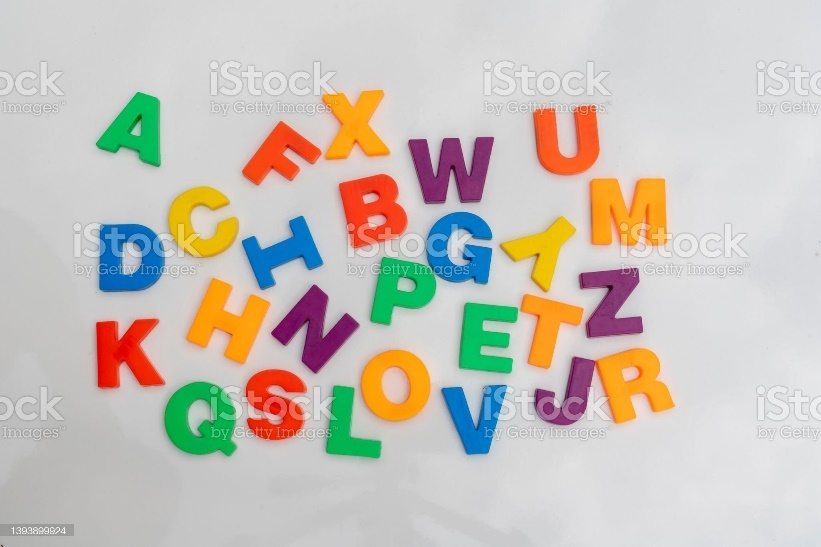
\includegraphics[width=3.72379in,height=2.48194in]{media/image1.jpeg}

Na língua portuguesa, há palavras que terminam com \textbf{-eza} e
palavras que terminam com \textbf{-esa}. Esses sufixos (terminações) são
pronunciados do mesmo modo, mas há regras próprias que devem ser
seguidas em seu uso. Observe os quadros a seguir.

\begin{longtable}[]{@{}l@{}}
\toprule
\begin{minipage}[t]{0.97\columnwidth}\raggedright\strut
O sufixo \textbf{-eza} transforma adjetivos em substantivos abstratos.

Exemplos: fraco -- fraqueza; delicado -- delicadeza; firme --
firmeza).\strut
\end{minipage}\tabularnewline
\bottomrule
\end{longtable}

\begin{longtable}[]{@{}l@{}}
\toprule
O sufixo \textbf{-esa} é usado para formar adjetivos pátrios no
feminino: (holandês -- holandesa; francês -- francesa; inglês --
inglesa; chinês -- chinesa; príncipe -- princesa; duque -- duquesa;
camponês -- camponesa; burguês -- burguesa).\tabularnewline
\bottomrule
\end{longtable}

As palavras terminadas em \textbf{-esa} fazem parte da classe gramatical
dos \textbf{adjetivos} e as palavras terminadas em \textbf{-eza} fazem
parte da classe gramatical dos \textbf{substantivos}.
}

\colorsec{Atividades}

Leia, agora, o início do conto \textbf{A roupa nova do imperador}. O
conto fala sobre um imperador muito vaidoso, que gostava de ter muitas
roupas, mas um dia ele foi enganado por dois falsos tecelões.

Oriente os alunos a realizar, primeiramente, leitura silenciosa do
texto, seguida de leitura em voz alta. Essa estratégia de leitura
possibilita que o aluno desenvolva fluência leitora, facilitando a
compreensão global do texto lido.

As atividades introdutórias são de compreensão do texto e têm a
finalidade de desenvolver habilidades de constatar, localizar
informações, realizar simples inferências, deduzir significados de
termos do texto e inferir o tempo em que ocorre a narrativa.

\textbf{A roupa nova do imperador}

%https://www.istockphoto.com/pt/vetorial/roman-emperor-vector-wearing-laurel-wreath-cartoon-character-gm1420622902-466533012?phrase=imperador\%20roupa

%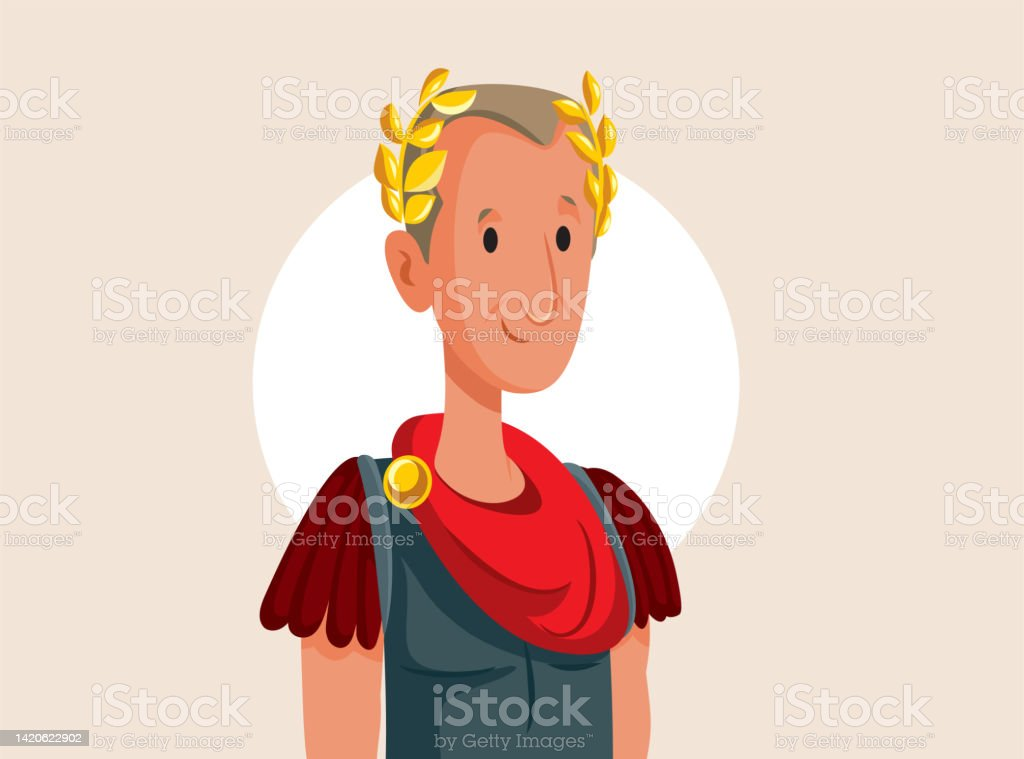
\includegraphics[width=4.23311in,height=3.13750in]{media/image2.jpeg}

\begin{quote}
Há muito, muito tempo, vivia em um reino distante um imperador
vaidosíssimo. Seu único interesse eram as roupas. Pensava apenas em
trocar de roupas, várias vezes ao dia; desfilava vestes belíssimas,
luxuosas e muito caras para a corte. Um belo dia, chegaram à capital do
reino dois pilantras, muito habilidosos em viver às custas do próximo.

Assim que os dois souberam da fraqueza do imperador por belas roupas,
espalharam a notícia de que eles eram especialistas em tecer um pano
único no mundo, de cores e padrões deslumbrantes. E --- o mais
impressionante, segundo eles: as roupas confeccionadas com aquele tecido
tinham o poder de serem invisíveis para as pessoas tolas, ou que
ocupassem um cargo sem merecê-lo. {[}...{]}
\end{quote}

\fonte{ANDERSEN, Hans Christian. \textbf{A roupa nova do imperador}. Disponível
em:
https://5ca0e999-de9a-47e0-9b77-7e3eeab0592c.usrfiles.com/ugd/5ca0e9\_5a4e21948da644a0bda95a1155c64c63.pdf.
Acesso em: 01 mar. 2023.}

\begin{tabular}{ll}
\textbf{Glossário} & \mbox{}\\
Pilantra & pessoa desonesta.\\
\end{tabular}

\num{1} Onde o imperador vivia?

\reduline{Em um reino distante.\hfill}
\linhas{2}

\num{2} Qual era o único interesse do imperador?

\reduline{Seu único interesse eram as roupas.\hfill}
\linhas{2}

\num{3} Qual foi a notícia que os dois pilantras espalharam ao saber da fraqueza
do imperador?

\reduline{Eles espalharam a notícia de que eles eram especialistas
em tecer um pano único no mundo, de cores e padrões deslumbrantes. E que
as roupas confeccionadas com aquele tecido tinham o poder de serem
invisíveis para as pessoas tolas, ou que ocupassem um cargo sem
merecê-lo.\hfill}
\linhas{4}

\num{4} Releia um trecho do conto e observe os termos destacados.

\begin{quote}
Assim que os dois souberam da \textbf{fraqueza} do imperador por
\textbf{belas} roupas, espalharam a notícia de que eles eram
especialistas em tecer um pano único no mundo, de cores e padrões
deslumbrantes.
\end{quote}

\begin{escolha}
\item
A que classe de palavras pertence o termo \textbf{belas}?

\reduline{À classe dos adjetivos.\hfill}

\item
A que classe de palavras pertence a palavra \textbf{fraqueza}?

\reduline{À classe dos substantivos.\hfill}
\end{escolha}

\num{5} Complete as frases com os \textbf{adjetivos} do quadro.

\begin{mdframed}[linewidth=2pt,linecolor=salmao,roundcorner=20pt]
\hfill\textbf{macia}\hfill \textbf{fraco}\hfill \textbf{gentil}\hfill
\end{mdframed}

\begin{escolha}
\item O resfriado que peguei me deixou muito \reduline{fraco\hfill}.

\item Ela é uma pessoa muito \reduline{gentil\hfill}.

\item A toalha do hotel era muito \reduline{macia\hfill}.
\end{escolha}

\num{6} Transforme os adjetivos que você usou para completar as frases da atividade
anterior em \textbf{substantivos}.

\reduline{Fraqueza\hfill}

\reduline{gentileza\hfill}

\reduline{maciez.\hfill}

\num{7} O escritor do conto que você leu, Hans Christian Andersen, nasceu na Dinamarca.

\begin{escolha}
\item Um rapaz que nasce na Dinamarca é \reduline{dinamarquês\hfill}.

\item Uma moça que nasce na Dinamarca é \reduline{dinamarquesa\hfill}.
\end{escolha}

\num{8} Observe as bandeiras a seguir e leia o nome dos respectivos países a que elas correspondem.

%\begin{itemize}
%\item
  %https://pixabay.com/pt/vectors/portugal-bandeira-bandeira-nacional-162394/
%\item
  %https://pixabay.com/pt/illustrations/bandeira-holanda-europa-2292675/
%\item
 % https://www.istockphoto.com/br/foto/bandeira-do-jap\%C3\%A3o-em-o-vento-gm492042302-75969761?utm\_source=pixabay\&utm\_medium=affiliate\&utm\_campaign=SRP\_image\_sponsored\&utm\_content=https\%3A\%2F\%2Fpixabay.com\%2Fpt\%2Fimages\%2Fsearch\%2Fbandeira\%2520jap\%25C3\%25A3o\%2F\&utm\_term=bandeira+jap\%C3\%%A3o
%\end{itemize}
%
%
\includegraphics[width=2.00012in,height=1.33333in]{media/image3.png}
%
\includegraphics[width=1.98958in,height=1.32631in]{media/image4.png}
%
\includegraphics[width=1.79857in,height=1.19792in]{media/image5.jpeg}

%Portugal Holanda Japão

Escreva na tabela o nome do país de origem e as nacionalidades correspondentes. Siga o exemplo.

\begin{longtable}[]{@{}lll@{}}
\toprule
\begin{minipage}[b]{0.32\columnwidth}\raggedright\strut
\textbf{País de origem}\strut
\end{minipage} & \begin{minipage}[b]{0.32\columnwidth}\raggedright\strut
\begin{quote}
\textbf{Nacionalidade masculina}
\end{quote}\strut
\end{minipage} & \begin{minipage}[b]{0.32\columnwidth}\raggedright\strut
\begin{quote}
\textbf{Nacionalidade feminina }
\end{quote}\strut
\end{minipage}\tabularnewline
\midrule
\endhead
\begin{minipage}[t]{0.32\columnwidth}\raggedright\strut
França\strut
\end{minipage} & \begin{minipage}[t]{0.32\columnwidth}\raggedright\strut
\begin{quote}
francês
\end{quote}\strut
\end{minipage} & \begin{minipage}[t]{0.32\columnwidth}\raggedright\strut
\begin{quote}
francesa
\end{quote}\strut
\end{minipage}\tabularnewline
Portugal & português & portuguesa\tabularnewline
Holanda & holandês & holandesa\tabularnewline
Japão & japonês & japonesa\tabularnewline
\bottomrule
\end{longtable}

\num{9} Em relação à terminação das palavras que você escreveu, o que é possível
concluir sobre a grafia delas?

\reduline{As palavras terminadas em \textbf{-ês} se
transformaram no feminino \textbf{-esa}.\hfill}
\linhas{3}

\num{10} No caça-palavras, encontre palavras femininas de nacionalidades dos
países de origem que estão no quadro. Em seguida, escreva as palavras
encontradas na linhas.

\begin{mdframed}[linewidth=2pt,linecolor=salmao,roundcorner=20pt]
\textbf{Holanda}\hfill \textbf{Albânia}\hfill \textbf{Escócia}\hfill \textbf{Finlândia}\hfill \textbf{Inglaterra}
\end{mdframed}

\begin{longtable}[]{@{}llllllllllll@{}}
\toprule
T & N & L & H & E & A & C & L & V & N & E & S\tabularnewline
\midrule
\endhead
I & W & G & O & A & M & E & I & E & A & D & N\tabularnewline
H & O & L & A & N & D & E & S & A & L & O & V\tabularnewline
I & E & I & F & N & T & R & D & O & T & E & P\tabularnewline
T & F & I & N & L & A & N & D & E & S & A & E\tabularnewline
I & O & N & I & T & S & U & T & C & L & V & I\tabularnewline
E & R & G & E & I & T & L & O & B & E & T & T\tabularnewline
E & O & L & W & N & S & C & A & H & E & A & P\tabularnewline
K & D & E & L & E & E & N & H & E & W & A & N\tabularnewline
I & R & S & S & S & E & T & L & E & R & H & U\tabularnewline
I & E & A & A & S & P & I & I & H & N & H & A\tabularnewline
O & S & I & A & L & U & D & T & S & A & T & I\tabularnewline
\bottomrule
\end{longtable}

\linhas{5}

\colorsec{Treino}

\num{1} Observe a bandeira da Inglaterra. %(Fácil)

%https://br.freepik.com/vetores-gratis/ilustracao-de-bandeira-reino-unido\_2807791.htm\#query=bandeira\%20inglaterra\&position=0\&from\_view=search\&track=ais

%
\includegraphics[width=5.90556in,height=3.11319in]{media/image6.jpeg}

Uma mulher e um homem que nascem na Inglaterra são, respectivamente.

\begin{escolha}
\item ingleza e inglezo.

\item inglaterra e inglaterro.

\item inglaterrana e inglaterrano.

\item inglesa e inglês.
\end{escolha}

\coment{Saeb: D7 - Relacionar, na
compreensão do texto, informações textuais com conhecimentos de senso
comum.

BNCC: EF04LP08: Reconhecer e grafar, corretamente, palavras derivadas
com os sufixos -agem, -oso, -eza, -izar/-isar (regulares morfológicas).}

(A) Incorreta. A formação do feminino e do masculino dos adjetivos
pátrios têm terminação -esa e ês.

(B) Incorreta. Essas palavras não correspondem às nacionalidades.

(C) Incorreta. Essas palavras não correspondem às nacionalidades.

(D) Correta. Inglesa e inglês são os adjetivos pátrios corretos.

\num{2} Analise um trecho de um dos contos populares tradicionais africanos, ``Oxóssi''.
%(Médio) 

\textbf{Oxóssi}

\begin{quote}
Olofin era um rei africano da terra de Ifé, lugar de origem de todos os
iorubás.

Cada ano, na época da colheita, Olofin comemorava, em seu reino, a Festa
dos Inhames.

Ninguém no país podia comer dos novos inhames antes da festa. Chegando o
dia, o rei se

instalava no pátio do seu palácio. Suas mulheres sentavam à sua direita,
seus ministros atrás dele, agitando leques e espanta-moscas, e os
tambores soavam para saudá-lo.

As pessoas reunidas comiam inhame pilado e bebiam vinho de palma. Elas
comemoravam e brincavam.
\end{quote}

\fonte{OXÓSSI. Disponível em:
www.dominiopublico.gov.br/download/texto/me000589.pdf.
Acesso em: 02 mar. 2023.}

No trecho de ``Oxóssi'', os tambores soavam com o objetivo de

\begin{escolha}
\item comemorar a colheita dos inhames.

\item permitir o início do jantar.

\item fazer homenagem ao rei durante a festa.

\item acompanhar os ministros na festa.
\end{escolha}

\coment{Saeb: D5 - Inferir o sentido de uma palavra ou expressão a partir do
contexto imediato.

BNCC: EF15LP03: Localizar informações explícitas em textos.}

(A) Incorreta. A função dos tambores era saudar o rei durante a
celebração.

(B) Incorreta. O início do jantar era no início da festa.

(C) Correta. Os tambores são tocados com a intenção de homenagear e
saudar o rei Olofin durante a Festa dos Inhames.

(D) Incorreta. Os ministros da festa acompanhavam o cortejo ao rei junto
aos tambores.

\num{3} Leia o texto a seguir. %(Difícil)

\textbf{Pequenas agricultoras}

\begin{quote}
As formigas cortadeiras cultivam seu próprio jardim dentro do
formigueiro.

{[}...{]}

Formigas cortadeiras, como as saúvas, são especializadas em cultivar
fungos.

Os pedacinhos de folhas que elas cortam são levados para câmaras
especiais dentro dos formigueiros onde servirão como base para crescimento desses
fungos. Essas câmaras são chamadas pelos cientistas de ``jardins de
fungos''.

Mas cortar e carregar todas aquelas folhinhas é só o início de um
trabalho minucioso de cultivo.

\fonte{PEDRO, Vinícius São. \textbf{Pequenas agricultoras}. Disponível em:
http://chc.org.br/artigo/pequenas-agricultoras/. Acesso em: 02 mar.
2023.}
\end{quote}

O texto ``Pequenas agricultoras'' tem a finalidade de informar sobre

\begin{escolha}
\item a importância dos fungos cultivados pelas formigas.

\item o trabalho das formigas cortadeiras.

\item o modo de cultivar um jardim.

\item o trabalho de agricultores.
\end{escolha}

\coment{Saeb: D1 - Localizar informações num texto.

BNCC: EF35LP03: Identificar a ideia central do texto, demonstrando
compreensão global.}

(A) Incorreta. O objetivo do texto é discorrer sobre o trabalho das
formigas cortadeiras.

(B) Correta. A finalidade do texto é informar os leitores sobre o
trabalho das formigas cortadeiras.

(C) Incorreta. O texto não expõe modos de cultivar um jardim.

(D) Incorreta. O texto não trata do trabalho dos agricultores, mas das
formigas cortadeiras.

\chapter{Cartas}
\markboth{Módulo 2}{}

\coment{Neste módulo, os alunos farão leitura de
cartas, considerando-se o aperfeiçoamento da compreensão de textos desse
gênero do campo da vida cotidiana. As atividades terão foco na
identificação do objetivo da produção -- no que se refere à incitação de
seus autores e eventuais argumentos para justificá-la -- e de elementos
da organização textual, assim como a exploração da linguagem empregada.\\
Habilidades BNCC: EF04LP10 EF04LP14 EF04LP27 EF35LP24 EF35LP26}

\colorsec{Habilidades SAEB}

\begin{itemize}
\item Reconhecer diferentes gêneros textuais.

\item Identificar elementos constitutivos de textos narrativos.

\item Identificar as marcas de organização de textos dramáticos.

\item Analisar os efeitos de sentido de verbos de enunciação.
\end{itemize}

%https://pixabay.com/pt/illustrations/envelope-carta-papel-magia-7076001/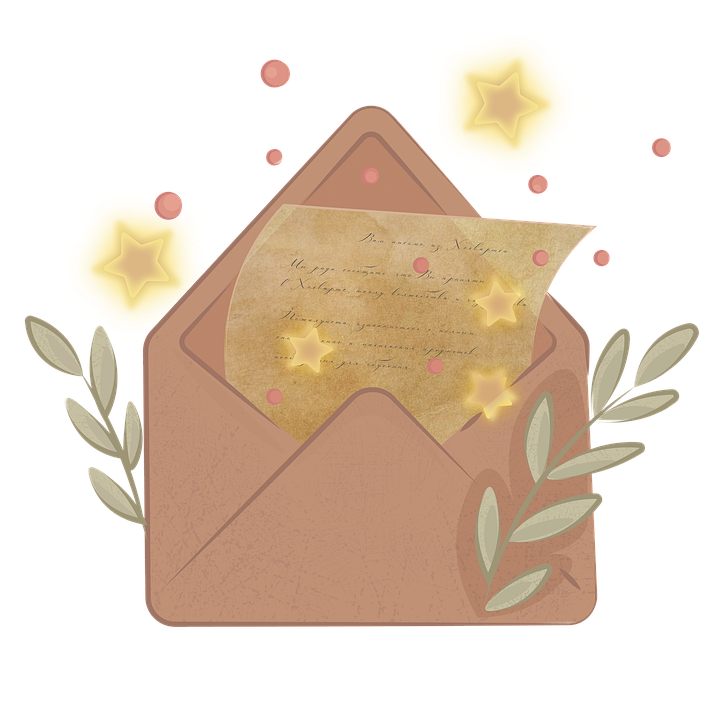
\includegraphics[width=3.59956in,height=3.60972in]{media/image7.png}

\conteudo{
\textbf{Cartas}

Quando o celular e a internet ainda não eram tão populares, um dos meios
mais utilizados para diminuir distâncias era a carta.

Sempre houve pessoas que gostavam de escrever cartas. E, ainda hoje,
mesmo com tantas outras possibilidades, existem pessoas que fazem
questão de escrever cartas aos amigos, parentes, etc.

A carta pessoal é uma mensagem que pode ser escrita à mão ou digitada. É
um texto escrito para alguém, ou seja, um destinatário, com o objetivo
de estabelecer contato com ele. A linguagem normalmente ocorre de modo
mais informal.

O envelope deve apresentar as informações de quem a envia no verso
(remetente) e de quem deverá receber a carta na frente (destinatário).
As informações de destinatário servem para que o serviço de Correios
localize onde a carta deve chegar. Para isso, ambas as informações devem
conter nome, endereço completo (rua, número, bairro, cidade e estado) e
CEP (código de endereçamento postal).

O conteúdo da carta deve vir em uma folha dentro do envelope, e deverá
ser aberta apenas pelo destinatário a quem a carta foi endereçada.

Hoje em dia, entretanto, há outros meios de manter esse diálogo, como o
celular e os aplicativos de mensagens instantâneas e os \emph{e-mails}.

Existem três tipos básicos de carta, independente da maneira como será
transmitida: a correspondência oficial e a correspondência comercial e a
correspondência pessoal.
}

\colorsec{Atividades}

Leia a carta pessoal a seguir.

\coment{Realize uma leitura compartilhada do texto. Chame a atenção dos alunos
para as rubricas no texto e para sua função de orientar a dramatização
(como indicações das formas de falar, caminhar, gesticular; indicação de
características como altura da voz, ritmo. Solicite aos alunos que
observem quem são as personagens e o papel de cada um.}

%Inserir imagem texto na carta em branco: \url{https://www.pexels.com/pt-br/foto/em-branco-vazio-cartao-ficha-7958171/}

\begin{quote}
\begin{flushright}
Fortaleza, 03 de março de 2023.
\end{flushright}

Olá, amado papai!

Estou bem com os padrinhos aqui em Fortaleza, mas tenho muita saudade de
você e de todos da família. Quando eu terminar o curso que vim fazer
aqui, volto para casa. Gostei muito dos lugares que conheci em
Fortaleza, como as praias e os parques aquáticos, mas sinto falta de
vocês e dos meus amigos de infância. Escrevo só para dizer isso, que
estou bem e o quanto sinto falta de tudo e de todos daí.

\begin{flushright}
Beijos para todos,

Gui
\end{flushright}
\end{quote}

%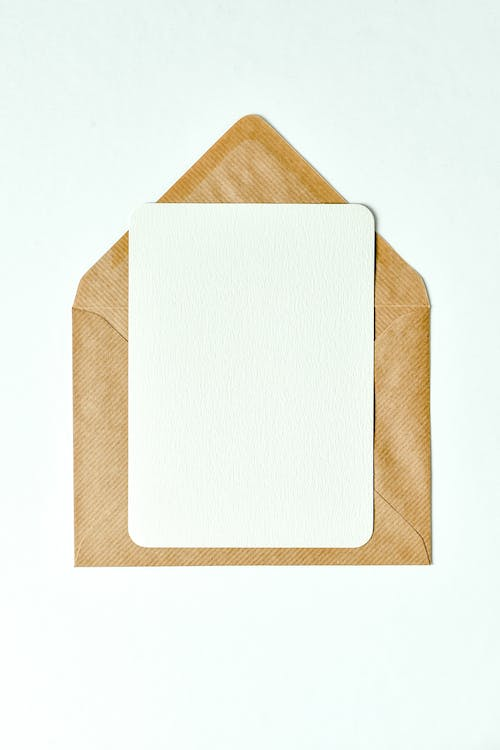
\includegraphics[width=3.60417in,height=5.40625in]{media/image8.jpeg}

\num{1} O que são cartas pessoais?

\reduline{São correspondências trocadas entre pessoas.\hfill}
\linhas{2}

\num{2} Quem escreveu a carta?

\reduline{Guilherme\hfill}
\linhas{1}

\num{3} Quem recebeu a carta?

\reduline{O pai do Guilherme\hfill}
\linhas{1}

\num{4} De onde Guilherme escreveu a carta?

\reduline{De Fortaleza\hfill}
\linhas{1}

\num{5} Como é composta a saudação da carta lida e o que ela indica sobre a
relação entre remetente e destinatário?

\reduline{``Olá, amado papai!'' é a saudação que indica que o remetente é filho do
destinatário, no caso, Guilherme, e a trata com afetividade, com a
adoção de ``querido'' e de ``papai'', no lugar de ``pai''.\hfill}
\linhas{2}

\num{6} Qual é o assunto da carta?

\reduline{Na carta a seu pai, Guilherme conta que está
bem, o que mais gostou em Fortaleza, quando pretende voltar para casa, e
a saudade que está sentindo dos familiares e amigos de infância.\hfill}
\linhas{2}

\num{7} A carta pessoal apresentada tem uma linguagem formal ou informal?
Justifique sua resposta.

\reduline{A carta pessoal normalmente é escrita de modo informal, tendo em vista
que é caracterizada por ser uma correspondência entre pessoas íntimas,
com demonstração de afetividade e carinho e a formalidade tornaria a
escrita mais distanciada e neutra.\hfill}
\linhas{2}

\num{8} O texto apresentado é teatral. Com qual objetivo esses textos são
escritos?

\reduline{O objetivo de se escrever textos desse tipo é para que sejam encenados.\hfill}
\linhas{2}

\num{9} Leia a carta a seguir e responda às questões propostas.

Criar uma carta com bordas.

\begin{mdframed}[linewidth=10pt,linecolor=salmao!20,backgroundcolor=salmao!20,roundcorner=20pt]
Curitiba, 12 de fevereiro de 2023.

\emph{Querida filha Cecília},

Estou morrendo de saudades...

Por aqui, a vida está exatamente igual, seus irmãos e seu pai também
estão bem, e sentem muitas saudades de você.

Filhinha, você está fazendo o certo. Ir a São Paulo estudar vai te
ajudar muito a conseguir o emprego dos seus sonhos.

Aproveite muito filha, ajude a sua prima Sofia com as tarefas domésticas
e agradeça sempre por ela ter recebido você na casa dela.

\begin{flushright}
Beijo,

Mamãe.
\end{flushright}
\end{mdframed}

\begin{escolha}
\item \textbf{Vocativo} é o modo como é denominado quando chamamos uma
pessoa com quem estamos nos comunicando. Sublinhe o vocativo da carta
acima.

\item Quem escreveu a carta?

\begin{boxlist}
\boxitem[\rosa{X}] a mãe de Cecília 

\boxitem[] Sofia

\boxitem[] Cecília
\end{boxlist}

\item Quem é Cecília com relação a pessoa que escreve a carta??

\reduline{Filha.\hfill}

\item Quem é o destinatário dessa carta?

\reduline{Cecília.\hfill}


e) Escreva qual foi a despedida da carta. 

\reduline{Beijo, Mamãe.\hfill}

\colorsec{Treino}

\num{1} Leia a carta pessoal a seguir para responder à questão.

%(Fácil) 

\begin{mdframed}[linewidth=10pt,linecolor=salmao!20,backgroundcolor=salmao!20,roundcorner=20pt]
São Paulo, 01 de março de 2023.

Querida vó,

Como a senhora está? Estou com muitas saudades de você e mal posso
esperar pelo Natal, quando vamos nos reunir e relembrar os tempos de
infância. Estar longe de você tem sido muito triste, mas guardo os seus
conselhos que me ajudam a superar as dificuldades.

\begin{flushright}
Até breve!

Sandra
\end{flushright}
\end{mdframed}

O elemento ``Até breve,'' da carta lida, representa a:

\begin{escolha}
\item assinatura.

\item despedida.

\item saudação.

\item reclamação.
\end{escolha}

\coment{Saeb: D5 - Inferir o sentido de uma palavra ou expressão a partir do
contexto imediato.

BNCC: EF04LP10: Ler e compreender, com autonomia, cartas pessoais de
reclamação, dentre outros gêneros do campo da vida cotidiana, de acordo
com as convenções do gênero carta e considerando a situação comunicativa
e o tema/assunto/finalidade do texto.}

(A) Incorreta. A assinatura é seguida da despedida.

(B) Correta. O elemento transcrito ``Até breve'' é a despedida da carta
lida.

(C) Incorreta. A saudação abre, e não encerra a carta.

(D) Incorreta. Não há reclamação na carta lida.

\num{2} Releia a carta pessoal a seguir para responder à questão.

%(Médio) 

\begin{mdframed}[linewidth=10pt,linecolor=salmao!20,backgroundcolor=salmao!20,roundcorner=20pt]
São Paulo, 01 de março de 2023.

Querida vovó,

Como a senhora está? Estou com muitas saudades de você e mal posso
esperar pelo Natal, quando vamos nos reunir e relembrar os tempos de
infância. Estar longe de você tem sido muito triste, mas guardo os seus
conselhos que me ajudam a superar as dificuldades.

\begin{flushright}
Até breve!

Sandra
\end{flushright}
\end{mdframed}

Que saudação também seria adequada ao contexto dessa carta?

\begin{escolha}
\item Prezada vovó.

\item Olá, vovó!

\item Avó.

\item Atenciosamente.
\end{escolha}

\coment{Saeb: D5 - Inferir o sentido de uma palavra ou expressão a partir do
contexto imediato.

BNCC: BNCC: EF04LP10: Ler e compreender, com autonomia, cartas pessoais
de reclamação, dentre outros gêneros do campo da vida cotidiana, de
acordo com as convenções do gênero carta e considerando a situação
comunicativa e o tema/assunto/finalidade do texto.}

(A) Incorreta. A saudação é mais formal e não se adequaria ao contexto
de correspondência entre avó e neta.

(B) Correta. ``Olá, vovó!'' seria equivalente a ``Querida vovó'',

(C) Incorreta. Somente o nome do destinatário no vocativo não revelaria
intimidade, como ocorre na saudação original

(D) Incorreta. ``Atenciosamente'' é mais adequado à despedida de uma
carta, além de não ser íntima e pessoal, como o contexto da carta.

\num{3} Leia a carta de uma leitora para a revista de publicações
científicas denominada \textit{Planeta}.

%(Difícil) 

\textbf{Evolução com consciência}

\begin{quote}
Sou leitora e apreciadora assídua de PLANETA. Quero parabenizar Ricardo
Arnt por estar assumindo a direção de redação. Aproveito para desejar a
toda a equipe da revista um tempo de muita paz e luz. Tenho acompanhado
muitas mudanças, algumas muito positivas e outras, a meu ver, não tão
positivas sobre a filosofia da revista, mas mudanças não podem agradar a
todos. O importante é que continue a ser uma publicação que nos ajude em
nosso evoluir com consciência, mesmo que por trilhas diferenciadas das
antigas.

\begin{flushright}
Almira Lima, Rio Grande, RS, por \emph{e-mail}.
\end{flushright}
\end{quote}

\fonte{LIMA, Almira. \textbf{Evolução com consciência}. Revista Planeta.
Disponível em: www.revistaplaneta.com.br/cartas-15/. Acesso em: 03 mar. 2023.}

\begin{tabular}{ll}
\textbf{Glossário} & \mbox{}\\
assídua & com bastante frequência.\\
\end{tabular}

Uma das informações presentes nessa carta é

\begin{escolha}
\item o remetente, visto em ``Planeta''.

\item a despedida, vista em ``desejar muita paz e luz''.

\item o título, visto em ``sou leitora e apreciadora''.

\item a localização da leitora, vista em ``Rio Grande''.
\end{escolha}

\coment{Saeb: D1 - Localizar informações num texto.

BNCC: EF04LP10: Ler e compreender, com autonomia, cartas pessoais de
reclamação, dentre outros gêneros do campo da vida cotidiana, de acordo
com as convenções do gênero carta e considerando a situação comunicativa
e o tema/assunto/finalidade do texto.}

(A) Incorreta. O remetente é quem escreve a carta.

(B) Incorreta. Essa carta não apresenta uma despedida.

(C) Incorreta. O título é ``Evolução com consciência''.

(D) Correta. A leitora da carta resolveu colocar, em sua identificação,
o local no qual ela está e escreve para a revista.

\chapter{Textos instrucionais}
\markboth{Módulo 3}{}

\coment{Neste módulo, espera-se que os alunos
reconheçam as características de textos instrucionais em manuais, assim
como as características de textos instrucionais, passo a passo, verbos
no imperativo e demais recursos de linguagem relativos ao gênero textual.\\
Habilidades BNCC: EF04LP13.}

\colorsec{Habilidades SAEB}

\begin{itemize}
\item Analisar elementos constitutivos de gêneros textuais diversos.

\item Reconhecer os usos da pontuação.

\item Analisar os efeitos de sentido decorrentes do uso da pontuação.
\end{itemize}

\conteudo{
\textbf{Textos instrucionais}

%\textbf{https://br.freepik.com/vetores-gratis/manual-de-instrucoes-guia-documento-com-elemento-de-design-isolado-de-roda-dentada-arquivo-de-analise-de-personagem-masculino-analise-de-negocios-processamento-de-dados-atualizacao\_12083052.htm\#page=4\&query=manual\&position=3\&from\_view=search\&track=sph}

%
\includegraphics[width=2.93750in,height=2.93750in]{media/image9.jpeg}

No nosso dia a dia, em diversas situações, precisamos ler textos que nos
ajudem a executar uma tarefa. Quando queremos fazer um biscoito, por
exemplo, procuramos uma receita, lemos um manual quando queremos saber
quais são as regras de um jogo ou a bula quando queremos compreender o
modo de tomar determinada medicação. Todos esses textos que nos
direcionam a ações que devemos tomar para atingir certa finalidade são
denominados instrucionais, tendo em vista que nos fornecem instruções.
Os textos instrucionais têm por objetivo nos informar como devemos
proceder para realizar a tarefa que queremos realizar, para isso, são
objetivos, diretos e esclarecedores. Eles também utilizam verbos, como
``precisar'', ``necessitar'' e ``dever'' para informar ao leitor os
procedimentos para atingir certa finalidade.
}

\colorsec{Atividades}

\num{1} Leia o texto a seguir. Em seguida, responda às atividades propostas.

%\url{https://www.istockphoto.com/br/foto/sumo-de-beterraba-gm1178095232-329133307?utm_source=pixabay\&utm_medium=affiliate\&utm_campaign=SRP_image_sponsored\&utm_content=https\%3A\%2F\%2Fpixabay.com\%2Fpt\%2Fimages\%2Fsearch\%2Fsuco\%2520beterraba\%2F\&utm_term=suco+beterraba}

%https://www.gov.br/saude/pt-br/assuntos/saude-brasil/eu-quero-me-alimentar-melhor/noticias/2018/suco-rico-em-fibras-5-receitas-para-misturar-frutas-e-vegetais/

%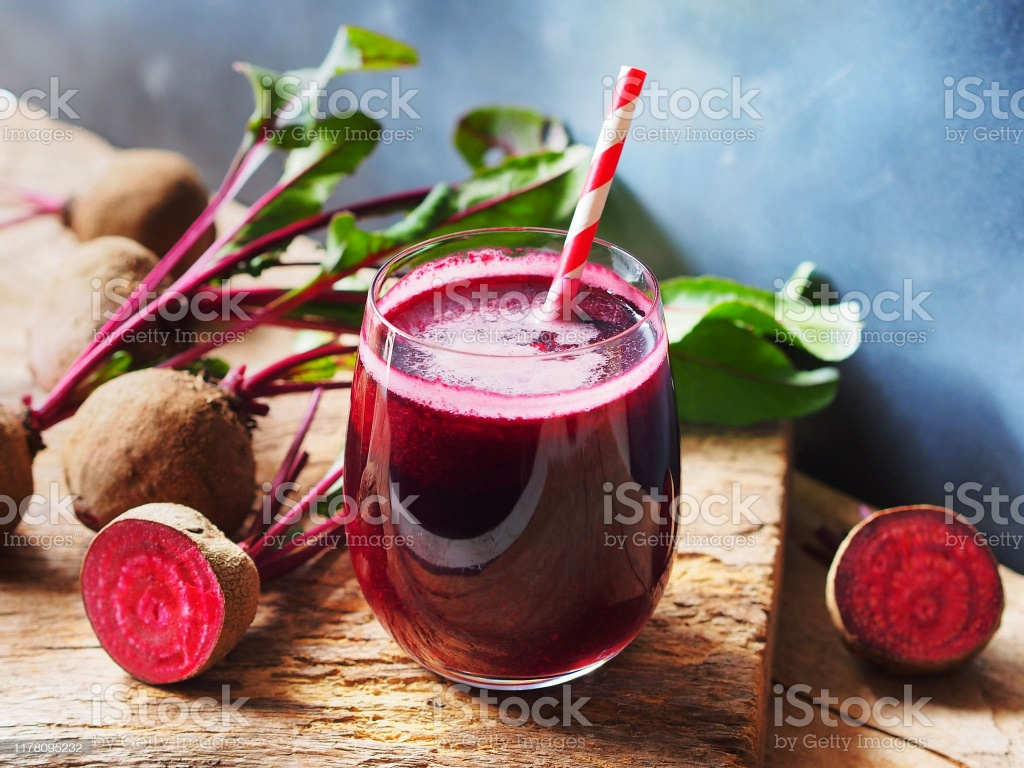
\includegraphics[width=4.65278in,height=3.48958in]{media/image10.jpeg}

\textbf{Suco de beterraba com limão}

\textbf{INGREDIENTES}

2 copos americanos duplos de água\\
1 beterraba média\\
1 limão sem casca e sementes\\
1 colher de sopa de açúcar

\textbf{MODO DE PREPARO}

Misture tudo no liquidificador. Se desejar, coloque gelo e sirva.

\textbf{RENDIMENTO}

3 porções.

DICA: O limão pode ser substituído por laranja ou maracujá.

\fonte{Disponível em:
https://www.gov.br/saude/pt-br/assuntos/saude-brasil/eu-quero-me-alimentar-melhor/noticias/2018/suco-rico-em-fibras-5-receitas-para-misturar-frutas-e-vegetais/.
Acesso em: 5 mar. 2023.}

\item Por que podemos dizer que o texto lido é do tipo instrucional?

\reduline{O texto lido pode ser considerado instrucional porque é uma receita de
suco, ou seja, propõe-se a ensinar como prepará-los. Para isso, dá
instruções do que deve ser feito pelo leitor, quais são os ingredientes
necessários, modo de preparo e rendimento.\hfill}

\item Qual é a quantidade de beterraba e de açúcar que devem ser utilizadas
para realizar a receita?

\reduline{A quantidade de beterraba a ser utilizada na
receita é 1 beterraba média e a quantidade de açúcar é 1 colher.\hfill}

\item Como você descobriu essa informação?

\reduline{A informação está presente no trecho dos ingredientes da receita.\hfill}

\item No modo de preparo, por que não é necessário expor a quantidade de
ingredientes que devem ser utilizadas?

\reduline{Porque ela já foi informada na parte dos ingredientes\hfill}

\num{2} Releia este trecho da receita atentando aos verbos destacados:

\begin{quote}
\textbf{Misture} tudo no liquidificador. Se desejar, \textbf{coloque} gelo e sirva.
\end{quote}

\begin{escolha}
\item
  Os verbos destacados foram utilizados no texto para:

\begin{boxlist}
\boxitem[] mostrar quem faz a ação.

\boxitem[\rosa{X}] fazer pedidos.

\boxitem[] dar instruções.

\boxitem[] indicar o tempo em que a ação acontece.
\end{boxlist}

\item
  Os verbos destacados estão no modo:

\begin{boxlist}
\boxitem[\rosa{X}] imperativo

\boxitem[] afirmativo
\end{boxlist}

\end{escolha}

\num{3} Leia o passo a passo de como fazer um coração de origami.

%Arte: Pedir autorização do texto e imagem a seguir ou solicitar ilustração conforme modelo a seguir. 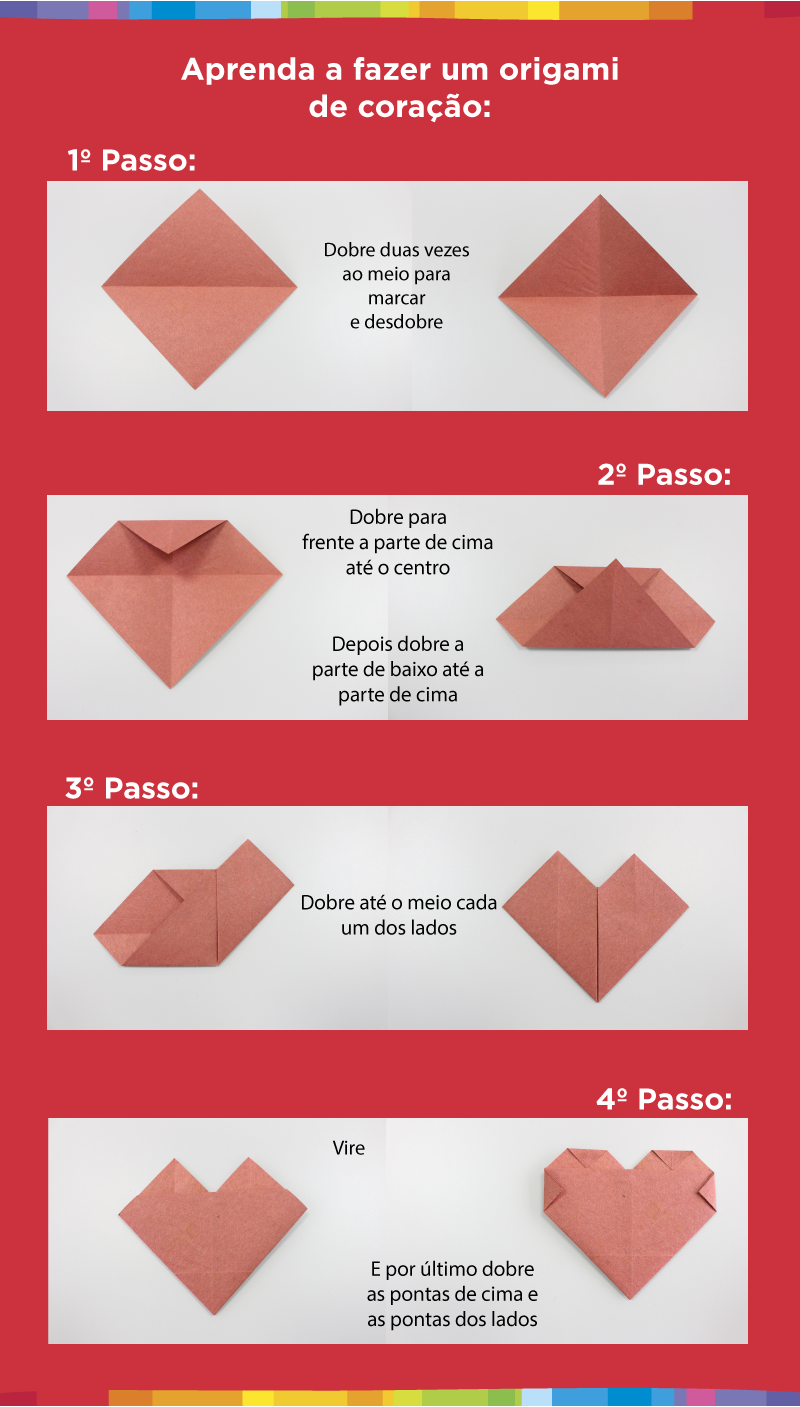
\includegraphics[width=4.87700in,height=8.57778in]{media/image11.png}

%Disponível em: https://blog.brandili.com.br/diy-como-fazer-um-origami-de-coracao/. Acesso em: 6 mar. 2023.

\begin{escolha}
\item Por que o texto lido pode ser considerado um texto instrucional? Justifique sua resposta.

\reduline{É considerado texto instrucional por conta de sua estrutura, com divisões e organização, auxiliando o leitor a realizar determinada tarefa, oferecendo instruções.\hfill}

\item Qual é o objetivo do texto lido?

\reduline{O objetivo do texto lido é ensinar a fazer um origami em forma de coração.\hfill}

\item Que características do texto instrucional podem ser encontradas no texto lido?

\reduline{O texto lido tem por característica de texto instrucional porque seu
objetivo é ensinar e instruir; apresentando na estrutura frasal verbos
como ``dobre, desdobre'', no imperativo; e o passo a passo de como fazer
as dobraduras.\hfill}

\colorsec{Treino}

\num{1} Leia o texto a seguir.

%(Fácil)
%https://pixabay.com/pt/illustrations/fruta-cesta-tigela-fresco-cerejas-5004282/
\includegraphics[width=3.05646in,height=2.55903in]{media/image12.jpeg}

\textbf{Salada de frutas}

\textbf{Ingredientes:}

\begin{itemize}
\item 1 maçã

\item 3 bananas

\item ½ mamão

\item 1 lata de leite condensado (opcional) ou açúcar.
\end{itemize}

\textbf{Modo de preparo:}

Lave bem todas as frutas. retire a casca e as sementes. corte as frutas
e quadradinhos. coloque o leite condensado ou o açúcar. misture e leve à
geladeira por 30 minutos.

O texto lido pode ser classificado como:

\begin{escolha}
\item
  receita culinária.
\item
  reportagem.
\item
  instrução de jogos.
\item
  fábula.
\end{escolha}

\coment{Saeb: D4 - Identificar o tema central do texto.

BNCC: EF04LP13: Identificar e reproduzir, em textos injuntivos
instrucionais (instruções de jogos digitais ou impressos), a formatação
própria desses textos (verbos imperativos, indicação de passos a ser
seguidos) e formato específico dos textos orais ou escritos desses
gêneros (lista/ apresentação de materiais e instruções/passos de jogo).}


(A) Correta. O texto lido pode ser classificado como receita culinária.

(B) Incorreta. O gênero reportagem é um texto informativo, e não
instrucional.

(C) Incorreta. O texto lido é instrucional, mas não pode ser
classificado como receita culinária.

(D) Incorreta. Fábulas são da esfera da narrativa.


\num{2} Leia o texto instrucional a seguir.

%(Médio)

\textbf{Quem toca mais, ganha}

\textbf{Material necessário}\\
1 bola

\textbf{Modo de jogar}\\
Em um campo aberto {[}\ldots{}{]} duas equipes {[}\ldots{}{]} têm como
objetivo trocar o maior número possível de passes {[}\ldots{}{]}.

Cada toque representa um número na contagem, que deve ser feita
paralelamente aos passes, em voz alta.

Quando um passe sofrer interferência da equipe adversária, a contagem
recomeça do zero.

\fonte{QUEM TOCA mais, ganha. In: ABREU, Ana Rosa (org.). Alfabetização: livro
do aluno. Brasília: FUNDESCOLA/SEF-MEC, 2000, vol. 3, p. 35. Disponível
em: www.dominiopublico.gov.br/download/texto/me000590.pdf. Acesso em: 6 mar.
2023.}

Em relação à estrutura do texto instrucional, pode-se identificar a
presença de

\begin{escolha}
\item títulos que mostram como se obter o material e os participantes.

\item subtítulos que explicam como funciona o material ``bola''.

\item subtítulos que marcam o material necessário e como jogar a brincadeira.

\item títulos que apresentam diferentes modos de se jogar o jogo.
\end{escolha}

\coment{Saeb: D9 - Realizar inferências e antecipações em relação ao conteúdo e
à intencionalidade a partir de indicadores como tipo de texto e
características gráficas.

BNCC: EF04LP13: Identificar e reproduzir, em textos injuntivos
instrucionais (instruções de jogos digitais ou impressos), a formatação
própria desses textos (verbos imperativos, indicação de passos a ser
seguidos) e formato específico dos textos orais ou escritos desses
gêneros (lista/ apresentação de materiais e instruções/passos de jogo).}

(A) Incorreta. O texto apresenta somente um título, o que marca o nome
da brincadeira.

(B) Incorreta. O texto não trata sobre o funcionamento da bola.

(C) Correta. Tendo por base os subtítulos ``Material necessário'' e
``Modo de jogar'' e de seus conteúdos, infere-se que a estrutura é de
texto instrucional.

(D) Incorreta. O texto tem apenas um título, o nome da brincadeira, e um
modo de se jogar a brincadeira.

\num{3} Leia o trecho de um manual.
%(Difícil) 

\begin{quote}
{[}...{]}

UNO® é recomendado para crianças e adultos a partir de 7 anos de idade e número de jogadores pode variar entre 2 e 10 pessoas.

\textbf{Baralho}\\
Para jogar UNO® é necessário comprar um baralho próprio para o jogo,
{[}...{]}.

Esse baralho é composto por 108 cartas {[}...{]}

\textbf{Objetivo}\\
Ser o primeiro jogador a fazer 500 pontos. Para fazer pontos, você deve
livrar-se o quanto antes de todas as cartas da sua mão e usar as cartas de ação
para evitar que os adversários façam o mesmo. A quantidade de pontos que você
ganha é a soma dos números das cartas dos oponentes.
\end{quote}

\fonte{UNO. Jogos de carta. Disponível em:
http://webcache.googleusercontent.com/search?q=cache:FfXgMOckOtYJ:jogosdecartas.hut.com.br/uno/\&cd=11\&hl=pt-BR\&ct=clnk\&gl=br.
Acesso em: 6 mar. 2023.}

Conforme informações do texto, para ganhar o jogo a pessoa deve

\begin{escolha}
\item ser a primeira a fazer 500 pontos.

\item possuir pelo menos uma carta nas mãos.

\item evitar usar as cartas de ação durante o jogo.

\item ter menos pontos que as cartas dos oponentes.
\end{escolha}

\coment{Saeb: D1 - Localizar informações num texto.

BNCC EF03LP16: Identificar e reproduzir, em textos injuntivos
instrucionais (receitas, instruções de montagem, digitais ou impressos),
a formatação própria desses textos (verbos imperativos, indicação de
passos a ser seguidos) e a diagramação específica dos textos desses
gêneros (lista de ingredientes ou materiais e instruções de execução --
"modo de fazer").}

(A) Correta. A finalidade do jogo é ser o primeiro jogador a fazer 500
pontos.

(B) Incorreta. O jogador deve se livrar de todas as cartas.

(C) Incorreta. O jogador precisa utilizar as cartas de ação para evitar
que os adversários se livrem de todas as suas cartas.

(D) Incorreta. O jogador precisa ter 500 pontos, o que será calculado
conforme a soma das cartas dos adversários.

\chapter{Módulo 4}
\markboth{Módulo 4}{}

\coment{Neste módulo, espera-se que os alunos leiam
e compreendam autonomamente texto do campo da vida pública; relacionem a
imagem no texto à mensagem (linguagens verbal e não verbal); relacionem
a finalidade do texto às estratégias de convencimento; identifiquem a
função social do texto, reconhecendo para que serve e a quem se destina;
identifiquem a ideia central do texto, compreendendo-o globalmente e
infiram informações implícitas no texto.\\
Habilidades BNCC: EF03LP19}

\colorsec{Habilidades SAEB}

\begin{itemize}
\item Analisar o uso de recursos de persuasão em textos verbais e/ou multimodais.

\item Analisar os efeitos de sentido de recursos multissemióticos em textos que circulam em diferentes suportes.

\item Julgar a eficácia de argumentos em textos.
\end{itemize}

\conteudo{
\textbf{Anúncio publicitário}

%\textbf{https://pixabay.com/pt/photos/cartazes-muro-propaganda-679177/}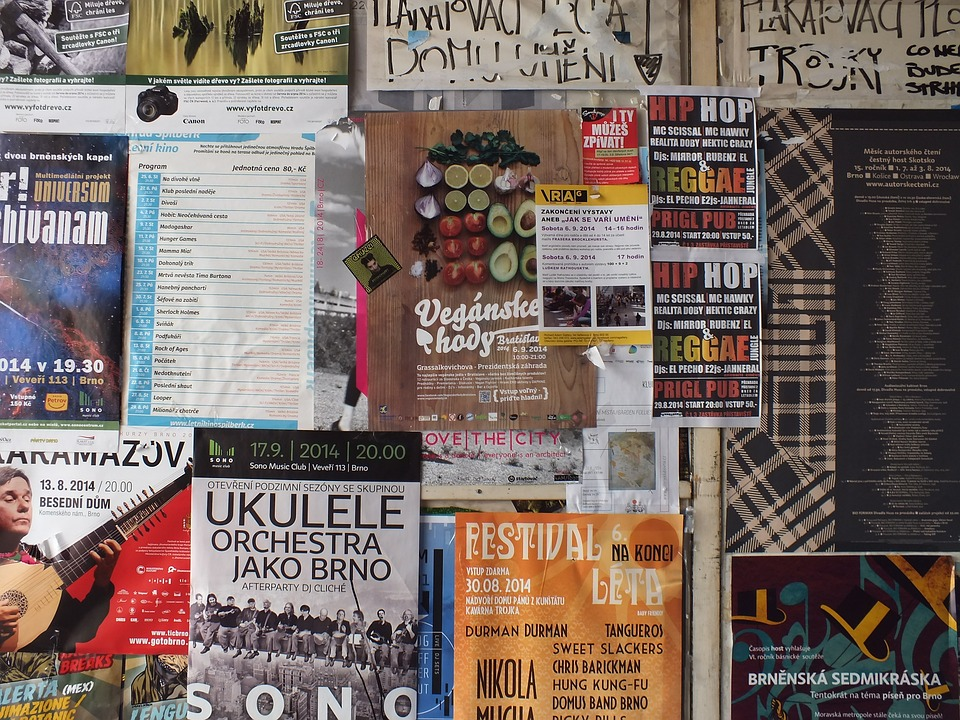
\includegraphics[width=5.90556in,height=4.42917in]{media/image13.jpeg}

Anúncio publicitário consiste em um tipo textual com a finalidade de
convencer o leitor a consumir um produto ou serviço. Para esse objetivo,
utiliza linguagem persuasiva, misturando recursos visuais, como cores,
formas, símbolos, figuras, imagens fictícias, entre outros, com uma
linguagem cheia de afeto, emoções com a intenção de envolver o
consumidor em um jogo linguístico, despertar o interesse e incentivar
vontades que o levem a comprar o produto ou o serviço.

Campanha publicitária consiste no conjunto de peças publicitárias,
criado por uma agência publicitária, a fim de divulgar um produto ou
determinada ideia.
}

\colorsec{Atividades}

\num{1} O dia 20 de novembro foi oficialmente incluído como uma data em
referência à consciência negra. Leia este cartaz publicitário.

Explore com os alunos o cartaz, a imagem que o compõe e os elementos
verbais. Avalie com eles os motivos da escolha do produtor ao dar ênfase
a alguns elementos do texto verbal, e se esse recurso foi efetivo na
divulgação do que ele pretendia.

%https://www.guiricema.mg.gov.br/20-de-novembro-dia-da-consciencia-negra/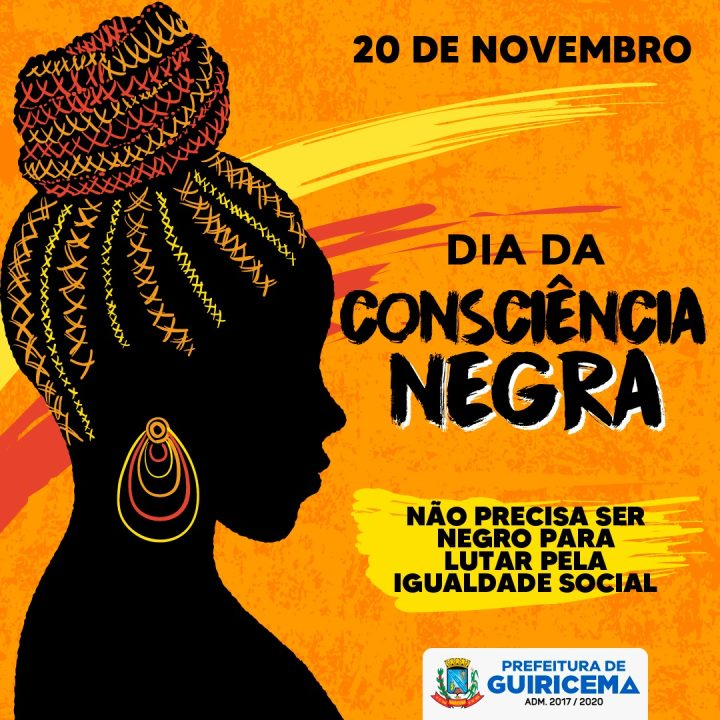
\includegraphics[width=5.28125in,height=5.28125in]{media/image14.jpeg}

\begin{escolha}
\item O cartaz da campanha do \textbf{Dia da Consciência Negra} foi feito para:

\begin{boxlist}
\boxitem[\rosa{X}] convencer as pessoas em relação à importância de lutar pela igualdade racial.

\boxitem[] convencer as pessoas em relação à importância de todos terem acesso à vacinação.

\boxitem[] sensibilizar as pessoas, como ocorre nas poesias.
\end{boxlist}

\item Releia o \emph{slogan} do cartaz.

\begin{mdframed}[linewidth=10pt,linecolor=salmao!20,backgroundcolor=salmao!20,roundcorner=20pt]
\textbf{Não precisa ser negro para lutar pela igualdade racial}
\end{mdframed}

Que sentido pode ter essa frase? Converse com os colegas e escreva a
conclusão a que chegaram nas linhas a seguir.

\reduline{Resposta pessoal.
Explique aos alunos que, embora no Brasil haja uma intensa mistura de
raças, a incidência de racismo pode não ser tão evidente para
determinadas pessoas, mas ele não deixa de existir. Em alguns casos,
ele ocorre de forma sutil, em que nem é percebido pelas pessoas. É
necessário fortalecer a identidade étnico-racial e respeitar as
diversidades.\hfill}

\item Quem promoveu esse cartaz?

\reduline{A Prefeitura de Guiricema.\hfill}

\item Em sua opinião, o anúncio está cumprindo seu propósito? Justifique sua resposta.

\reduline{Resposta pessoal.\hfill}
\end{escolha}

\num{2} Leia, a seguir, o cartaz de promoção do Festival Nacional do Teatro
Infantil, de Feira de Santana, Bahia.

%https://jornalgrandebahia.com.br/2017/09/a-festa-do-teatro-infantil-brasileiro-vai-comecar-em-feira-de-santana/ 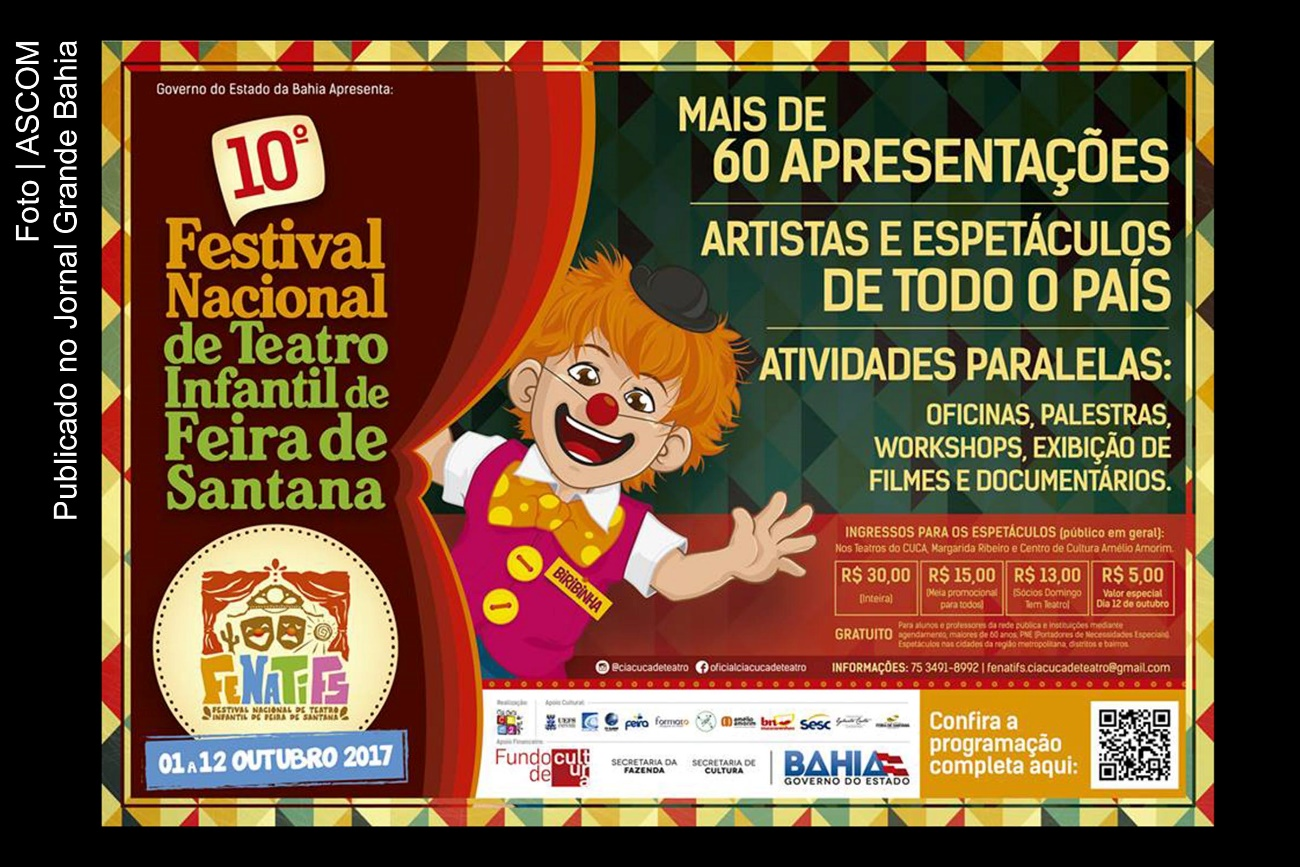
\includegraphics[width=5.90556in,height=3.93681in]{media/image15.jpeg}

\begin{escolha}
\item Quais estratégias, na composição dessa capa, contribuem para
incentivar as pessoas a participar do festival?

\reduline{Os alunos podem citar o
colorido do cartaz, a ilustração de uma criança com nariz de palhaço e
roupa de bilheteiro, a quantidade atrações no festival e as atividades
paralelas que serão realizadas durante o evento.\hfill}

\item Quantas vezes ocorreram o Festival Nacional de Teatro Infantil de
Feira de Santana?

\reduline{10 vezes\hfill}

\item Quais são as atividades paralelas que vão ocorrer durante o festival?

\reduline{Oficinas, palestras, \emph{Workshops}, exibição de filmes e documentários.\hfill}

\item As cores e letras usadas no cartaz foram utilizadas com o objetivo de:

\begin{boxlist}
\boxitem[] deixá-lo mais bonito.

\boxitem[\rosa{X}] destacar a mensagem escrita.

\boxitem[] destacar um produto
\end{boxlist}

\item Em sua opinião, por que foi usado um desenho de um personagem infantil no cartaz?

\reduline{Para atrair a atenção desse público-alvo.\hfill}

\item Quando esse festival aconteceu? 

\reduline{De 01 a 12 de outubro de 2017.\hfill}
\end{escolha}

\num{3} Você sabe o que é um \textbf{festival}? Junte-se a um colega e pesquisem
no dicionário o significado dessa palavra e registre-o a seguir.

\reduline{Sugestão de resposta: Diversos eventos ou espetáculos culturais, com
diversas apresentações, podendo ocorrer periodicamente.\hfill}
\linhas{5}

\num{4} Leia, agora, outro anúncio de campanha publicitária.

%https://www.facebook.com/daejundiai/photos/a.609606715910778/1544172665787507/?type=3
%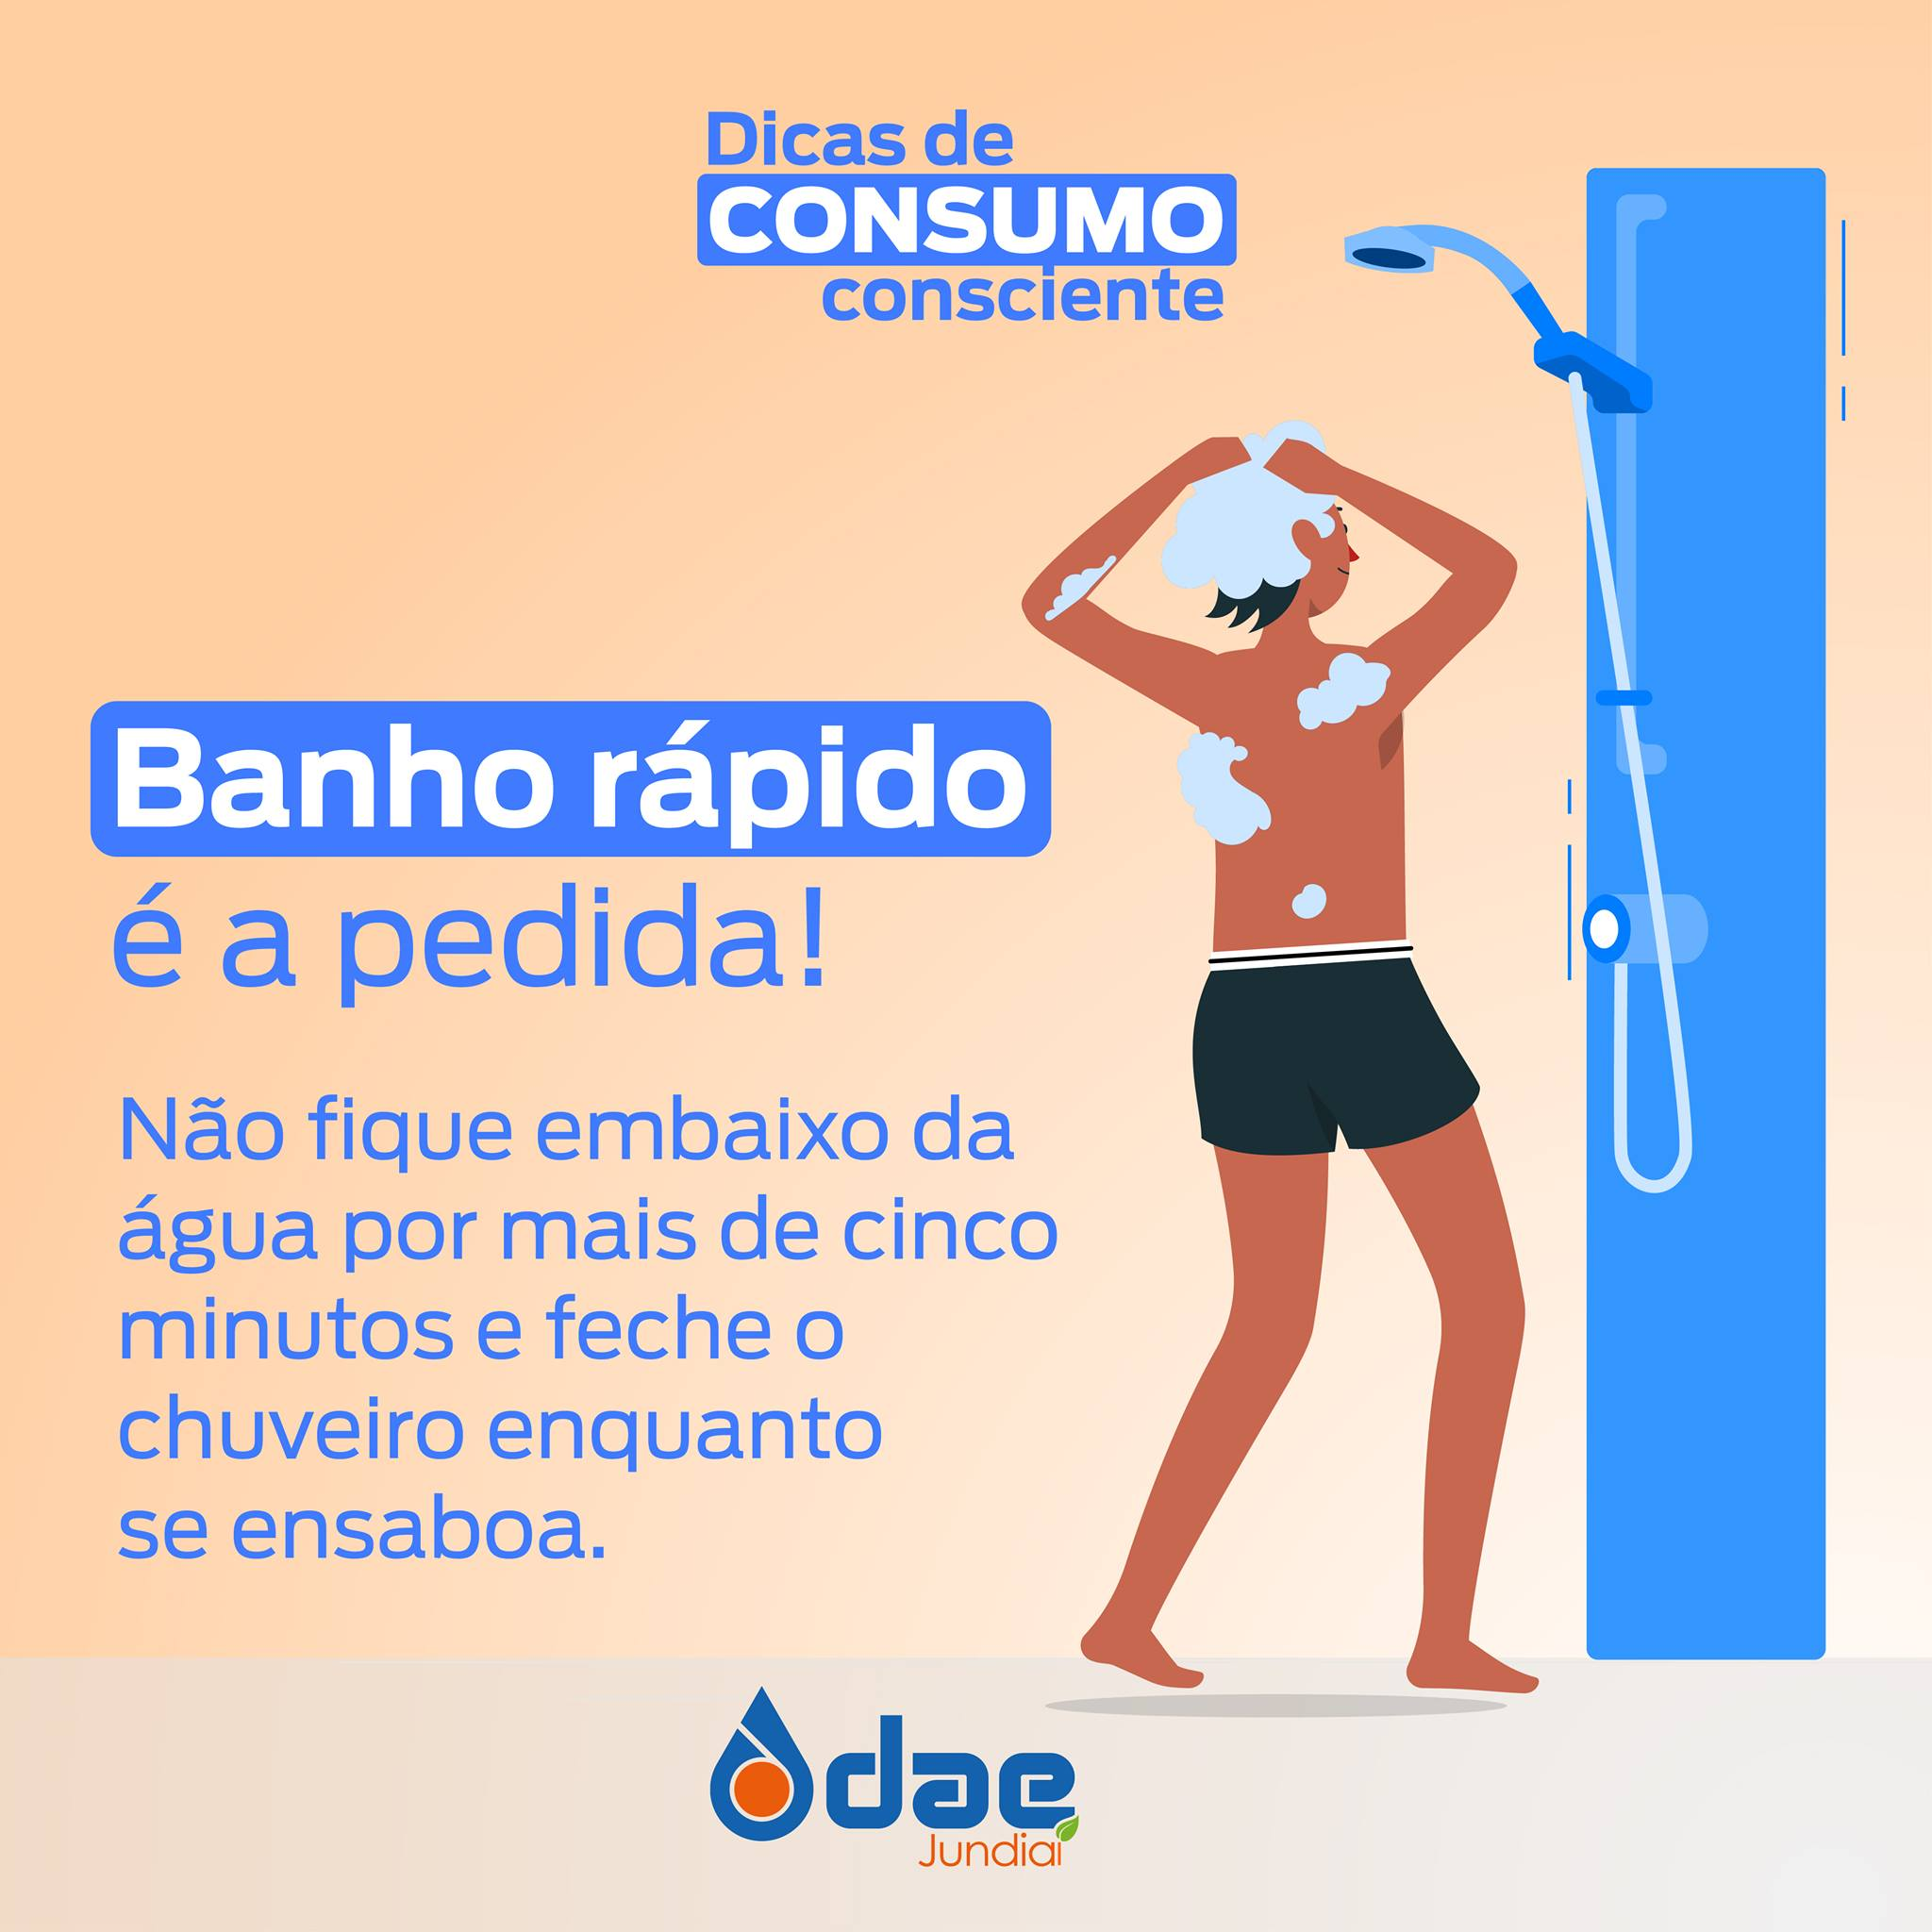
\includegraphics[width=5.90556in,height=5.90556in]{media/image16.jpeg}

\begin{escolha}
\item Qual é o objetivo dessa campanha?

\reduline{É uma campanha para conscientização de economia de água durante o banho.\hfill}

\item Segundo o cartaz, como se pode economizar água durante o banho?

\reduline{Não ficando embaixo do chuveiro por mais de cinco minutos e fechando o
chuveiro enquanto se ensaboa.\hfill}

\item O objetivo desse cartaz é convencer os leitores a repensar ou mudar
de atitude. Você foi convencido? Justifique sua resposta.

\reduline{Resposta pessoal. Aproveite o momento e explique aos alunos que a
economia de água não apenas preserva o ambiente, mas também reflete em
economia financeira, tendo em vista que a conta diminui. Vale lembrar,
ainda, que a água que chega à nossa casa tem um custo de captação,
tratamento e distribuição.\hfill}
\end{escolha}

\colorsec{Treino}

\num{1} Leia o cartaz relacionado à água.
%(Fácil)
%https://www.saopedro.sp.gov.br/saaesp-faz-atividade-especial-para-celebrar-dia-mundial-da-agua
%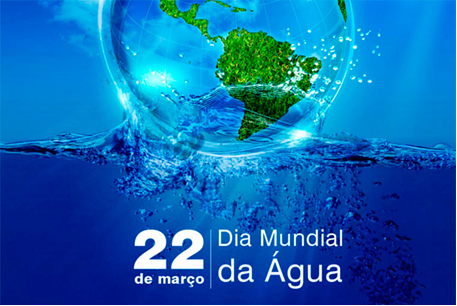
\includegraphics[width=4.75972in,height=3.18681in]{media/image17.png}

\fonte{Disponível em: Prefeitura de São Pedro. Disponível em:
www.saopedro.sp.gov.br/saaesp-faz-atividade-especial-para-celebrar-dia-mundial-da-agua.
Acesso em: 7 mar. 2023.}

A finalidade desse cartaz é

\begin{escolha}
\item incentivar o uso desse recurso natural de todas as formas possíveis.

\item conscientizar sobre o uso de forma econômica e sem desperdícios.

\item conscientizar a população de que este é um recurso natural ilimitado.

\item reconhecer que este é um recurso sem problemas de escassez.
\end{escolha}

\coment{Saeb D4 - Identificar o tema central do texto.

BNCC: EF03LP19: Identificar e discutir o propósito do uso de recursos de
persuasão (cores, imagens, escolha de palavras, jogo de palavras,
tamanho de letras) em textos publicitários e de propaganda, como
elementos de convencimento.}


(A) Incorreta. A água, por ser um recurso finito, deve ser utilizada
apenas quando necessária.

(B) Correta. A imagem apresenta o cartaz que traz a informação sobre o
dia internacional da água. Assim, é possível identificar que a
divulgação dessa data é importante para conscientizar a população de que
este é um recurso finito, isto é, que pode acabar.

(C) Incorreta. A água potável é um recurso finito.

(D) Incorreta. A água é um recurso limitado.

\num{2} Analise a campanha de doação de sangue. (Médio)

%http://www.moreirasales.pr.gov.br/noticia/2203/doe-sangue-salve-vidas-campanha-de-doacao-de-sangue-sera-realizado-na-proxima-semana/
\includegraphics[width=5.90556in,height=5.90556in]{media/image18.jpeg}
%Disponível em: \url{http://www.moreirasales.pr.gov.br/noticia/2203/doe-sangue-salve-vidas-campanha-de-doacao-de-sangue-sera-realizado-na-proxima-semana/}. Acesso em: 7 mar. 2023.

O \emph{slogan} da campanha é

\begin{escolha}
\item ``doe sague, salve vidas''.

\item ``divida o amor que corre nas suas veias''.

\item ``participe da campanha de doação de sangue''.

\item ``Moreira Sales''.
\end{escolha}

\coment{Saeb D6 - Utilizar informações oferecidas por um glossário, verbete de
dicionário ou texto informativo na compreensão ou interpretação do
texto.

BNCC: EF03LP19: Identificar e discutir o propósito do uso de recursos de
persuasão (cores, imagens, escolha de palavras, jogo de palavras,
tamanho de letras) em textos publicitários e de propaganda, como
elementos de convencimento.}

(A) Correta. Slogan é uma pequena frase usada para resumir uma campanha.
No caso da campanha de doação de sangue, o slogan é ``doe sangue, salve
vidas''.

(B) Incorreta. Esse é o título da campanha.

(C) Incorreta. Esse é um subtítulo que introduz as informações sobre
onde e quando doar sangue.

(D) Incorreta. Moreira Sales é a instituição responsável pela veiculação
do anúncio.

\num{3} Leia o cartaz a seguir, observando as imagens e o texto. (Difícil)

%www.saude.pr.gov.br/modules/noticias/article.php?storyid=4950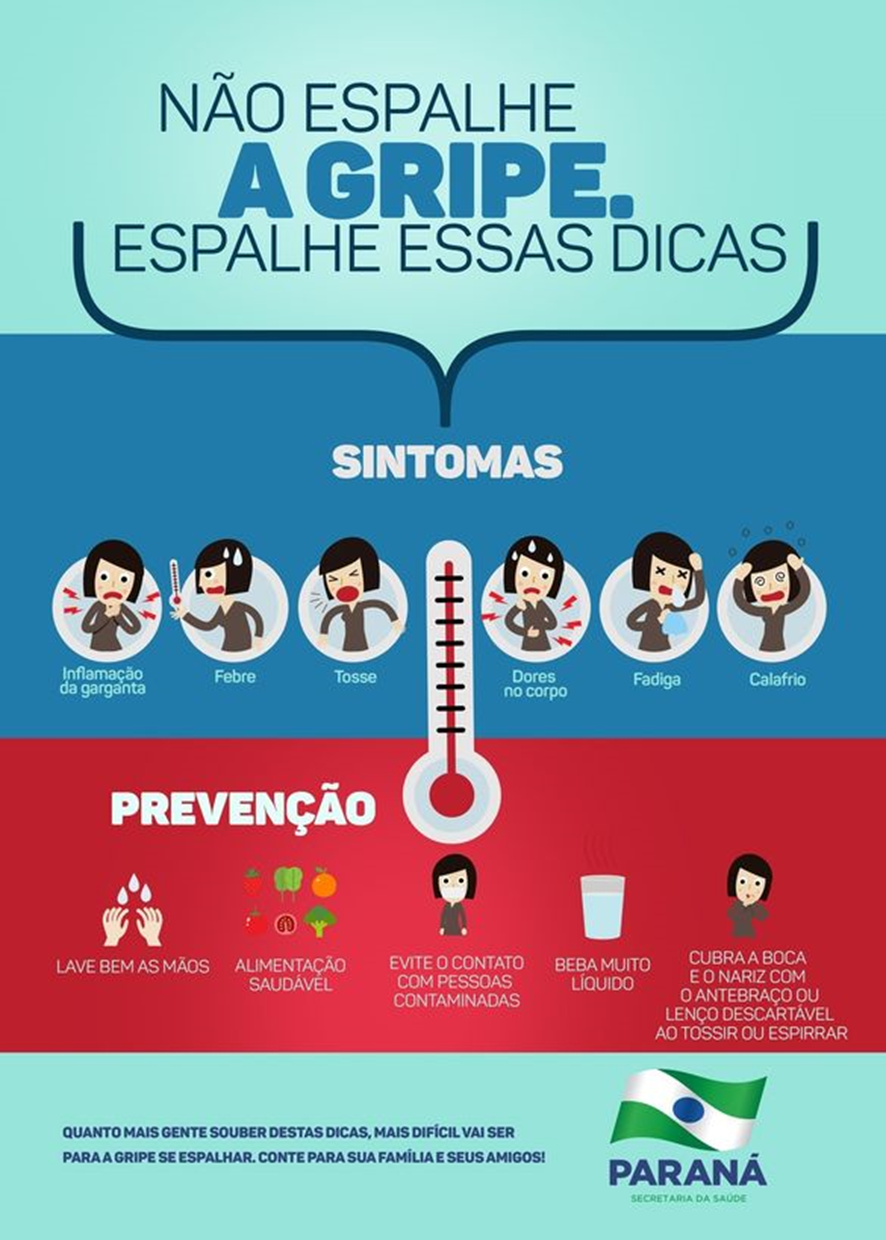
\includegraphics[width=5.90694in,height=8.26736in]{media/image19.png}
%SECRETARIA DA SAÚDE DO PARANÁ. Governo lança campanha para estimular prevenção de gripe. Disponível em: \textless{}www.saude.pr.gov.br/modules/noticias/article.php?storyid=4950\textgreater{}. Acesso em: 7 mar. 2023.

A finalidade dessa campanha é

\begin{escolha}
\item fazer com que as pessoas se alimentem melhor com comidas saudáveis.

\item prevenir que as pessoas passem gripe às outras, apresentando dicas
de como não contrair a doença.

\item informar quais são os sintomas da gripe, de modo que as pessoas
possam combatê-los.

\item apresentar informações sobre como prevenir a gripe e como entender
se houve a contração da doença.
\end{escolha}

\coment{Saeb D9 - Realizar inferências e antecipações em relação ao conteúdo e à
intencionalidade a partir de indicadores como tipo de texto e
características gráficas.

BNCC: EF03LP19: Identificar e discutir o propósito do uso de recursos de
persuasão (cores, imagens, escolha de palavras, jogo de palavras,
tamanho de letras) em textos publicitários e de propaganda, como
elementos de convencimento.}

(A) Incorreta. A finalidade do texto não é essa, uma vez que a
alimentação saudável está relacionada com a prevenção da gripe.

(B) Incorreta. Não há dicas sobre como não contrair a doença, mas dicas
de se prevenir contra ela.

(C) Incorreta. Não há informação de como se podem combater os sintomas
da gripe.

(D) Correta. A campanha tem como finalidade mostrar ao leitor dicas de
quais ações diárias podem prevenir a gripe.

\chapter{Notícias}
\markboth{Módulo 5}{}

\coment{Neste módulo, espera-se que os alunos leiam
e compreendam texto do campo da vida pública; infiram significado de
expressões apresentadas no título do capítulo; identifiquem elementos
apresentados no primeiro parágrafo da notícia (antecipação sobre o
fato); estabeleçam expectativas em relação ao texto a ser lido com base
nos conhecimentos prévios; observem manchetes de jornais e reconhecer
suas características e função no texto.\\
Habilidades BNCC: EF35LP16

\colorsec{Habilidades SAEB}

%https://br.freepik.com/vetores-gratis/pessoas-sem-rosto-com-jornais\_23822995.htm\#page=2\&query=manchete\&position=31\&from\_view=keyword\&track=sph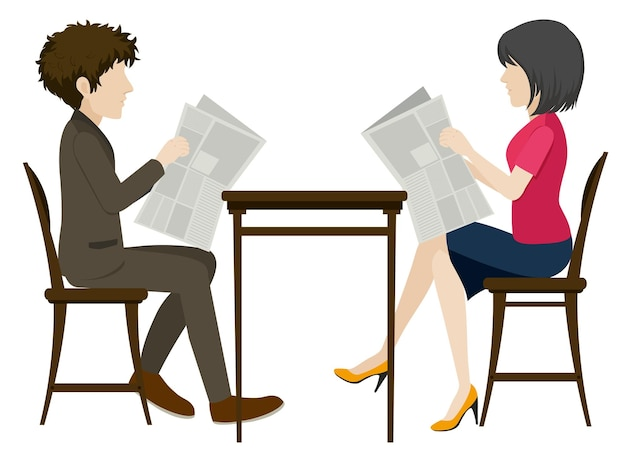
\includegraphics[width=5.41667in,height=3.95422in]{media/image20.jpeg}

\conteudo{
\textbf{NOTÍCIAS}

\textbf{Notícia} consiste em um gênero textual muito presente no
cotidiano das pessoas. Sua finalidade é informar em relação a fatos e
acontecimentos de relevância da atualidade que aconteceram nos mais
variados locais, que normalmente interessam grande parte da população.

As notícias podem ser veiculadas nos meios de comunicação: por meio da
escrita, como são encontradas em jornais e revistas, impressos ou por
meio da fala, como ocorre nos em noticiários da televisão, do rádio e,
também, da internet.

Seja qual for o formato, as notícias costumam ser acompanhadas por
imagens (fotos, mapas, infográficos etc.). De acordo com o público-alvo
ou do assunto a ser abordado, a notícia pode apresentar tanto a
linguagem formal como a informal.

Ao escrever uma notícia, é importante lembrar-se de que seu principal
objetivo é transmitir informações, de modos claro e objetivo, em relação
aos acontecimentos. Assim sendo, é fundamental deixar claro no texto
qual fato é noticiado e com quem, quando, onde, como e por que esse fato
aconteceu.

A notícia apresenta uma estrutura bem definida, que deve conter: título,
lide e corpo da notícia. O título, normalmente, deve ser chamativo e
apresentar os elementos fundamentais que serão relatados na notícia.
}

\colorsec{Atividades}

\num{1} Leia esta notícia.

%07/06/2022

%\href{https://observatorio3setor.org.br/author/maria-fernanda-garcia/}{MARIA FERNANDA GARCIA}~ \href{https://observatorio3setor.org.br/category/noticias/mundo/}{MUNDO}~\href{https://observatorio3setor.org.br/category/noticias/}{NOTÍCIAS}

\begin{quote}
\textbf{Milagre: menino de 4 anos sobrevive sozinho por 2 dias em mata densa e fria}

\emph{Ryker Webb, de 4 anos, foi encontrado após passar dois dias
sozinho em uma área de mata com baixas temperaturas, em Montana, nos
EUA. Segundo as autoridades, cerca de 53 pessoas se empenharam nas
buscas do menino}

Ryker Webb, de 4 anos, foi encontrado após passar dois dias sozinho em
uma área de mata com baixas temperaturas, no estado de Montana, nos
Estados Unidos.

O menino desapareceu na última sexta-feira (03/06) e foi encontrado no
domingo (05/06) após um grande esforço que envolveu equipes de
socorristas, drones, helicópteros e barcos. Quando foi localizado, Webb
estava ileso, mas~``faminto, com sede e frio'', segundo o texto que o
Gabinete do Xerife do Condado de Lincoln publicou em sua página no
Facebook.

As autoridades enviaram um ``código vermelho'' de alerta a todos os
vizinhos da família Webb, pedindo a eles que procurassem a criança em
suas propriedades.

O pequeno Ryker estava brincando com o cachorro de sua família, no
quintal da casa onde mora, quando de repente desapareceu. Ele foi
encontrado a cerca de 3,8 km do local, depois de enfrentar a temperatura
de 4°C e chuvas fortes, que atrapalharam o trabalho das equipes de
resgate.

O Gabinete do Xerife local ainda ressaltou que a vegetação densa da área
tornou a busca ``extremamente difícil''. Quando a criança foi
localizada, 53 pessoas estavam empenhadas no trabalho
de resgate na
região. Autoridades e voluntários consideraram um verdadeiro milagre o
pequeno conseguir sobreviver em um terreno tão hostil com baixas
temperaturas.
\end{quote}

\fonte{GARCIA, Maria Fernanda. Observatório do terceiro setor. Disponível em:
https://observatorio3setor.org.br/noticias/milagre-menino-de-4-anos-sobrevive-sozinho-por-2-dias-em-mata-densa-e-fria/.
Acesso em: 07 mar. 2023.}

\begin{escolha}
\item Que fato é relatado na notícia?

\reduline{É relatado o fato de um menino de 4 anos sobreviver sozinho por 2 dias em mata densa e fria.\hfill}

\item Onde o fato aconteceu?

\reduline{Em Montana, nos EUA.\hfill}

\item Quando o fato aconteceu?

\reduline{O menino desapareceu na última sexta-feira (03/06) e foi encontrado no domingo (05/06)\hfill}

\item
  O que você observou para chegar a essa conclusão?

\reduline{Resposta pessoal.
  Espera-se que os alunos tenham observado a data em que a notícia foi
  publicada e a informação que aparece no segundo parágrafo: ``O menino
  desapareceu na última sexta-feira (03/06) e foi encontrado no domingo
  (05/06)''.\hfill}

\item Quem são os envolvidos no fato?

\reduline{Ryker Webb, equipes de socorristas, autoridades e voluntários.\hfill}

\item Onde a notícia foi publicada?

\reduline{No Observatório do terceiro setor.\hfill}

\item Quem escreveu a notícia?

\reduline{Maria Fernanda Garcia\hfill}

\item Essa notícia foi escrita para quem?

\reduline{Espera-se que os alunos percebam
que a notícia foi publicada para leitores interessados no conteúdo
divulgado.\hfill}

\item Por você acha que esse fato virou notícia?

\reduline{Resposta pessoal.
Espera-se que os alunos percebam que o fato virou notícia porque não é
comum um menino de 4 anos sobreviver sozinho por 2 dias em mata densa e
fria.\hfill}
\end{escolha}

\num{2} Releia o título da notícia e o texto que vem após o título.

\begin{quote}
\textbf{Milagre: menino de 4 anos sobrevive sozinho por 2 dias em mata densa e fria}

\emph{Ryker Webb, de 4 anos, foi encontrado após passar dois dias
sozinho em uma área de mata com baixas temperaturas, em Montana, nos
EUA. Segundo as autoridades, cerca de 53 pessoas se empenharam nas
buscas do menino}
\end{quote}

\begin{escolha}
\item Os títulos dos textos jornalísticos são denominados de \reduline{manchete\hfill}.

\item Qual é a função da manchete? Marque a(s) alternativa(s) correta(s).

\begin{boxlist}
\boxitem[\rosa{X}] Chamar a atenção do leitor para o assunto da notícia.

\boxitem[] Narrar a notícia.

\boxitem[\rosa{X}] Mostrar qual será o assunto tratado.
\end{boxlist}

\item Elabore um novo título para essa notícia.

\reduline{Sugere-se que os alunos
compartilhem as respostas, averiguando a coerência com o tema da
notícia.\hfill}

\colorsec{Treino}

\num{1} Leia o texto a seguir.
%(Fácil)

\begin{quote}
\textbf{Canudo sustentável de bambu ganha adeptos no AC e engenheiro
recebe até 500 encomendas de kits por mês}

O canudo plástico parece inofensivo, mas virou um vilão para o meio
ambiente, porque não é biodegradável e leva centenas de anos para se
decompor. {[}...{]}

Em 2019, o Acre aprovou uma lei --- ainda sem regulamentação ---
proibindo o canudo plástico.

No estado acreano, uma alternativa sustentável, leve, durável, prática e
reutilizável vem ganhando adeptos: o canudo de bambu. Em seis meses, o
agrônomo Emanuel Amaral, que confecciona o canudo, viu a procura pelos
kits aumentar em até 400\%.

{[}...{]}
\end{quote}

\fonte{NASCIMENTO, Aline. ``Canudo sustentável de bambu ganha adeptos no AC e
engenheiro recebe até 500 encomendas de kits por mês''. G1. Disponível
em:
https://g1.globo.com/ac/acre/natureza/amazonia/noticia/2019/12/31/canudo-sustentavel-de-bambu-ganha-adeptos-no-ac-e-engenheiro-recebe-ate-500-encomendas-de-kits-por-mes.ghtml.
Acesso em: 8 mar. 2023.}

O texto pertence ao gênero textual

\begin{escolha}
\item fábula, porque narra as experiências vividas pelo autor do texto no Acre.

\item notícia, porque informa a solução para a substituição do canudo plástico.

\item poema, porque mostra, por meio de versos, uma ação ocorrida no Acre.

\item conto, porque tem uma narrativa sobre a produção de canudos de bambu.
\end{escolha}

\coment{Saeb D7 - Relacionar, na compreensão do texto, informações textuais com
conhecimentos de senso comum.

BNCC: EF35LP16: Identificar e reproduzir, em notícias, manchetes, lides
e corpo de notícias simples para público infantil e cartas de reclamação
(revista infantil), digitais ou impressos, a formatação e diagramação
específica de cada um desses gêneros, inclusive em suas versões orais.}

(A) Incorreta. Não existe narrativa no trecho.

(B) Correta. O trecho apresentado pertence ao gênero textual notícia,
visto que ele informa ao leitor a alternativa sustentável para
substituir o canudo plástico.

(C) Incorreta. O trecho não está escrito em versos, mas em prosa.

(D) Incorreta. Não há uma narrativa sobre a produção dos canudos de
bambu.

\num{2} Leia a notícia a seguir.
%(Médio)

\begin{quote}
\textbf{Defesas curiosas}

Para escapar dos seus inimigos, certos animais e vegetais possuem
maneiras curiosas para se defender. O gambá e o percevejo exalam mau
cheiro para afugentar seus atacantes. O ouriço-do-mar tem espinhos
protetores em volta do corpo. O polvo solta uma tinta que escurece a
água, facilitando assim a sua fuga. O cacto também tem espinhos
protetores. As flores do açafrão são parecidas com as de outra planta
chamada cólquico que, por ser venenosa, é evitada como alimento por
certos animais. Por causa dessa semelhança, o açafrão fica protegido
também.
\end{quote}

\fonte{ABREU, Ana Rosa et al. Defesas curiosas. Disponível em:
www.dominiopublico.gov.br/download/texto/me000590.pdf. Acesso em: 8 mar.
2023.}

A notícia apresentada não é ficcional porque essa tem

\begin{escolha}
\item manchete e um assunto sobre a realidade.

\item narração para contar um fato que aconteceu recentemente.

\item informações inventadas ou contém elementos fictícios.

\item informações reais que aconteceram recentemente.
\end{escolha}

\fonte{Saeb D2 - Inferir uma afirmação implícita num texto.

BNCC: EF35LP16: Identificar e reproduzir, em notícias, manchetes, lides
e corpo de notícias simples para público infantil e cartas de reclamação
(revista infantil), digitais ou impressos, a formatação e diagramação
específica de cada um desses gêneros, inclusive em suas versões orais.}

(A) Incorreta. A notícia ficcional não apresenta fatos reais.

(B) Incorreta. Uma notícia ficcional não é narrativa, mas informativa.

(C) Correta. Notícias ficcionais apresentam informações ou elementos fictícios.

(D) Incorreta. Refere-se à descrição de uma notícia.

\num{3} O texto a seguir traz informações sobre uma competição esportiva. Leia-o atentamente.

\begin{quote}
\textbf{Seleção masculina de vôlei estreia hoje na Liga das Nações}

{[}...{]} A seleção masculina de voleibol estreia nesta sexta-feira
(31), na Liga das Nações,

jogando em Katowice, na Polônia, contra a seleção dos Estados Unidos.
Esta é a primeira

etapa de cinco envolvendo 16 equipes. No grupo de Katowice estão Brasil,
Estados Unidos, Austrália e Polônia. Todos as 16 seleções jogam entre si
e em cada etapa mudam os adversários e a cidade sede. {[}...{]}
\end{quote}

\fonte{TAVARES, Eurico. Seleção masculina de vôlei estreia hoje na Liga das
Nações. Rádioagência Nacional. Disponível em:
http://radioagencianacional.ebc.com.br/geral/audio/2019-05/selecao-masculina-de-volei-estreia-hoje-na-liga-das-nacoes.
Acesso em: 8 mar. 2023.}

Com base nas características apresentadas, percebe-se que o texto consiste no gênero

\begin{escolha}
\item entrevista.

\item notícia.

\item diário.

\item conto.
\end{escolha}

\coment{Saeb D4 - Identificar o tema central do texto.

BNCC: EF35LP16: Identificar e reproduzir, em notícias, manchetes, lides
e corpo de notícias simples para público infantil e cartas de reclamação
(revista infantil), digitais ou impressos, a formatação e diagramação
específica de cada um desses gêneros, inclusive em suas versões orais.}

(A) Incorreta. O trecho apresentado não faz parte de uma entrevista.

(B) Correta. O texto a seguir faz parte do gênero notícia por relatar um
fato e apresentar informações em relação a ele.

(C) Incorreta. O trecho apresentado não faz parte de um diário.

(D) Incorreta. O trecho apresentado não faz parte de um conto.

\chapter{Módulo 6}
\markboth{Módulo 6}{}

\coment{Neste módulo, os alunos vão reconhecer os efeitos dos verbos de
enunciação no discurso direto, percebendo a importância desses verbos
para indicar os turnos de fala dos diálogos e para especificar
entonações e sentidos das falas das personagens.}

\conteudo{
\textbf{Verbos de enunciação e variedades linguísticas no discurso direto}

%https://pixabay.com/pt/illustrations/gabarito-relat\%c3\%b3rio-de-volta-3387220/
\includegraphics[width=5.01488in,height=3.34306in]{media/image21.png}

Na língua portuguesa, há palavras que anunciam quando um personagem vai falar e o modo como vai falar, por exemplo: ``disse'', ``perguntou'', ``respondeu''.

Observe este exemplo:

\begin{quote}
--- Eu não disse? Ele sempre volta! --- \textbf{disse} o dono do cachorro.
\end{quote}

Essas palavras podem ser encontradas antes, no meio ou depois das falas
da personagem e são chamados de verbos de enunciação/elocução. Estes são
verbos utilizados no texto que servem para introduzir/iniciar a fala dos
personagens, indicando suas atitudes e ações. Além disso, podemos
observar também, que as falas das personagens podem ser introduzidas
seguidas de dois pontos e travessão, em forma de diálogo. Esses
elementos são importantes, pois nos ajudam a compreender o jeito de
falar dos personagens, a intencionalidade e como a frase foi falada.

Agora, vamos treinar!
}

\colorsec{Atividades}

\num{1} Leia o texto a seguir.

%https://pixabay.com/pt/illustrations/lobo-fera-lobo-cinza-animal-6612744/
%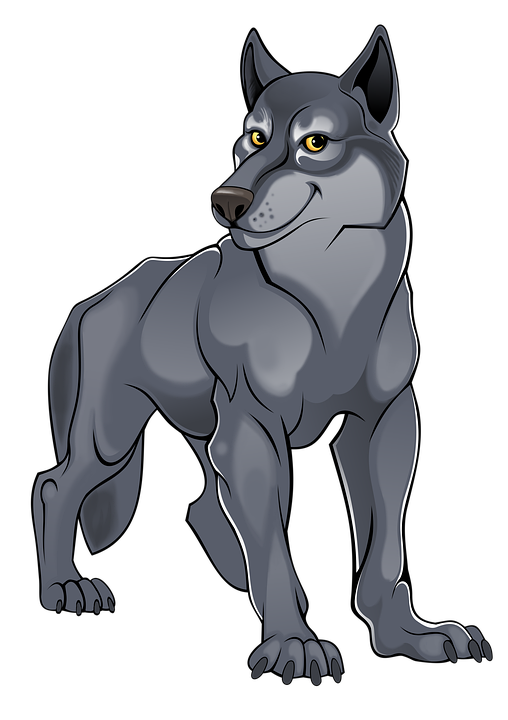
\includegraphics[width=2.69792in,height=3.82382in]{media/image22.png}

\begin{quote}
\textbf{O LOBO E O CÃO}

Um lobo e um cão se encontraram num caminho. Disse o lobo:

L--- Companheiro, você está com ótimo aspecto: gordo, o pelo
lustroso\ldots{} Estou até com inveja!

C--- Ora, faça como eu --- respondeu o cão. --- Arranje um bom amo. Eu
tenho comida na hora certa, sou bem tratado\ldots{} Minha única
obrigação é latir à noite, quando aparecem ladrões. Venha comigo e você
terá o mesmo tratamento.

O lobo achou ótima a ideia e se puseram a caminho.

L Mas, de repente, o lobo reparou numa coisa. --- O que é isso no seu
pescoço, amigo? Parece um pouco esfolado\ldots{} --- observou ele.

C --- Bem --- disse o cão --- isso é da coleira. Sabe? Durante o dia,
meu amo me prende com uma coleira, que é para eu não assustar as pessoas
que vêm visitá-lo.

O lobo se despediu do amigo ali mesmo:

L --- Vamos esquecer --- disse ele. --- Prefiro minha liberdade à sua
fartura.
\end{quote}

\fonte{\textbf{O LOBO e o cão.} Disponível em:
http://www.dominiopublico.gov.br/download/texto/me000589.pdf. Acesso em:
9 mar. 2023.}

\begin{tabular}{ll}
\textbf{Glossário} & \mbox{}\\
Amo & dono do cão\\
Cativo & preso\\
Esfolado & machucado\\
Lustroso & brilhante\\
\end{tabular}

\begin{escolha}
\item Quem são as personagens da história?

\reduline{O cão e o lobo.\hfill}

\item O texto que você acabou de ler é do gênero:

\begin{boxlist}
\boxitem[] diário, em que uma~pessoa~relata experiências.

\boxitem[\rosa{X}] fábula, que traz uma pequena história com ensinamento moral.

\boxitem[] notícia, que veicula um acontecimento real para o grande público.
\end{boxlist}

\item Qual convite o lobo recebeu do cão?

\reduline{O cão convidou o lobo a viver com ele.\hfill}

\item Por que o lobo desistiu do convite?

\reduline{Ele desistiu depois de ver as marcas da ``coleira'' no pescoço do cão.\hfill}

\item Descreva o conflito principal da fábula.

\reduline{O principal conflito ocorre entre o lobo melhorar de vida ou perder a liberdade.\hfill}
\end{escolha}

\num{2} Quem conta a história \textbf{O lobo e o cão}? Assinale a alternativa correta.

\begin{boxlist}
\boxitem[] Um narrador que participa da história (narração em 1ª pessoa).

\boxitem[\rosa{X}] Um narrador que não participa das ações (narração em 3ª pessoa).
\end{boxlist}

\num{3} Neste trecho, quem está participando do diálogo?

\begin{quote}
--- Companheiro, você está com ótimo aspecto: gordo, o pelo
lustroso\ldots{} Estou até com inveja!

--- Ora, faça como eu --- respondeu o cão. --- Arranje um bom amo. Eu
tenho comida na hora certa, sou bem tratado\ldots{} Minha única
obrigação é latir à noite, quando aparecem ladrões. Venha comigo e você
terá o mesmo tratamento.
\end{quote}

\reduline{ O cão e o lobo.\hfill}

\num{4} Como ficaria a história se o diálogo fosse composto apenas pelas falas
das personagens, sem a intervenção do narrador?

\reduline{Resposta pessoal.
Espera-se que percebam que o leitor não saberia de que maneira as
personagens falaram pois não haveria os comentários, nem os verbos de
enunciação.\hfill}

\reduline{Explique aos alunos que, em algumas narrativas, pode acontecer de o
narrador não indicar quem fala; a identificação é feita pela sequência
do discurso e a apresentação pelos verbos de enunciação.\hfill}

\num{5} Releia a fábula e pinte no texto:

\begin{itemize}
\item de azul as falas do cão;

\item de verde as falas do lobo.
\end{itemize}

\coment{As respostas estão indicadas no texto com as letras C (cão) e L (lobo).}

6. Qual o efeito expresso pelo discurso direto na fábula ``\textbf{O
lobo e o cão''}?

\reduline{Espera-se que percebam que o discurso direto apresenta
ao leitor a conversa das personagens como se estivesse ocorrendo naquele
momento.\hfill}

\colorsec{Treino}

\num{1} Leia o trecho do conto ``Água da vida'', verificando o modo das falas.

%(Fácil)

\begin{quote}
\textbf{Água da vida}

Houve, uma vez, um rei muito poderoso, que vivia feliz e tranquilo em
seu reino. Um belo dia, adoeceu gravemente e ninguém tinha esperanças de
que escapasse. Ele tinha três filhos, {[}...{]}.

Encontravam-se eles no jardim do castelo a chorar e, de repente, viram
surgir à sua frente um velho de aspecto venerável, que indagou a causa
de tamanha tristeza. Disseram-lhe que estavam aflitos porque o pai
estava gravemente enfermo e os médicos já não tinham esperanças de o
salvar.

O velho, então, disse-lhe:

- Eu conheço um remédio muito eficaz, que poderá curá-lo; é a famosa
Água da Vida. Mas é muito difícil obtê-la.
\end{quote}

\fonte{GRIMM. A água da vida. Disponível em:
https://www.grimmstories.com/pt/grimm\_contos/a\_agua\_da\_vida. Acesso
em: 9 mar. 2023.}

O trecho ``- Eu conheço um remédio muito eficaz, que poderá curá-lo; é a
famosa Água da Vida. Mas é muito difícil obtê-la'' está em discurso

\begin{escolha}
\item direto, porque é a fala do personagem separada por travessão.

\item indireto, porque é a fala do personagem por meio do narrador.

\item direto, porque é a transcrição da fala do próprio narrador do conto.

\item indireto, porque apresenta a introdução do narrador ``disse-lhe''.
\end{escolha}

\coment{Saeb D7 - Relacionar, na compreensão do texto, informações textuais com
conhecimentos de senso comum.

BNCC EF35LP22: Perceber diálogos em textos narrativos, observando o
efeito de sentido de verbos de enunciação e, se for o caso, o uso de
variedades linguísticas no discurso direto.}

(A) Correta. O trecho apresentado é a fala direta do personagem
denominado como ``velho'', como se vê pela separação feita pelos dois
pontos e travessão.

(B) Incorreta. O trecho apresenta uma fala direta; o discurso indireto
pode ser visto no conto no trecho ``Disseram-lhe que estavam aflitos
porque o pai estava gravemente enfermo e os médicos já não tinham
esperanças de o salvar''.

(C) Incorreta. A fala é introduzida como ``O velho, então, disse-lhe'',
mostrando que é a fala do personagem ``velho''.

(D) Incorreta. O verbo de elocução é seguido pelos dois pontos e pelo
travessão, o que mostra uma separação entre o discurso do narrador e a
fala do personagem, caracterizando como discurso direto.

\num{2} O diálogo a seguir faz parte do livro O mágico de Oz e mostra a
personagem Dorothy e a Bruxa do Norte conversando.

%(Médio) 

\begin{quote}
{[}...{]}

― Eu sempre acreditei que todas as bruxas fossem más ― disse a menina,
que sentia medo

por estar frente a frente com uma bruxa de verdade.

― Oh, não, não, isso é um erro! Havia quatro bruxas na Terra de Oz: as
que vivem no Norte e no Sul são boas, as do Leste e do Oeste eram bruxas
malvadas, mas agora que você matou uma delas sobrou apenas uma bruxa má
em toda a Terra de Oz: a que vive no Reino do Oeste.

Depois de pensar um pouco, Dorothy disse:

― Mas a tia Ema me contou que todas as bruxas morreram há muitos e
muitos anos.

― Quem é a tia Ema? ― perguntou a bruxinha.

― É a minha tia que mora no Kansas, eu vim de lá.
\end{quote}

\fonte{BAUM, Frank L. O mundo mágico de OZ. Disponível em:
www.dominiopublico.gov.br/download/texto/ph000102.pdf. Acesso em: 9 mar.
2023.}

No trecho ``― Oh, não, não, isso é um erro!'', o uso de ``oh'' indica

\begin{escolha}
\item alegria.

\item surpresa.

\item alívio.

\item tristeza.
\end{escolha}

\coment{Saeb D18 -- Reconhecer o efeito
de sentido decorrente da escolha de uma determinada palavra ou
expressão.

BNCC EF35LP30 - Diferenciar discurso indireto e discurso direto,
determinando o efeito de sentido de verbos de enunciação e explicando o
uso de variedades linguísticas no discurso direto, quando for o caso.}

(A) Incorreta. Conforme o contexto da oração, a bruxa usa a expressão
para mostrar espanto.

(B) Correta. Interjeições são palavras utilizadas para expressar emoções
e variam muito conforme o contexto. Normalmente, apresentam-se em
diálogos e são classificadas de acordo com o sentimento expresso.

(C) Incorreta. Normalmente, para indicar alívio, são utilizadas
expressões como ``ufa'' e ``ah''.

(D) Incorreta. A interjeição indicaria tristeza caso a bruxa se
lamentasse para Dorothy.

\num{3} O livro Viagem ao centro da Terra, escrito por Júlio Verne e
publicado em 1864, é o relato do jovem Axel sobre a jornada que
percorreu com o seu tio. O diálogo a seguir refere-se a uma discussão
acerca da continuidade da expedição.
%(Difícil) 

\begin{quote}
{[}...{]}

--- Oh, não tenho medo de que o céu nos caia sobre a cabeça. Agora, meu
tio, quais são seus planos? O senhor não está pensando em voltar à
superfície do globo?

--- Voltar? Ora essa! Muito pelo contrário, pretendo continuar a viagem
já que tudo correu tão bem até aqui.

--- É que não vejo como atravessaremos essa planície líquida.

--- Não pretendo mergulhar de cabeça.
\end{quote}

\fonte{VERNE, Júlio. \textbf{Viagem ao centro da Terra}. Disponível em:
www.ebc.com.br/sites/\_portalebc2014/files/atoms/files/viagem\_ao\_centro\_da\_terra\_\_julio\_verne.pdf.
Acesso em: 9 mar. 2023.}

O trecho apresenta um diálogo entre tio e sobrinho que utiliza

\begin{escolha}
\item a norma popular.

\item as variedades linguísticas.

\item a linguagem científica.

\item a norma-padrão.
\end{escolha}

\coment{Saeb D27 - Identificar características típicas da fala em um texto
escrito.

BNCC EF35LP30 - Diferenciar discurso indireto e discurso direto,
determinando o efeito de sentido de verbos de enunciação e explicando o
uso de variedades linguísticas no discurso direto, quando for o caso.}

(A) Incorreta. O texto segue a norma-padrão da língua.

(B) Incorreta. O texto segue a norma-padrão da língua. Não há variações linguísticas.

(C) Incorreta. Não utilizam linguagem científica.

(D) Correta. O trecho apresentado está seguindo a norma-padrão da língua.

\chapter{Concordância nominal}
\markboth{Módulo 7}{}

\begin{quote}
Neste módulo, os alunos vão identificar adjetivos no texto e os
substantivos a que se referem; perceber a concordância em número e
gênero entre artigo, substantivo e adjetivo; aplicar a concordância
nominal nos diversos contextos para a escrita correta.
\end{quote}

\subsection{Conteúdo}\label{conteuxfado-6}

\begin{quote}
\textbf{CONCORDÂNCIA NOMINAL}

https://pixabay.com/pt/illustrations/abc-alfabeto-letras-ler-aprender-916665/


\includegraphics[width=4.16597in,height=2.95939in]{media/image23.png}

Imagine a confusão que seria a comunicação se as pessoas ou os objetos
não tivessem nomes para identificá-los?~

\textbf{Substantivo} é o nome de cada coisa que existe no planeta. Há
variadas formas de classificar um substantivo: por exemplo, uma camiseta
pode ser de algodão, em relação ao tecido, em relação à cor, pode ser
branca, preta, colorida, etc.; no tamanho, pode ser curta ou comprida. E
também podemos dizer que ela está barata ou cara, em relação ao preço!
Essas características que podemos dar a um substantivo chamamos de
\textbf{adjetivos}, que são palavras que modificam o significado do
substantivo, acrescentando-lhe noções de qualidade, natureza, estado
etc.

Importante saber que o \textbf{substantivo} pode variar em
\textbf{gênero} (masculino ou feminino) e \textbf{número} (singular ou
plural). O \textbf{adjetivo} e o \textbf{artigo} devem concordar em
gênero e número com o substantivo a que se referem.
\end{quote}

\colorsec{Atividades}

\begin{quote}
Conto é um gênero narrativo muito popular na literatura. Sua principal
característica é ter uma estrutura com início, meio e fim, mas o
desenvolvimento acontece de forma breve.

Chame a atenção dos alunos para o título do texto: ``O soldadinho de
chumbo''. Peça a eles que levantem hipóteses sobre o enredo com base no
título. Provavelmente, alguns farão referência a um enredo de conto de
fadas. Incentive a participação dos alunos.
\end{quote}

\num{1}

\begin{quote}
Leia o conto Joãozinho-sem-medo e, em seguida, responda às questões
propostas.

\textbf{O SOLDADINHO DE CHUMBO}

https://br.freepik.com/vetores-gratis/guarda-em-pe-com-uma-arma\_13571969.htm\#query=soldadinho\%20chumbo\&position=3\&from\_view=search\&track=ais


\includegraphics[width=2.68750in,height=4.34722in]{media/image24.jpeg}

Numa loja de brinquedos havia uma caixa de papelão com vinte e cinco
soldadinhos de chumbo, todos iguaizinhos, pois haviam sido feitos com o
mesmo molde. Apenas um deles era perneta: como fora o último a ser
fundido, faltou chumbo para completar a outra perna. Mas o soldadinho
perneta logo aprendeu a ficar em pé sobre a única perna e não fazia feio
ao lado dos irmãos.

Esses soldadinhos de chumbo eram muito bonitos e elegantes, cada qual
com seu fuzil ao ombro, a túnica escarlate, calça azul e uma bela pluma
no chapéu. Além disso, tinham feições de soldados corajosos e
cumpridores do dever.

Os valorosos soldadinhos de chumbo aguardavam o momento em que passariam
a pertencer a algum menino.

Chegou o dia em que a caixa foi dada de presente de aniversário a um
garoto. Foi o presente de que ele mais gostou:

--- Que lindos soldadinhos! --- exclamou maravilhado.

E os colocou enfileirados sobre a mesa, ao lado dos outros brinquedos. O
soldadinho de uma perna só era o último da fileira.

Ao lado do pelotão de chumbo se erguia um lindo castelo de papelão, um
bosque de árvores verdinhas e, em frente, havia um pequeno lago feito de
um pedaço de espelho.

A maior beleza, porém, era uma jovem que estava em pé na porta do
castelo. Ela também era de papel, mas vestia uma saia de tule bem
franzida e uma blusa bem justa. Seu lindo rostinho era emoldurado por
longos cabelos negros, presos por uma tiara enfeitada com uma pequenina
pedra azul.

A atraente jovem era uma bailarina, por isso mantinha os braços erguidos
em arco sobre a cabeça. Com uma das pernas dobrada para trás, tão
dobrada, mas tão dobrada, que acabava escondida pela saia de tule.

O soldadinho a olhou longamente e logo se apaixonou, e pensando que, tal
como ele, aquela jovem tão linda tivesse uma perna só.

``Mas é claro que ela não vai me querer para marido'', pensou
entristecido o soldadinho, suspirando. ``Tão elegante, tão
bonita\ldots{} Deve ser uma princesa. E eu? Nem cabo sou, vivo numa
caixa de papelão, junto com meus vinte e quatro

irmãos''.

À noite, antes de deitar, o menino guardou os soldadinhos na caixa, mas
não percebeu que aquele de uma perna só caíra atrás de uma grande
cigarreira.

Quando os ponteiros do relógio marcaram meia-noite, todos os brinquedos
se animaram e começaram a aprontar mil e uma. Uma enorme bagunça!

As bonecas organizaram um baile, enquanto o giz da lousa desenhava
bonequinhos nas paredes. Os soldadinhos de chumbo, fechados na caixa,
golpeavam a tampa para sair e participar da festa, mas continuavam
prisioneiros.

Mas o soldadinho de uma perna só e a bailarina não saíram do lugar em
que haviam sido colocados. Ele não conseguia parar de olhar aquela
maravilhosa criatura. Queria ao menos tentar conhecê-la, para ficarem
amigos.

De repente, se ergueu da cigarreira um homenzinho muito mal-encarado.
Era um gênio ruim, que só vivia pensando em maldades. Assim que ele
apareceu, todos os brinquedos pararam amedrontados, pois já sabiam de
quem se tratava.

O geniozinho olhou a sua volta e viu o soldadinho, deitado atrás da
cigarreira.

--- Ei, você aí, por que não está na caixa, com seus irmãos? --- gritou
o monstrinho.

Fingindo não escutar, o soldadinho continuou imóvel, sem desviar os
olhos da bailarina.

--- Amanhã vou dar um jeito em você, você vai ver!

--- Gritou o geniozinho enfezado. --- Pode esperar.

Depois disso, pulou de cabeça na cigarreira, levantando uma nuvem que
fez todos espirrarem.

Na manhã seguinte, o menino tirou os soldadinhos de chumbo da caixa,
recolheu aquele de uma perna só, que estava caído atrás da cigarreira, e
os arrumou perto da janela. O soldadinho de uma perna só, como de
costume, era o último da fila.

De repente, a janela se abriu, batendo fortemente as venezianas. Teria
sido o vento, ou o geniozinho maldoso? E o pobre soldadinho caiu de
cabeça na rua.

O menino viu quando o brinquedo caiu pela janela e foi correndo
procurá-lo na rua. Mas não o encontrou. Logo se consolou: afinal, tinha
ainda os outros soldadinhos, e todos com duas pernas.

Para piorar a situação, caiu um verdadeiro temporal. Quando a tempestade
foi cessando, e o céu limpou um pouco, chegaram dois moleques. Eles se
divertiam, pisando com os pés descalços nas poças de água. Um deles viu
o soldadinho de chumbo e exclamou:

--- Olhe! Um soldadinho! Será que alguém jogou fora porque ele está
quebrado?

--- É, está um pouco amassado. Deve ter vindo com a enxurrada.

--- Não, ele está só um pouco sujo.

--- O que nós vamos fazer com um soldadinho só?

Precisaríamos pelo menos meia dúzia, para organizar uma batalha.

--- Sabe de uma coisa? --- Disse o primeiro garoto. ---

Vamos colocá-lo num barco e mandá-lo dar a volta ao mundo.

E assim foi. Construíram um barquinho com uma folha de jornal, colocaram
o soldadinho dentro dele e soltaram o barco para navegar na água que
corria pela sarjeta.

Apoiado em sua única perna, com o fuzil ao ombro, o soldadinho de chumbo
procurava manter o equilíbrio. O barquinho dava saltos e esbarrões na
água lamacenta, acompanhado pelos olhares dos dois moleques que,
entusiasmados com a nova brincadeira, corriam pela calçada ao lado.

Lá pelas tantas, o barquinho foi jogado para dentro de um bueiro e
continuou seu caminho, agora subterrâneo, em uma imensa escuridão. Com o
coração batendo fortemente, o soldadinho voltava todos seus pensamentos
para a bailarina, que talvez nunca mais pudesse ver.

De repente, viu chegar em sua direção um enorme rato de esgoto, olhos
fosforescente e um horrível rabo fino e comprido, que foi logo
perguntando:

--- Você tem autorização para navegar? Então? Ande, mostre-a logo, sem
discutir.

O soldadinho não respondeu, e o barquinho continuou seu incerto caminho,
arrastado pela correnteza. Os gritos do rato do esgoto exigindo a
autorização foram ficando cada vez mais distantes.

Enfim, o soldadinho viu ao longe uma luz, e respirou aliviado; aquela
viagem no escuro não o agradava nem um pouco. Mal sabia ele que,
infelizmente, seus problemas não haviam acabado.

A água do esgoto chegara a um rio, com um grande salto; rapidamente, as
águas agitadas viraram o frágil barquinho de papel.

O barquinho virou, e o soldadinho de chumbo afundou. Mal tinha chegado
ao fundo, apareceu um enorme peixe que, abrindo a boca, engoliu-o.

O soldadinho se viu novamente numa imensa escuridão, espremido no
estômago do peixe. E não deixava de pensar em sua amada: ``O que estará
fazendo agora sua linda bailarina? Será que ainda se lembra de mim?''.

E, se não fosse tão destemido, teria chorado lágrimas de chumbo, pois
seu coração sofria de paixão.

Passou-se muito tempo --- quem poderia dizer quanto?

E, de repente, a escuridão desapareceu e ele ouviu quando

falavam:

--- Olhe! O soldadinho de chumbo que caiu da janela!

Sabem o que aconteceu? O peixe havia sido fisgado por um pescador,
levado ao mercado e vendido a uma cozinheira. E, por cúmulo da
coincidência, não era qualquer cozinheira, mas sim a que trabalhava na
casa do menino que ganhara o soldadinho no aniversário. Ao limpar o
peixe, a cozinheira encontrara dentro dele o soldadinho, do qual se
lembrava muito bem, por causa daquela única perna.

Levou-o para o garotinho, que fez a maior festa ao revê-lo. Lavou-o com
água e sabão, para tirar o fedor de peixe, e endireitou a ponta do
fuzil, que amassara um pouco durante aquela aventura.

Limpinho e lustroso, o soldadinho foi colocado sobre a mesma mesa em que
estava antes de voar pela janela. Nada estava mudado. O castelo de
papel, o pequeno bosque de árvores muito verdes, o lago reluzente feito
de espelho. E, na porta do castelo, lá estava ela, a bailarina: sobre
uma perna só, com os braços erguidos acima da cabeça, mais bela do que
nunca.

O soldadinho olhou para a bailarina, ainda mais apaixonado, ela olhou
para ele, mas não trocaram palavra alguma. Ele desejava conversar, mas
não ousava. Sentia-se feliz apenas por estar novamente perto dela e
poder amá-la.

Se pudesse, ele contaria toda sua aventura; com certeza a linda
bailarina iria apreciar sua coragem. Quem sabe, até se casaria com
ele\ldots{}

Enquanto o soldadinho pensava em tudo isso, o garotinho brincava
tranquilo com o pião. De repente como foi, como não foi --- é caso de se
pensar se o geniozinho ruim da cigarreira não metera seu nariz ---, o
garotinho agarrou o soldadinho de chumbo e atirou-o na lareira, onde o
fogo ardia intensamente.

O pobre soldadinho viu a luz intensa e sentiu um forte calor. A única
perna estava amolecendo e a ponta do fuzil envergava para o lado. As
belas cores do uniforme, o vermelho escarlate da túnica e o azul da
calça perdiam suas tonalidades.

O soldadinho lançou um último olhar para a bailarina, que retribuiu com
silêncio e tristeza. Ele sentiu então que seu coração de chumbo começava
a derreter --- não só pelo calor, mas principalmente pelo amor que ardia
nele.

Naquele momento, a porta escancarou-se com violência, e uma rajada de
vento fez voar a bailarina de papel diretamente para a lareira, bem
junto ao soldadinho. Bastou uma labareda e ela desapareceu. O soldadinho
também se dissolveu completamente.

No dia seguinte. a arrumadeira, ao limpar a lareira, encontrou no meio
das cinzas um pequenino coração de chumbo: era tudo que restara do
soldadinho, fiel até o último instante ao seu grande amor.

Da pequena bailarina de papel só restou a minúscula pedra azul da tiara,
que antes brilhava em seus longos cabelos negros.

Disponível em:

http://www.dominiopublico.gov.br/download/texto/me000589.pdf. Acesso em:
13 mar. 2023.

a) Qual é o tema tratado no conto?
\protect\hypertarget{_Hlk127887290}{}{}O conto trata de um soldado que
se perdeu da coleção de um menino.

\_\_\_\_\_\_\_\_\_\_\_\_\_\_\_\_\_\_\_\_\_\_\_\_\_\_\_\_\_\_\_\_\_\_\_\_\_\_\_\_\_\_\_\_\_\_\_\_\_\_\_\_\_\_\_\_\_\_\_\_\_\_\_\_

\_\_\_\_\_\_\_\_\_\_\_\_\_\_\_\_\_\_\_\_\_\_\_\_\_\_\_\_\_\_\_\_\_\_\_\_\_\_\_\_\_\_\_\_\_\_\_\_\_\_\_\_\_\_\_\_\_\_\_\_\_\_\_\_

\_\_\_\_\_\_\_\_\_\_\_\_\_\_\_\_\_\_\_\_\_\_\_\_\_\_\_\_\_\_\_\_\_\_\_\_\_\_\_\_\_\_\_\_\_\_\_\_\_\_\_\_\_\_\_\_\_\_\_\_\_\_\_\_

\_\_\_\_\_\_\_\_\_\_\_\_\_\_\_\_\_\_\_\_\_\_\_\_\_\_\_\_\_\_\_\_\_\_\_\_\_\_\_\_\_\_\_\_\_\_\_\_\_\_\_\_\_\_\_\_\_\_\_\_\_\_\_\_

b) Onde inicia a história? Inicia em uma loja de brinquedos.

\_\_\_\_\_\_\_\_\_\_\_\_\_\_\_\_\_\_\_\_\_\_\_\_\_\_\_\_\_\_\_\_\_\_\_\_\_\_\_\_\_\_\_\_\_\_\_\_\_\_\_\_\_\_\_\_\_\_\_\_\_\_\_\_

\_\_\_\_\_\_\_\_\_\_\_\_\_\_\_\_\_\_\_\_\_\_\_\_\_\_\_\_\_\_\_\_\_\_\_\_\_\_\_\_\_\_\_\_\_\_\_\_\_\_\_\_\_\_\_\_\_\_\_\_\_\_\_\_
\end{quote}

\begin{enumerate}
\def\labelenumi{\alph{enumi})}
\item
  Qual foi o motivo de o Soldadinho cair da janela? ~O menino estava
  arrumando os soldadinhos e deixou cair na rua.
\end{enumerate}

\begin{quote}
\_\_\_\_\_\_\_\_\_\_\_\_\_\_\_\_\_\_\_\_\_\_\_\_\_\_\_\_\_\_\_\_\_\_\_\_\_\_\_\_\_\_\_\_\_\_\_\_\_\_\_\_\_\_\_\_\_\_\_\_\_\_\_\_

\_\_\_\_\_\_\_\_\_\_\_\_\_\_\_\_\_\_\_\_\_\_\_\_\_\_\_\_\_\_\_\_\_\_\_\_\_\_\_\_\_\_\_\_\_\_\_\_\_\_\_\_\_\_\_\_\_\_\_\_\_\_\_\_

\_\_\_\_\_\_\_\_\_\_\_\_\_\_\_\_\_\_\_\_\_\_\_\_\_\_\_\_\_\_\_\_\_\_\_\_\_\_\_\_\_\_\_\_\_\_\_\_\_\_\_\_\_\_\_\_\_\_\_\_\_\_\_\_
\end{quote}

\begin{enumerate}
\def\labelenumi{\alph{enumi})}
\item
  Quem foi o primeiro que achou o Soldadinho de Chumbo? Um dos meninos
  que estava passando pela rua.
\end{enumerate}

\begin{quote}
\_\_\_\_\_\_\_\_\_\_\_\_\_\_\_\_\_\_\_\_\_\_\_\_\_\_\_\_\_\_\_\_\_\_\_\_\_\_\_\_\_\_\_\_\_\_\_\_\_\_\_\_\_\_\_\_\_\_\_\_\_\_\_\_

\_\_\_\_\_\_\_\_\_\_\_\_\_\_\_\_\_\_\_\_\_\_\_\_\_\_\_\_\_\_\_\_\_\_\_\_\_\_\_\_\_\_\_\_\_\_\_\_\_\_\_\_\_\_\_\_\_\_\_\_\_\_\_\_
\end{quote}

\begin{enumerate}
\def\labelenumi{\alph{enumi})}
\item
  O que os meninos fizeram para o Soldadinho de Chumbo? Os meninos
  fizeram um barco de papel e colocaram o soldado dentro, para dar a
  volta ao mundo.
\end{enumerate}

\begin{quote}
\_\_\_\_\_\_\_\_\_\_\_\_\_\_\_\_\_\_\_\_\_\_\_\_\_\_\_\_\_\_\_\_\_\_\_\_\_\_\_\_\_\_\_\_\_\_\_\_\_\_\_\_\_\_\_\_\_\_\_\_\_\_\_\_

\_\_\_\_\_\_\_\_\_\_\_\_\_\_\_\_\_\_\_\_\_\_\_\_\_\_\_\_\_\_\_\_\_\_\_\_\_\_\_\_\_\_\_\_\_\_\_\_\_\_\_\_\_\_\_\_\_\_\_\_\_\_\_\_

\_\_\_\_\_\_\_\_\_\_\_\_\_\_\_\_\_\_\_\_\_\_\_\_\_\_\_\_\_\_\_\_\_\_\_\_\_\_\_\_\_\_\_\_\_\_\_\_\_\_\_\_\_\_\_\_\_\_\_\_\_\_\_\_
\end{quote}

\begin{enumerate}
\def\labelenumi{\alph{enumi})}
\item
  Quem engoliu o Soldadinho de Chumbo? Um peixe muito grande.
\end{enumerate}

\begin{quote}
\_\_\_\_\_\_\_\_\_\_\_\_\_\_\_\_\_\_\_\_\_\_\_\_\_\_\_\_\_\_\_\_\_\_\_\_\_\_\_\_\_\_\_\_\_\_\_\_\_\_\_\_\_\_\_\_\_\_\_\_\_\_\_\_

\_\_\_\_\_\_\_\_\_\_\_\_\_\_\_\_\_\_\_\_\_\_\_\_\_\_\_\_\_\_\_\_\_\_\_\_\_\_\_\_\_\_\_\_\_\_\_\_\_\_\_\_\_\_\_\_\_\_\_\_\_\_\_\_

g) Como o Soldadinho voltou para sua casa? Quando o pescador limpou o
peixe, encontrou o Soldadinho de Chumbo e entregou ao seu filho, para
que juntasse aos demais soldados.

\_\_\_\_\_\_\_\_\_\_\_\_\_\_\_\_\_\_\_\_\_\_\_\_\_\_\_\_\_\_\_\_\_\_\_\_\_\_\_\_\_\_\_\_\_\_\_\_\_\_\_\_\_\_\_\_\_\_\_\_\_\_\_\_

h) Qual é o fim da história? Porque ela era uma gatinha mimosa, tão
branca, tão carinhosa, tão engraçada, tão mansa.

\_\_\_\_\_\_\_\_\_\_\_\_\_\_\_\_\_\_\_\_\_\_\_\_\_\_\_\_\_\_\_\_\_\_\_\_\_\_\_\_\_\_\_\_\_\_\_\_\_\_\_\_\_\_\_\_\_\_\_\_\_\_\_\_

\_\_\_\_\_\_\_\_\_\_\_\_\_\_\_\_\_\_\_\_\_\_\_\_\_\_\_\_\_\_\_\_\_\_\_\_\_\_\_\_\_\_\_\_\_\_\_\_\_\_\_\_\_\_\_\_\_\_\_\_\_\_\_\_

\_\_\_\_\_\_\_\_\_\_\_\_\_\_\_\_\_\_\_\_\_\_\_\_\_\_\_\_\_\_\_\_\_\_\_\_\_\_\_\_\_\_\_\_\_\_\_\_\_\_\_\_\_\_\_\_\_\_\_\_\_\_\_\_

\_\_\_\_\_\_\_\_\_\_\_\_\_\_\_\_\_\_\_\_\_\_\_\_\_\_\_\_\_\_\_\_\_\_\_\_\_\_\_\_\_\_\_\_\_\_\_\_\_\_\_\_\_\_\_\_\_\_\_\_\_\_\_\_
\end{quote}

\num{2}

\begin{quote}
Releia um trecho do conto \textbf{O soldadinho de chumbo}.
\end{quote}

\begin{longtable}[]{@{}l@{}}
\toprule
Esses soldadinhos de chumbo eram muito bonitos e elegantes
{[}...{]}\tabularnewline
\bottomrule
\end{longtable}

\begin{itemize}
\item
  Circule os adjetivos que aparecem neste trecho. Os alunos devem
  circular bonitos e elegantes.
\item
  A quem esses adjetivos se referem? Referem-se aos soldadinhos de
  chumbo.
\end{itemize}

\begin{quote}
\_\_\_\_\_\_\_\_\_\_\_\_\_\_\_\_\_\_\_\_\_\_\_\_\_\_\_\_\_\_\_\_\_\_\_\_\_\_\_\_\_\_\_\_\_\_\_\_\_\_\_\_\_\_\_\_\_\_\_\_\_\_\_\_

\_\_\_\_\_\_\_\_\_\_\_\_\_\_\_\_\_\_\_\_\_\_\_\_\_\_\_\_\_\_\_\_\_\_\_\_\_\_\_\_\_\_\_\_\_\_\_\_\_\_\_\_\_\_\_\_\_\_\_\_\_\_\_\_
\end{quote}

\begin{itemize}
\item
  O verbo está no singular ou no plural? Justifique sua resposta. Está
  no plural para concordar com os substantivos soldadinhos.
\end{itemize}

\begin{quote}
\textbf{\_\_\_\_\_\_\_\_\_\_\_\_\_\_\_\_\_\_\_\_\_\_\_\_\_\_\_\_\_\_\_\_\_\_\_\_\_\_\_\_\_\_\_\_\_\_\_\_\_\_\_\_\_\_\_\_\_\_\_\_\_\_\_\_}

\textbf{\_\_\_\_\_\_\_\_\_\_\_\_\_\_\_\_\_\_\_\_\_\_\_\_\_\_\_\_\_\_\_\_\_\_\_\_\_\_\_\_\_\_\_\_\_\_\_\_\_\_\_\_\_\_\_\_\_\_\_\_\_\_\_\_}
\end{quote}

\num{3}

\begin{quote}
Na frase ``Além disso, tinham feições de soldados corajosos'', qual é o
adjetivo usado para qualificar o substantivo? Corajosos

\textbf{\_\_\_\_\_\_\_\_\_\_\_\_\_\_\_\_\_\_\_\_\_\_\_\_\_\_\_\_\_\_\_\_\_\_\_\_\_\_\_\_\_\_\_\_\_\_\_\_\_\_\_\_\_\_\_\_\_\_\_\_\_\_\_\_}

\textbf{\_\_\_\_\_\_\_\_\_\_\_\_\_\_\_\_\_\_\_\_\_\_\_\_\_\_\_\_\_\_\_\_\_\_\_\_\_\_\_\_\_\_\_\_\_\_\_\_\_\_\_\_\_\_\_\_\_\_\_\_\_\_\_\_}
\end{quote}

\num{4}

\begin{quote}
Por que o adjetivo está no plural e no masculino? Para concordar com o
substantivo a que se refere: \textbf{soldados} (masculino, plural).

\protect\hypertarget{_Hlk129593544}{}{}\textbf{\_\_\_\_\_\_\_\_\_\_\_\_\_\_\_\_\_\_\_\_\_\_\_\_\_\_\_\_\_\_\_\_\_\_\_\_\_\_\_\_\_\_\_\_\_\_\_\_\_\_\_\_\_\_\_\_\_\_\_\_\_\_\_\_}

\textbf{\_\_\_\_\_\_\_\_\_\_\_\_\_\_\_\_\_\_\_\_\_\_\_\_\_\_\_\_\_\_\_\_\_\_\_\_\_\_\_\_\_\_\_\_\_\_\_\_\_\_\_\_\_\_\_\_\_\_\_\_\_\_\_\_}
\end{quote}

\num{5}

\begin{quote}
Leia esta frase.
\end{quote}

\begin{longtable}[]{@{}l@{}}
\toprule
O pobre soldadinho viu a luz intensa e sentiu um forte
calor.\tabularnewline
\bottomrule
\end{longtable}

\begin{itemize}
\item
  Qual é a classe gramatical da palavra destacada? Essa palavra é
  artigo.
\end{itemize}

\begin{quote}
\textbf{\_\_\_\_\_\_\_\_\_\_\_\_\_\_\_\_\_\_\_\_\_\_\_\_\_\_\_\_\_\_\_\_\_\_\_\_\_\_\_\_\_\_\_\_\_\_\_\_\_\_\_\_\_\_\_\_\_\_\_\_\_\_\_\_}
\end{quote}

\begin{itemize}
\item
  A concordância obedece às mesmas regras que você identificou na
  atividade anterior? Justifique sua resposta. Sim, porque o artigo deve
  concordar com o substantivo tanto em gênero quanto em número.
\end{itemize}

\begin{quote}
\textbf{\_\_\_\_\_\_\_\_\_\_\_\_\_\_\_\_\_\_\_\_\_\_\_\_\_\_\_\_\_\_\_\_\_\_\_\_\_\_\_\_\_\_\_\_\_\_\_\_\_\_\_\_\_\_\_\_\_\_\_\_\_\_\_\_}

\textbf{\_\_\_\_\_\_\_\_\_\_\_\_\_\_\_\_\_\_\_\_\_\_\_\_\_\_\_\_\_\_\_\_\_\_\_\_\_\_\_\_\_\_\_\_\_\_\_\_\_\_\_\_\_\_\_\_\_\_\_\_\_\_\_\_}
\end{quote}

\colorsec{Treino}

\num{1}

\begin{quote}
(Fácil) Leia um trecho de um conto popular.

\textbf{MARIA PAMONHA}

Certo dia apareceu na porta da casa grande da fazenda uma menina
\textbf{suja} e \textbf{faminta}. Nesse dia, deram-lhe de comer e de
beber. E no dia seguinte também. E no outro, e no outro, e assim
sucessivamente.

Sem que as pessoas da casa se dessem conta, a menina foi ficando,
ficando, sempre calada e de canto em canto.

Uma tarde, os garotos da fazenda perguntaram-lhe como se chamava e ela
respondeu com um fiozinho de voz:

--- Maria.

E os garotos, às gargalhadas, fecharam-na numa roda e começaram a
debochar dela:

--- Maria, Maria Pamonha, Maria, Maria Pamonha\ldots{}

Disponível em:
http://www.dominiopublico.gov.br/download/texto/me000589.pdf. Acesso em:
13 mar. 2023.

As palavras destacadas no texto são:

(A) substantivos.

(B) adjetivos.

(C) artigos.

(D) numeral.

Saeb D5 - Inferir o sentido de uma palavra ou expressão a partir do
contexto imediato.

BNCC EF04LP07: Identificar em textos e usar na produção textual a
concordância entre artigo, substantivo e adjetivo (concordância no grupo
nominal).

(A) Incorreta. As palavras destacadas são adjetivos que estão
caracterizando a menina, e não substantivos.

(B) Correta. Suja e faminta são adjetivos que caracterizam a menina.

(C) Incorreta. Não há~artigo antecedendo o substantivo.

(D) Incorreta. O~numeral é a~palavra que atribui quantidade.
\end{quote}

\num{2}

\begin{quote}
(Médio) Leia um trecho da lenda indígena ``As lágrimas de Potira''.

\textbf{AS LÁGRIMAS DE POTIRA}

Muito antes de os brancos atingirem os sertões de Goiás, em busca de
pedras preciosas, existiam por aquelas partes do Brasil muitas tribos
indígenas, vivendo em paz ou em guerra e segundo suas crenças e hábitos.
Numa dessas tribos, que por muito tempo manteve a harmonia com seus
vizinhos, viviam Potira, menina contemplada por Tupã com a formosura das
flores, e Itagibá, jovem forte e valente. Era costume na tribo as
mulheres se casarem cedo e os homens assim que se tornassem guerreiros.
{[}...{]}

Disponível em:
http://www.dominiopublico.gov.br/download/texto/me000589.pdf. Acesso em:
13 mar. 2023.

Uma das características de Potira, citada no trecho, era

(A) ``forte'', palavra que é um adjetivo.

(B) ``valente'', palavra que é um substantivo.

(C) ``menina'', palavra que é um adjetivo.

(D) ``formosura'', palavra que é um adjetivo.

Saeb D6 - Utilizar informações oferecidas por um glossário, verbete de
dicionário ou texto informativo na compreensão ou interpretação do
texto.

BNCC EF04LP07: Identificar em textos e usar na produção textual a
concordância entre artigo, substantivo e adjetivo (concordância no grupo
nominal).

(A) Correta. Conforme o trecho, Potira era ``forte'', que é um adjetivo.

(B) Incorreta. A palavra ``valente'' é um adjetivo.

(C) Incorreta. A palavra ``menina'' é substantivo.

(D) Incorreta. A palavra formosura é substantivo.
\end{quote}

\num{3}

\begin{quote}
(Difícil) Leia um trecho do texto ``\textbf{Bruxas incompreendidas}'',
da revista Ciência Hoje das Crianças.

\protect\hypertarget{_Hlk129599092}{}{}\textbf{BRUXAS INCOMPREENDIDAS}

Aposto que você já ouviu falar que, se pegar em uma mariposa e colocar a
mão no olho, você fica cego. Vou dizer uma coisa com franqueza: isso é
um mito. Acusadas de serem feias, sem graça e \emph{venenosas}, as
mariposas são bichos muito incompreendidos. Quanta injustiça!

BRUXAS INCOMPREENDIDAS. Ciência Hoje das Crianças. Disponível em:
https://chc.org.br/bruxas-incompreendidas/. Acesso em: 13 mar. 2023.

A palavra ``venenosas'', sublinhada no texto, está concordando com

(A) bichos.

(B) feias.

(C) mariposas.

(D) injustiça.

Saeb D1 - Localizar informações num texto.

BNCC EF04LP07: Identificar em textos e usar na produção textual a
concordância entre artigo, substantivo e adjetivo (concordância no grupo
nominal).

(A) Incorreta. As palavras ``bichos'' e ``venenosas'' não concordam em
gênero e número.

(B) Incorreta. A palavra está caracterizando ``formigas''.

(C) Correta. A palavra ``venenosas'' está caracterizando ``mariposas''.

(D) Incorreta. ``Injustiça'' não concorda em gênero com ``venenosas''.
\end{quote}

\chapter{Módulo 8}
\markboth{Módulo 8}{}

\begin{quote}
Neste módulo, espera-se que os alunos localizem informações explícitas
no texto; façam distinção entre fato e opiniões em texto jornalístico;
identifiquem a função social do texto.
\end{quote}

\subsection{Conteúdo}\label{conteuxfado-7}

\begin{quote}
https://br.freepik.com/vetores-gratis/ilustracao-do-conceito-de-opiniao\_20547312.htm\#query=opini\%C3\%A3o\&position=9\&from\_view=search\&track=sph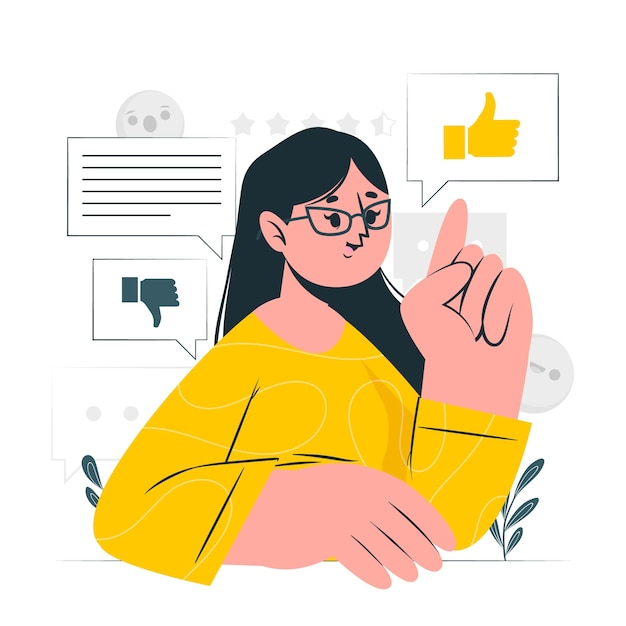
\includegraphics[width=3.70764in,height=3.70764in]{media/image25.jpeg}

\textbf{Fato ou opinião?}

\textbf{Fato} é algo que ocorreu e pode ser comprovado de algum modo,
por meio de determinado documento, números, vídeo, estudo ou registro.
Observe o exemplo:
\end{quote}

\begin{longtable}[]{@{}l@{}}
\toprule
\begin{minipage}[t]{0.97\columnwidth}\raggedright\strut
\begin{quote}
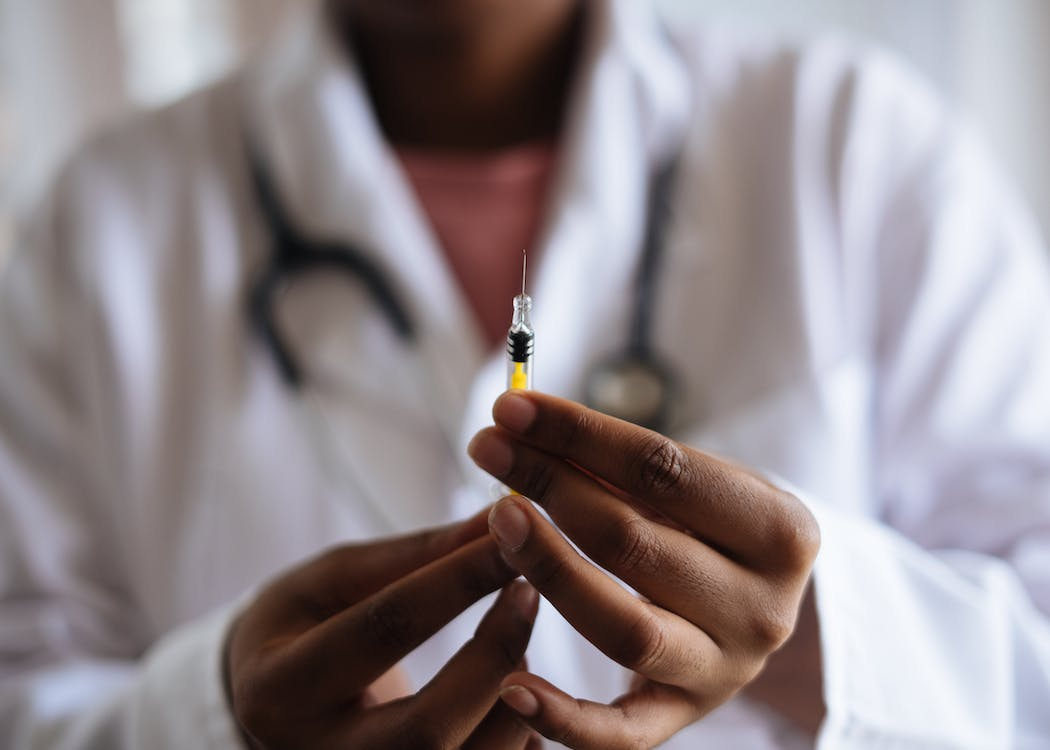
\includegraphics[width=3.07626in,height=2.19722in]{media/image26.jpeg}

https://www.pexels.com/pt-br/foto/pessoa-segurando-injecao-3825529/

Vacinas salvam vidas.
\end{quote}\strut
\end{minipage}\tabularnewline
\bottomrule
\end{longtable}

\begin{quote}
A informação é um fato, tendo em vista que há registros dos casos e, por
meio deles, é possível fazer uma afirmação.

\textbf{Opinião} consiste em uma interpretação do fato, isto é, uma
forma pessoal de olhar o fato. Essa opinião pode ser diferente de pessoa
para pessoa a depender de muitos fatores. Veja o exemplo:
\end{quote}

\begin{longtable}[]{@{}l@{}}
\toprule
\begin{minipage}[t]{0.97\columnwidth}\raggedright\strut
\begin{quote}
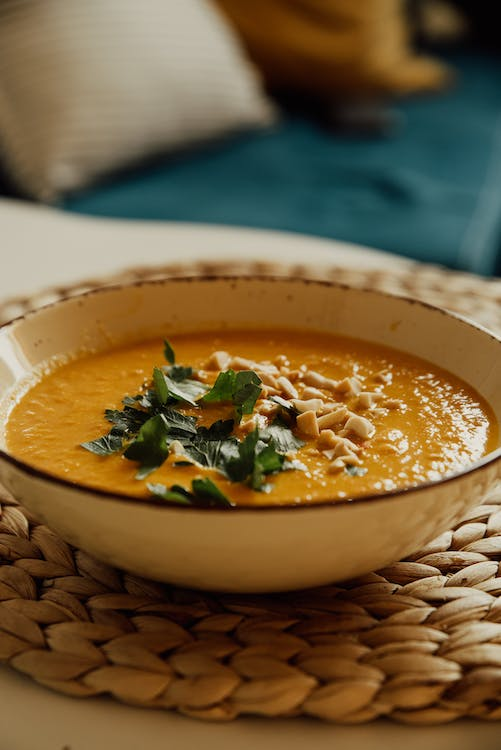
\includegraphics[width=1.98958in,height=2.97842in]{media/image27.jpeg}

https://www.pexels.com/pt-br/foto/prato-de-sopa-em-tigela-de-ceramica-branca-6072108/

Sopa é a melhor comida do mundo!
\end{quote}\strut
\end{minipage}\tabularnewline
\bottomrule
\end{longtable}

\colorsec{Atividades}

\num{1}

\begin{quote}
Leia o texto a seguir.

Realize a primeira leitura, em voz alta, até o fim do texto. Depois da
sua leitura, solicite aos alunos que leiam alternadamente o texto.
Incentive-os a consultar o dicionário quando não entenderem o
significado de alguma palavra.

\textbf{Dia Internacional dos Direitos Humanos}

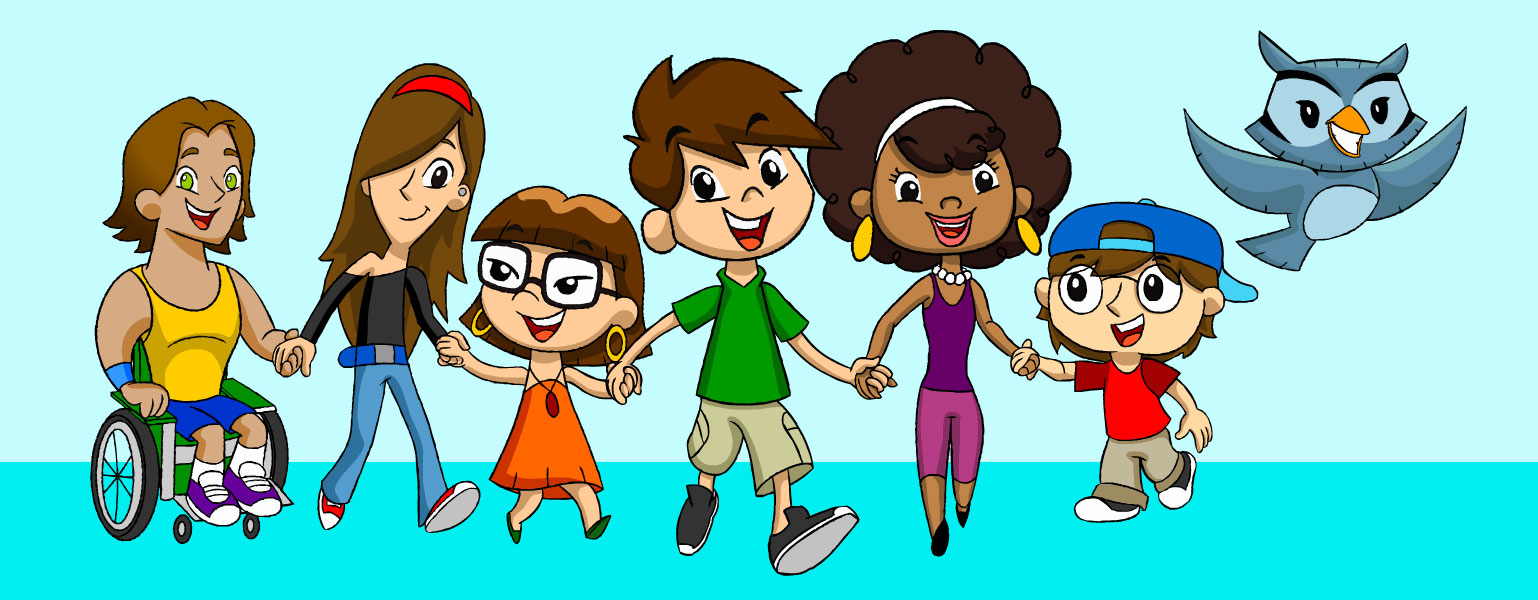
\includegraphics[width=5.90556in,height=3.33125in]{media/image28.jpeg}

18/01/2017~

``Todos os seres humanos nascem livres e iguais em dignidade e
direitos.'' ``São dotados de razão e consciência e devem agir em relação
uns aos outros com espírito de fraternidade''. Esse é o Artigo I de um
documento muito importante chamado Declaração Universal dos Direitos
Humanos.

O texto é um dos documentos básicos da Organização das Nações Unidas que
faz aniversário dia 10 de dezembro, dia em que a Declaração foi
assinada. Na declaração, são enumerados os direitos que todos os seres
humanos têm, sem distinção alguma, seja de raça, de cor, de sexo, de
língua, de religião, de opinião política ou outra, de origem nacional ou
social, de fortuna, de nascimento ou de qualquer outra situação. E, é
claro, devem ser respeitados por todos.

São direitos básicos para promover a liberdade, a justiça e a paz no
mundo (saúde, educação, cultura e arte, liberdade de informação e
expressão, habitação e alimentação adequadas, entre outros). A
declaração serve como um tipo de guia para que governos, entidades e
cidadãos em cada país respeitem e sejam respeitados, além de inspirar
tratados internacionais sobre direitos humanos.

Talvez você não saiba, mas o francês René Cassin, conhecido como ``o
homem dos direitos humanos'', foi um dos ``pais espirituais'' e redator
principal do primeiro projeto de Declaração Universal dos Direitos
Humanos. Ele perseguiu sem descanso a sua missão internacional de
humanista. Assim, por sua ação em favor do ``respeito aos direitos
humanos no contexto mundial'', recebeu, em 1968, o Prêmio Nobel da Paz.

O Dia Internacional dos Direitos Humanos é mais que uma data
comemorativa. É um momento para que todos lembrem e reflitam sobre a
garantia dos direitos humanos na sua comunidade, cidade, país e em todo
o mundo. O respeito a esses direitos e a garantia de uma vida digna
depende da vigilância e participação de todos os povos e nações.

\textbf{Reconhecimento aos defensores dos Direitos Humanos no Brasil\\
}\\
O respeito aos direitos humanos é condição para o desenvolvimento de
qualquer país. Por isso, aqui no Brasil, institui-se o Prêmio Direitos
Humanos. ~Ele é a mais alta condecoração do~governo~brasileiro a pessoas
e entidades que se destacam na defesa e na promoção e também no
enfrentamento e no combate a violações dos direitos humanos no país.

DIA Internacional dos Direitos Humanos. Plenarinho. Disponível em:
https://plenarinho.leg.br/index.php/2017/01/dia-internacional-dos-direitos-humanos/.
Acesso em: 13 mar. 2023.
\end{quote}

\begin{enumerate}
\def\labelenumi{\alph{enumi})}
\item
  Sobre o que trata o texto? Trata sobre o Dia Internacional dos
  Direitos Humanos.
\end{enumerate}

\begin{quote}
\_\_\_\_\_\_\_\_\_\_\_\_\_\_\_\_\_\_\_\_\_\_\_\_\_\_\_\_\_\_\_\_\_\_\_\_\_\_\_\_\_\_\_\_\_\_\_\_\_\_\_\_\_\_\_\_\_\_\_\_\_\_\_\_

\_\_\_\_\_\_\_\_\_\_\_\_\_\_\_\_\_\_\_\_\_\_\_\_\_\_\_\_\_\_\_\_\_\_\_\_\_\_\_\_\_\_\_\_\_\_\_\_\_\_\_\_\_\_\_\_\_\_\_\_\_\_\_\_

\_\_\_\_\_\_\_\_\_\_\_\_\_\_\_\_\_\_\_\_\_\_\_\_\_\_\_\_\_\_\_\_\_\_\_\_\_\_\_\_\_\_\_\_\_\_\_\_\_\_\_\_\_\_\_\_\_\_\_\_\_\_\_\_

b) Qual é o Artigo I da Declaração Universal dos Direitos Humanos?
``Todos os seres humanos nascem livres e iguais em dignidade e
direitos.'' ``São dotados de razão e consciência e devem agir em relação
uns aos outros com espírito de fraternidade''.
\_\_\_\_\_\_\_\_\_\_\_\_\_\_\_\_\_\_\_\_\_\_\_\_\_\_\_\_\_\_\_\_\_\_\_\_\_\_\_\_\_\_\_\_\_\_\_\_\_\_\_\_\_\_\_\_\_\_\_\_\_\_\_\_

\_\_\_\_\_\_\_\_\_\_\_\_\_\_\_\_\_\_\_\_\_\_\_\_\_\_\_\_\_\_\_\_\_\_\_\_\_\_\_\_\_\_\_\_\_\_\_\_\_\_\_\_\_\_\_\_\_\_\_\_\_\_\_\_

\_\_\_\_\_\_\_\_\_\_\_\_\_\_\_\_\_\_\_\_\_\_\_\_\_\_\_\_\_\_\_\_\_\_\_\_\_\_\_\_\_\_\_\_\_\_\_\_\_\_\_\_\_\_\_\_\_\_\_\_\_\_\_\_

\_\_\_\_\_\_\_\_\_\_\_\_\_\_\_\_\_\_\_\_\_\_\_\_\_\_\_\_\_\_\_\_\_\_\_\_\_\_\_\_\_\_\_\_\_\_\_\_\_\_\_\_\_\_\_\_\_\_\_\_\_\_\_\_

c) Por que René Cassin recebeu, em 1968, o Prêmio Nobel da Paz? Por sua
ação em favor do ``respeito aos direitos humanos no contexto mundial''.
\_\_\_\_\_\_\_\_\_\_\_\_\_\_\_\_\_\_\_\_\_\_\_\_\_\_\_\_\_\_\_\_\_\_\_\_\_\_\_\_\_\_\_\_\_\_\_\_\_\_\_\_\_\_\_\_\_\_\_\_\_\_\_\_

\_\_\_\_\_\_\_\_\_\_\_\_\_\_\_\_\_\_\_\_\_\_\_\_\_\_\_\_\_\_\_\_\_\_\_\_\_\_\_\_\_\_\_\_\_\_\_\_\_\_\_\_\_\_\_\_\_\_\_\_\_\_\_\_

\_\_\_\_\_\_\_\_\_\_\_\_\_\_\_\_\_\_\_\_\_\_\_\_\_\_\_\_\_\_\_\_\_\_\_\_\_\_\_\_\_\_\_\_\_\_\_\_\_\_\_\_\_\_\_\_\_\_\_\_\_\_\_\_

\_\_\_\_\_\_\_\_\_\_\_\_\_\_\_\_\_\_\_\_\_\_\_\_\_\_\_\_\_\_\_\_\_\_\_\_\_\_\_\_\_\_\_\_\_\_\_\_\_\_\_\_\_\_\_\_\_\_\_\_\_\_\_\_

d) Segundo o texto, o que é o Prêmio Direitos Humanos? Ele é a mais alta
condecoração do~governo~brasileiro a pessoas e entidades que se destacam
na defesa e na promoção e também no enfrentamento e no combate a
violações dos direitos humanos no país.

\_\_\_\_\_\_\_\_\_\_\_\_\_\_\_\_\_\_\_\_\_\_\_\_\_\_\_\_\_\_\_\_\_\_\_\_\_\_\_\_\_\_\_\_\_\_\_\_\_\_\_\_\_\_\_\_\_\_\_\_\_\_\_\_

\_\_\_\_\_\_\_\_\_\_\_\_\_\_\_\_\_\_\_\_\_\_\_\_\_\_\_\_\_\_\_\_\_\_\_\_\_\_\_\_\_\_\_\_\_\_\_\_\_\_\_\_\_\_\_\_\_\_\_\_\_\_\_\_

\protect\hypertarget{_Hlk128040463}{}{}\_\_\_\_\_\_\_\_\_\_\_\_\_\_\_\_\_\_\_\_\_\_\_\_\_\_\_\_\_\_\_\_\_\_\_\_\_\_\_\_\_\_\_\_\_\_\_\_\_\_\_\_\_\_\_\_\_\_\_\_\_\_\_\_

\_\_\_\_\_\_\_\_\_\_\_\_\_\_\_\_\_\_\_\_\_\_\_\_\_\_\_\_\_\_\_\_\_\_\_\_\_\_\_\_\_\_\_\_\_\_\_\_\_\_\_\_\_\_\_\_\_\_\_\_\_\_\_\_

\_\_\_\_\_\_\_\_\_\_\_\_\_\_\_\_\_\_\_\_\_\_\_\_\_\_\_\_\_\_\_\_\_\_\_\_\_\_\_\_\_\_\_\_\_\_\_\_\_\_\_\_\_\_\_\_\_\_\_\_\_\_\_\_
\end{quote}

\num{2}

\begin{quote}
Nos trechos reproduzidos a seguir, identifique com \textbf{F} o que é
fato ou com \textbf{O} para o que é opinião. Antes da realização desta
atividade, importante salientar aos alunos que um modo de perceber se
alguma informação é um fato ou opinião é observar se ela pode ser
comprovada com evidências (no caso do fato) ou se é possível concordar
ou não com o que é dito (no caso da opinião).

( F ) ``Todos os seres humanos nascem livres e iguais em dignidade e
direitos.'' ``São dotados de razão e consciência e devem agir em relação
uns aos outros com espírito de fraternidade''

( O ) ... ``E, é claro, devem ser respeitados por todos.''

( O ) ... ``A declaração serve como um tipo de guia para que governos,
entidades e cidadãos em cada país respeitem e sejam respeitados, além de
inspirar tratados internacionais sobre direitos humanos''.

( O ) ... ``Talvez você não saiba, mas o francês René Cassin, conhecido
como ``o homem dos direitos humanos''.

( F ) ... ``o francês René Cassin, conhecido como ``o homem dos direitos
humanos'', foi um dos ``pais espirituais'' e redator principal do
primeiro projeto de Declaração Universal dos Direitos Humanos''.
\end{quote}

\num{3}

\begin{quote}
Leia o trecho do texto que fala sobre o Dia Mundial da Liberdade de
Pensamento:

\textbf{Dia Mundial da Liberdade de Pensamento}

Pode ser a~falta~de proximidade, de contato olho no olho; pode ser a
certeza de que não haverá um revide imediato; ou, ainda, a ilusão do
anonimato que a internet proporciona -- o fato é que as pessoas insultam
outras pela web de um jeito que jamais fariam se estivessem frente a
frente. E as redes sociais são o grande palco dessas agressões.

Em todo o mundo, grandes empresas como Facebook, YouTube e Twitter
abriram canais em que os usuários podem denunciar conteúdos e contas que
disseminam ou incentivam a violência. Embora qualquer tipo de agressão
seja passível de punição, há uma que se distingue pela gravidade: é o
discurso de ódio.

O discurso de ódio tem como principal característica o fato de querer
atingir uma~minoria {[}...{]} Ele é especialmente nocivo porque promove
a intolerância e impede a pluralidade de vozes, ferindo assim
a~democracia.

{[}...{]}

Precisamos formar cidadãos que, cada vez mais, saibam que discurso de
ódio não é piada, opinião, polêmica ou controvérsia. Liberdade de
expressão é um direito valiosíssimo, que deve ser usado para fortalecer
a~democracia, não para silenciar minorias.

DIA Mundial da Liberdade de Pensamento. Plenarinho. Disponível em:
https://plenarinho.leg.br/index.php/2021/07/dia-mundial-da-liberdade-de-pensamento/.
Acesso em: 13 mar. 2023.

a) Escreva um trecho do texto que expressa:

Ajude os estudantes a diferenciar fato de opinião, pois esse tema é um
tanto complexo para eles, mas é\\
fundamental que, de modo gradual, eles se\\
habituem a realizar esse tipo de análise.
\end{quote}

\begin{itemize}
\item
  o \textbf{fato} que foi noticiado: Foi noticiado sobre o Dia Mundial
  da Liberdade de Pensamento e o combate ao discurso de ódio.
\end{itemize}

\begin{quote}
\_\_\_\_\_\_\_\_\_\_\_\_\_\_\_\_\_\_\_\_\_\_\_\_\_\_\_\_\_\_\_\_\_\_\_\_\_\_\_\_\_\_\_\_\_\_\_\_\_\_\_\_\_\_\_\_\_\_\_\_\_\_\_\_

\_\_\_\_\_\_\_\_\_\_\_\_\_\_\_\_\_\_\_\_\_\_\_\_\_\_\_\_\_\_\_\_\_\_\_\_\_\_\_\_\_\_\_\_\_\_\_\_\_\_\_\_\_\_\_\_\_\_\_\_\_\_\_\_

\_\_\_\_\_\_\_\_\_\_\_\_\_\_\_\_\_\_\_\_\_\_\_\_\_\_\_\_\_\_\_\_\_\_\_\_\_\_\_\_\_\_\_\_\_\_\_\_\_\_\_\_\_\_\_\_\_\_\_\_\_\_\_\_
\end{quote}

\begin{itemize}
\item
  \begin{quote}
  A \textbf{opinião} dos autores do texto: Sugestão de resposta:
  Precisamos formar cidadãos que, cada vez mais, saibam que discurso de
  ódio não é piada, opinião, polêmica ou controvérsia.
  \end{quote}
\end{itemize}

\begin{quote}
\_\_\_\_\_\_\_\_\_\_\_\_\_\_\_\_\_\_\_\_\_\_\_\_\_\_\_\_\_\_\_\_\_\_\_\_\_\_\_\_\_\_\_\_\_\_\_\_\_\_\_\_\_\_\_\_\_\_\_\_\_\_\_\_

\_\_\_\_\_\_\_\_\_\_\_\_\_\_\_\_\_\_\_\_\_\_\_\_\_\_\_\_\_\_\_\_\_\_\_\_\_\_\_\_\_\_\_\_\_\_\_\_\_\_\_\_\_\_\_\_\_\_\_\_\_\_\_\_

\_\_\_\_\_\_\_\_\_\_\_\_\_\_\_\_\_\_\_\_\_\_\_\_\_\_\_\_\_\_\_\_\_\_\_\_\_\_\_\_\_\_\_\_\_\_\_\_\_\_\_\_\_\_\_\_\_\_\_\_\_\_\_\_
\end{quote}

\begin{itemize}
\item
  \begin{quote}
  O \textbf{motivo} da opinião dos autores do texto: Liberdade de
  expressão é um direito valiosíssimo, que deve ser usado para
  fortalecer a~democracia, não para silenciar minorias.
  \end{quote}
\end{itemize}

\begin{quote}
\_\_\_\_\_\_\_\_\_\_\_\_\_\_\_\_\_\_\_\_\_\_\_\_\_\_\_\_\_\_\_\_\_\_\_\_\_\_\_\_\_\_\_\_\_\_\_\_\_\_\_\_\_\_\_\_\_\_\_\_\_\_\_\_

\_\_\_\_\_\_\_\_\_\_\_\_\_\_\_\_\_\_\_\_\_\_\_\_\_\_\_\_\_\_\_\_\_\_\_\_\_\_\_\_\_\_\_\_\_\_\_\_\_\_\_\_\_\_\_\_\_\_\_\_\_\_\_\_

\_\_\_\_\_\_\_\_\_\_\_\_\_\_\_\_\_\_\_\_\_\_\_\_\_\_\_\_\_\_\_\_\_\_\_\_\_\_\_\_\_\_\_\_\_\_\_\_\_\_\_\_\_\_\_\_\_\_\_\_\_\_\_\_
\end{quote}

\colorsec{Treino}

\num{1}

\begin{quote}
(Fácil) Leia o trecho de uma carta do leitor.

\textbf{Fogo na Amazônia}

É um absurdo a ineficácia das autoridades responsáveis por esse assunto
{[}\ldots{}{]}. Parecem ignorar que na região o Exército tem Batalhões
de Selva, a Marinha tem embarcações preparadas e batalhões de fuzileiros
navais, e a Força Aérea, aeronaves de patrulhamento para agir de
imediato assim que se detecta o início de um desmatamento ou de um foco
de incêndio.

Com tudo isso, poderiam impedir essas situações e prender os envolvidos.
Mas o resultado aí está, com o fogo atingindo o Pantanal e a fumaça já
chegando até o Rio Grande do Sul.

PAINEL DO LEITOR. Disponível em:
https://www1.folha.uol.com.br/paineldoleitor/2020/09/fome-assim-no-brasil-no-seculo-21-e-barbarie-diz-leitor.shtml.
Acesso em: 15 mar. 2023.

Com base na leitura da carta do leitor, pode-se identificar que o leitor
quis apresentar

(A) uma sugestão para o jornal realizar uma reportagem a respeito do
tema.

(B) uma opinião sobre uma questão publicada no jornal.

(C) uma crítica ao veículo jornalístico sobre a questão da Amazônia.

(D) um questionamento às autoridades sobre a questão da Amazônia.

Saeb D13 - Estabelecer, no interior de um texto, relação entre um fato e
uma opinião relativa a este fato.

BNCC: EF04LP15: Distinguir fatos de opiniões/sugestões em textos
(informativos, jornalísticos, publicitários etc.).

(A) Incorreta. O texto não traz uma sugestão para o jornal, mas a
opinião do autor da carta.

(B) Correta. No trecho ``É um absurdo a ineficácia das autoridades
responsáveis por esse assunto'', pode-se identificar o objetivo da carta
do leitor de expressar sua opinião sobre o assunto publicado no jornal.

(C) Incorreta. A crítica é direcionada ao governo.

(D) Incorreta. Não foi realizado nenhum questionamento.
\end{quote}

\num{2}

\begin{quote}
(Médio) Leia um trecho da reportagem a seguir.

\textbf{População brasileira é a 5ª mais feliz do mundo, diz pesquisa}

Os brasileiros nunca foram tão felizes, mas apenas quatro em cada dez
estão satisfeitos com a economia, segundo uma pesquisa do instituto
Ipsos que avaliou a felicidade da população em 32 países.

No Brasil, 83\% dos entrevistados consideram-se muito felizes ou felizes
--- uma alta de 20 pontos percentuais em relação ao último levantamento,
feito em dezembro de 2021, quando o índice foi de 63\%. No mundo, a
percepção de felicidade também subiu, de 67\% para 73\%.

"As pessoas estão vendo este ano como o encerramento de um capítulo
extremamente desafiador em nossa história: a covid-19, ainda que a
pandemia não tenha sido totalmente erradicada, seu impacto é
infinitamente menor do que nos últimos anos. Esse sentimento reforça a
percepção de felicidade", diz Marcos Calliari, CEO da Ipsos no Brasil.

POPULAÇÃO brasileira é a 5ª mais feliz do mundo, diz pesquisa. BBC
Brasil. Disponível em:
https://www.bbc.com/portuguese/articles/cye4ll78l3wo. Acesso em: 16 mar.
2023.

\protect\hypertarget{_Hlk128058360}{}{}No terceiro parágrafo, o trecho
que está entre aspas mostra a

(A) opinião do autor da reportagem.

(B) opinião do CEO da Ipsos no Brasil.

(C) explicação sobre a pesquisa.

(D) opinião dos entrevistados.

Saeb D13 - Estabelecer, no interior de um texto, relação entre um fato e
uma opinião relativa a este fato.

BNCC: EF04LP15: Distinguir fatos de opiniões/sugestões em textos
(informativos, jornalísticos, publicitários etc.).

.

(A) Incorreta. Não existe, na reportagem, a opinião do autor da
reportagem.

(B) Correta. As aspas indicam a opinião do CEO da Ipsos no Brasil.

(C) Incorreta. O especialista não explica os resultados da pesquisa no
trecho entre aspas.

(D) Incorreta. Inexiste a opinião dos entrevistados no trecho em
questão.
\end{quote}

\num{3}

\begin{quote}
(Difícil) Leia o texto a seguir.

\protect\hypertarget{_Hlk129854304}{}{}\textbf{'Corvo-Correio', da
escritora Isabel Cintra, também foi lançado em Angola}

José é um corvo que sonhava voar para entregar cartinhas ao lado dos
pombos brancos. No entanto, o irredutível chefe do serviço postal do
bosque, Coruja Mafalda, não permite. "Mas você é um corvo! Certamente já
deve ter ouvido dizer que os corvos não servem para carteiros. Todos
sabem disso!", diz. Após ser praticamente ignorado e rejeitado, José
decide ir embora da região. Mas o jogo vira quando o inverno chega. O
livro infantil Corvo-Correio fala sobre valores como tolerância,
igualdade e representatividade, conceitos que precisam ser cada vez mais
trabalhados com os pequeninos\protect\hypertarget{_Hlk129854481}{}{}.
~"O Corvo José é orgulhosamente meu pássaro negro mensageiro. Na
verdade, este protagonista cheio de força sempre esteve presente em
algum lugar em mim, durante toda a minha infância e se escondia
assustado a cada situação de preconceito vivida. Foi preciso uma espera
de crescimento, abandonar o silêncio da criança para deixar a coragem
emergir em forma de palavras que propagam afeto", explica a autora
Isabel Cintra.~

'CORVO-CORREIO', da escritora Isabel Cintra, também foi lançado em
Angola. Estadão. Disponível em:
https://www.estadao.com.br/emais/comportamento/livro-infantil-traz-licoes-sobre-preconceito-exclusao-e-resiliencia/.
Acesso em: 16 mar. 2023.

Um trecho que apresenta um fato sobre o conteúdo do livro é

(A) "O Corvo José é orgulhosamente meu pássaro negro mensageiro''.

(B) \protect\hypertarget{_Hlk129854629}{}{}``{[}...{]} fala sobre
valores como tolerância, igualdade e representatividade, conceitos que
precisam ser cada vez mais trabalhados com os pequeninos''.

(C) ``Na verdade, este protagonista cheio de força sempre esteve
presente em algum lugar em mim''...

(D) ``Foi preciso uma espera de crescimento, abandonar o silêncio da
criança para deixar a coragem emergir em forma de palavras que propagam
afeto''.

Saeb D13 - Estabelecer, no interior de um texto, relação entre um fato e
uma opinião relativa a este fato.

BNCC: EF04LP15: Distinguir fatos de opiniões/sugestões em textos
(informativos, jornalísticos, publicitários etc.).

(A) Incorreta. Nesse trecho é expressa a visão da autora sobre o livro.

(B) Correta. Em ``{[}...{]} fala sobre valores como tolerância,
igualdade e representatividade, conceitos que precisam ser cada vez mais
trabalhados com os pequeninos'''', há apresentação de um fato.

(C) Incorreta. O trecho aborda a identificação da autora com o
personagem.

(D) Incorreta. O trecho mostra como a autora produziu a obra.
\end{quote}

\chapter{Infográficos}
\markboth{Módulo 9}{}

\begin{quote}
Neste módulo, os alunos vão interpretar infográficos, relacionando-os
aos contextos nos quais estão inseridos.
\end{quote}

\subsection{Conteúdo}\label{conteuxfado-8}

\begin{quote}
\textbf{Infográficos}

https://www.pexels.com/pt-br/foto/realizacao-conquista-facanha-sucesso-7948039/

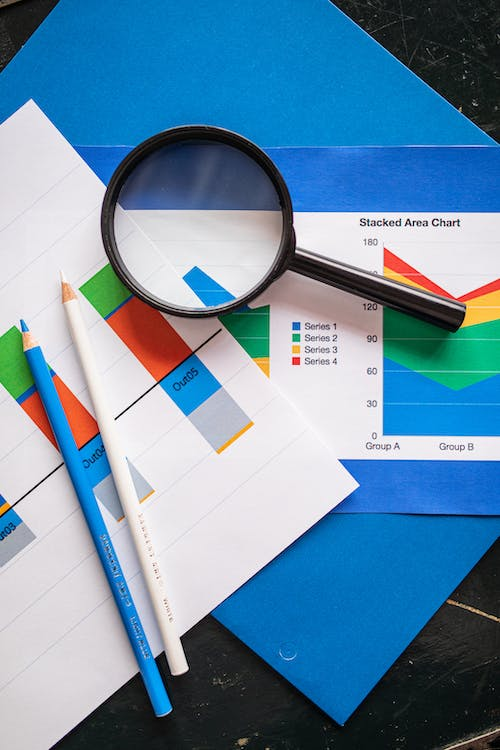
\includegraphics[width=2.81075in,height=4.21050in]{media/image29.jpeg}

Infográficos servem para informar ou explicar algo de modo breve,
objetivo, dinâmico e em linguagem acessível por meio de textos curtos
escritos e elementos não verbais. Os temas abordados nos infográficos
costumam tratar das mais diversificadas áreas.

Normalmente, os infográficos podem ser encontrados em revistas, jornais
e \emph{sites} da internet, acompanhando, complementando e/ou resumindo
as informações veiculadas em notícias, reportagens, entrevistas, textos
informativos etc. Há também infográficos que apresentam as informações
``sozinhos'', isto é, sem fazer parte de um texto jornalístico.

Nos infográficos, as informações podem ser apresentadas por meio de
desenhos, fotos, gráficos, tabelas, mapas, cores, formas, entre outros
recursos visuais, e de textos curtos e dados numéricos. Pode apresentar
título, imagens e legendas em sua composição.

Os infográficos são exemplos da multimodalidade, isto é, apresentam
várias linguagens (escrita, visual, verbal) em um mesmo texto.
\end{quote}

\colorsec{Atividades}

\begin{quote}
Explicar aos alunos que este gráfico é conhecido como gráfico de barras.
Caso julgue pertinente, mostre aos alunos como se elabora um gráfico
usando um programa de computador.
\end{quote}

\num{1}

\begin{quote}
Leia um trecho da notícia a seguir e analise os infográficos, observando
suas funções e as informações apresentadas.

\textbf{Recicla Santos quase dobra coleta de recicláveis no último
semestre - confira infográfico}

PUBLICADO:~31~DE~JANEIRO~DE~2018~

18h~20

Coordenador de Políticas Ambientais da Secretaria de Meio Ambiente,
Marcus Fernandes atribui os resultados diretamente ao Recicla Santos.
``Entre junho e julho de 2017, a coleta seletiva passou de 270 para 420
toneladas. Nos 26 anos de história, nunca houve um aumento nessa
dimensão''.

Fernandes lembra que a aplicação do Recicla Santos foi precedida de
palestras, encontros e reuniões realizadas pela Prefeitura para divulgar
a lei entre a população.

Além de aliviar o aterro sanitário do Sítio das Neves, o aumento da
reciclagem traz efeitos positivos para a sociedade e todo o planeta.
``Temos de lembrar, por exemplo, que para se fabricar plástico se gasta
petróleo. A reciclagem reduz a retirada de matéria prima para a produção
de diversos tipos de produtos. Estamos, assim, utilizando menos água e
energia elétrica''.

O coordenador lembra, ainda, que a nova lei criou postos de trabalho na
área da reciclagem. Atualmente, há duas cooperativas de catadores
atuando na Cidade, a Comares e a Sem Fronteira.

{[}...{]}

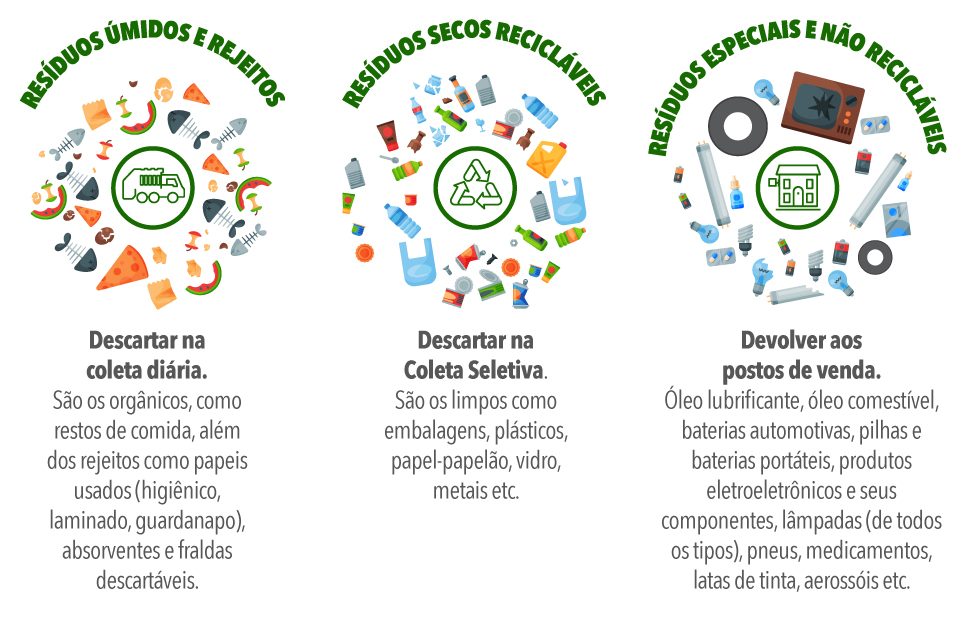
\includegraphics[width=5.90556in,height=3.90764in]{media/image30.jpeg}

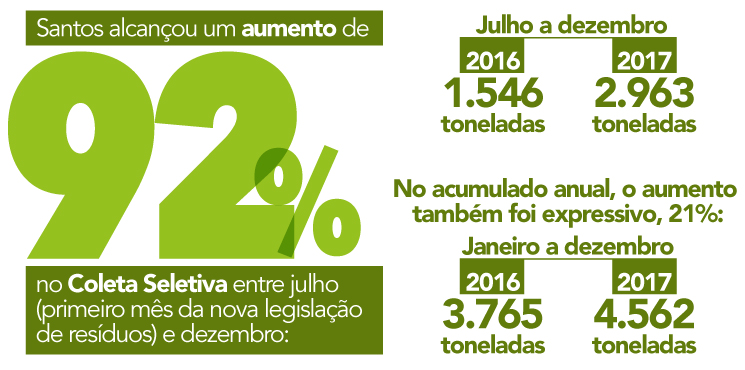
\includegraphics[width=5.90556in,height=2.92847in]{media/image31.jpeg}

PREFEITURA de Santos. Recicla Santos quase dobra coleta de recicláveis
no último semestre - confira infográfico. Disponível em:
\textless{}https://www.santos.sp.gov.br/?q=noticia/recicla-santos-quase-dobra-coleta-de-reciclaveis-no-ultimo-semestre-confira-infografico\textgreater{}.
Acesso em: 17 mar. 2023.

a) Qual é a finalidade desses infográficos? A finalidade dos
infográficos é acrescentar novas informações, demonstrar com a linguagem
não verbal o que está sendo exposto no texto verbal.

\_\_\_\_\_\_\_\_\_\_\_\_\_\_\_\_\_\_\_\_\_\_\_\_\_\_\_\_\_\_\_\_\_\_\_\_\_\_\_\_\_\_\_\_\_\_\_\_\_\_\_\_\_\_\_\_\_\_\_\_\_\_\_\_

\_\_\_\_\_\_\_\_\_\_\_\_\_\_\_\_\_\_\_\_\_\_\_\_\_\_\_\_\_\_\_\_\_\_\_\_\_\_\_\_\_\_\_\_\_\_\_\_\_\_\_\_\_\_\_\_\_\_\_\_\_\_\_\_

\_\_\_\_\_\_\_\_\_\_\_\_\_\_\_\_\_\_\_\_\_\_\_\_\_\_\_\_\_\_\_\_\_\_\_\_\_\_\_\_\_\_\_\_\_\_\_\_\_\_\_\_\_\_\_\_\_\_\_\_\_\_\_\_
\end{quote}

\begin{enumerate}
\def\labelenumi{\alph{enumi})}
\item
  Por que recursos como esse são importantes em textos informativos?
  Porque possibilitam maior compreensão do assunto e, dessa forma,
  facilitam a leitura e a compreensão.
\end{enumerate}

\begin{quote}
\_\_\_\_\_\_\_\_\_\_\_\_\_\_\_\_\_\_\_\_\_\_\_\_\_\_\_\_\_\_\_\_\_\_\_\_\_\_\_\_\_\_\_\_\_\_\_\_\_\_\_\_\_\_\_\_\_\_\_\_\_\_\_\_

\_\_\_\_\_\_\_\_\_\_\_\_\_\_\_\_\_\_\_\_\_\_\_\_\_\_\_\_\_\_\_\_\_\_\_\_\_\_\_\_\_\_\_\_\_\_\_\_\_\_\_\_\_\_\_\_\_\_\_\_\_\_\_\_

\_\_\_\_\_\_\_\_\_\_\_\_\_\_\_\_\_\_\_\_\_\_\_\_\_\_\_\_\_\_\_\_\_\_\_\_\_\_\_\_\_\_\_\_\_\_\_\_\_\_\_\_\_\_\_\_\_\_\_\_\_\_\_\_

\_\_\_\_\_\_\_\_\_\_\_\_\_\_\_\_\_\_\_\_\_\_\_\_\_\_\_\_\_\_\_\_\_\_\_\_\_\_\_\_\_\_\_\_\_\_\_\_\_\_\_\_\_\_\_\_\_\_\_\_\_\_\_\_

c) De acordo com o segundo infográfico, qual foi o aumento no Coleta
Seletiva entre julho e dezembro? Foi de 92\%.

\_\_\_\_\_\_\_\_\_\_\_\_\_\_\_\_\_\_\_\_\_\_\_\_\_\_\_\_\_\_\_\_\_\_\_\_\_\_\_\_\_\_\_\_\_\_\_\_\_\_\_\_\_\_\_\_\_\_\_\_\_\_\_\_

\_\_\_\_\_\_\_\_\_\_\_\_\_\_\_\_\_\_\_\_\_\_\_\_\_\_\_\_\_\_\_\_\_\_\_\_\_\_\_\_\_\_\_\_\_\_\_\_\_\_\_\_\_\_\_\_\_\_\_\_\_\_\_\_

d) Qual foi o aumento no acumulado anual? 21\%.

\_\_\_\_\_\_\_\_\_\_\_\_\_\_\_\_\_\_\_\_\_\_\_\_\_\_\_\_\_\_\_\_\_\_\_\_\_\_\_\_\_\_\_\_\_\_\_\_\_\_\_\_\_\_\_\_\_\_\_\_\_\_\_\_

\_\_\_\_\_\_\_\_\_\_\_\_\_\_\_\_\_\_\_\_\_\_\_\_\_\_\_\_\_\_\_\_\_\_\_\_\_\_\_\_\_\_\_\_\_\_\_\_\_\_\_\_\_\_\_\_\_\_\_\_\_\_\_\_

e) Marque CD para o que deve descartado na coleta diária, CS para o que
deve ser descartado na coleta seletiva e D para o que deve ser devolvido
aos postos de venda.

( CS ) Resíduos limpos.

( CD ) Resíduos orgânicos.

( D ) Resíduos especiais.

f) Há quantas cooperativas atuando na cidade de Santos? Quais são elas?
Há duas cooperativas, a Comares e a Sem Fronteira.

\_\_\_\_\_\_\_\_\_\_\_\_\_\_\_\_\_\_\_\_\_\_\_\_\_\_\_\_\_\_\_\_\_\_\_\_\_\_\_\_\_\_\_\_\_\_\_\_\_\_\_\_\_\_\_\_\_\_\_\_\_\_\_\_

\_\_\_\_\_\_\_\_\_\_\_\_\_\_\_\_\_\_\_\_\_\_\_\_\_\_\_\_\_\_\_\_\_\_\_\_\_\_\_\_\_\_\_\_\_\_\_\_\_\_\_\_\_\_\_\_\_\_\_\_\_\_\_\_

\_\_\_\_\_\_\_\_\_\_\_\_\_\_\_\_\_\_\_\_\_\_\_\_\_\_\_\_\_\_\_\_\_\_\_\_\_\_\_\_\_\_\_\_\_\_\_\_\_\_\_\_\_\_\_\_\_\_\_\_\_\_\_\_

g) Um recurso bastante utilizado em infográficos é a variedade de
tamanhos e cores das letras. Em sua opinião, fazer essa diferença visual
no texto verbal do infográfico é importante? Por quê? Resposta pessoal.
Espera-se que os alunos respondam que esses recursos são utilizados para
colocar em destaque certos elementos que o produtor do infográfico
deseja que o leitor visualize e também para organizar as informações.

\_\_\_\_\_\_\_\_\_\_\_\_\_\_\_\_\_\_\_\_\_\_\_\_\_\_\_\_\_\_\_\_\_\_\_\_\_\_\_\_\_\_\_\_\_\_\_\_\_\_\_\_\_\_\_\_\_\_\_\_\_\_\_\_

\_\_\_\_\_\_\_\_\_\_\_\_\_\_\_\_\_\_\_\_\_\_\_\_\_\_\_\_\_\_\_\_\_\_\_\_\_\_\_\_\_\_\_\_\_\_\_\_\_\_\_\_\_\_\_\_\_\_\_\_\_\_\_\_

\_\_\_\_\_\_\_\_\_\_\_\_\_\_\_\_\_\_\_\_\_\_\_\_\_\_\_\_\_\_\_\_\_\_\_\_\_\_\_\_\_\_\_\_\_\_\_\_\_\_\_\_\_\_\_\_\_\_\_\_\_\_\_\_
\end{quote}

\colorsec{Treino}

\num{1}

(Fácil) Leia o infográfico a seguir que traz informações relacionadas a
como fazer um clube de leitura.

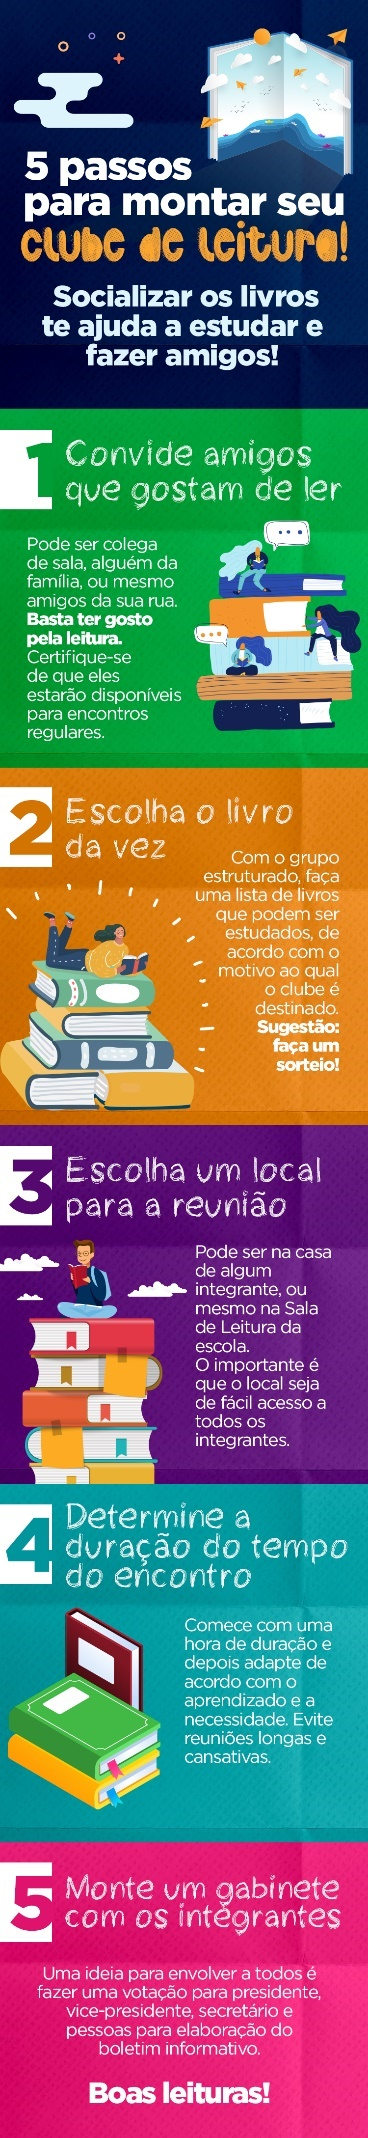
\includegraphics[width=1.67569in,height=9.72500in]{media/image32.jpeg}

SECRETARIA da Educação do Estado de São Paulo. Infográfico: saiba como
montar um clube de leitura. Disponível em:
\textless{}www.educacao.sp.gov.br/noticia/infografico-saiba-como-montar-um-clube-de-leitura/\textgreater{}.
Acesso em: 17 mar. 2023.

Uma das características principais do infográfico é apresentar

(A) informações do dia a dia.

(B) texto de ficção.

(C) assuntos relacionados ao ato de ler.

(D) texto verbal e texto não verbal.

Saeb D4 - Identificar o tema central do texto.

BNCC: EF04LP20: Reconhecer a função de gráficos, diagramas e tabelas em
textos, como forma de apresentação de dados e informações.

(A) Incorreta. Essa não é a característica fundamental do gênero.

(B) Incorreta. O infográfico apresenta texto informativo.

(C) Incorreta. Infográficos podem apresentar qualquer tipo de tema.

(D) Correta. A característica principal do gênero infográfico é
apresentar imagens e textos.

\num{2}

(Médio) O infográfico mostra a presença de alunos estrangeiros na rede
estadual de ensino no Estado de São Paulo.

\begin{quote}
https://www.educacao.sp.gov.br/infografico-alunos-estrangeiros-na-rede-estadual-de-ensino/

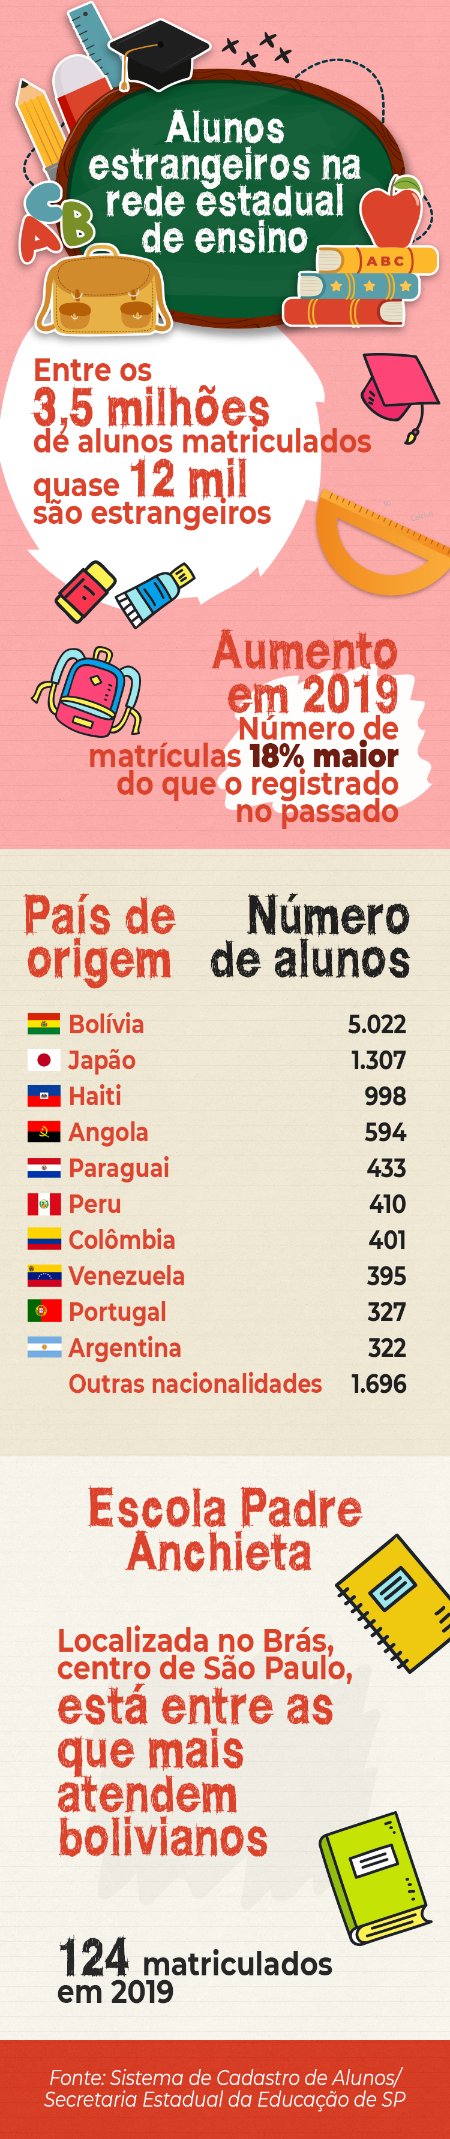
\includegraphics[width=2.04375in,height=9.72500in]{media/image33.png}
\end{quote}

SECRETARIA da Educação do Estado de São Paulo. \#Infográfico: alunos
estrangeiros na rede estadual de ensino.

Disponível em:
\textless{}www.educacao.sp.gov.br/noticias/infografico-alunos-estrangeiros-na-rede-estadual-de-ensino/\textgreater{}.
Acesso em: 18 mar. 2023.

Podemos observar no infográfico que o número de matrículas em 2019 foi

(A) 3,5 vezes maior do que o registrado no ano anterior.

(B) 18\% maior do que o registrado no ano anterior.

(C) 124\% maior do que o registrado no ano anterior.

(D) 12 mil vezes maior que o registrado no ano anterior.

Saeb D3 - Estabelecer relação entre informações num texto ou entre
diferentes textos.

BNCC: EF04LP20: Reconhecer a função de gráficos, diagramas e tabelas em
textos, como forma de apresentação de dados e informações.

(A) Incorreta. O número 3,5 está presente em: ``entre os 3,5 milhões de
alunos matriculados, quase 12 mil são estrangeiros''.

(B) Correta. Conforme informações do infográfico, o número de matrículas
em 2019 foi 18\% maior que o registrado no ano anterior.

(C) Incorreta. O número 124 refere-se ao número de alunos matriculados
em 2019, mas não é o dado que apresenta o aumento em relação ao ano
anterior.

(D) Incorreta. O número 12 mil aparece em: ``entre os 3,5 milhões de
alunos matriculados, quase 12 mil são estrangeiros''.

\num{3}

(Difícil) Leia o infográfico a seguir.

www.inca.gov.br/en/node/3201

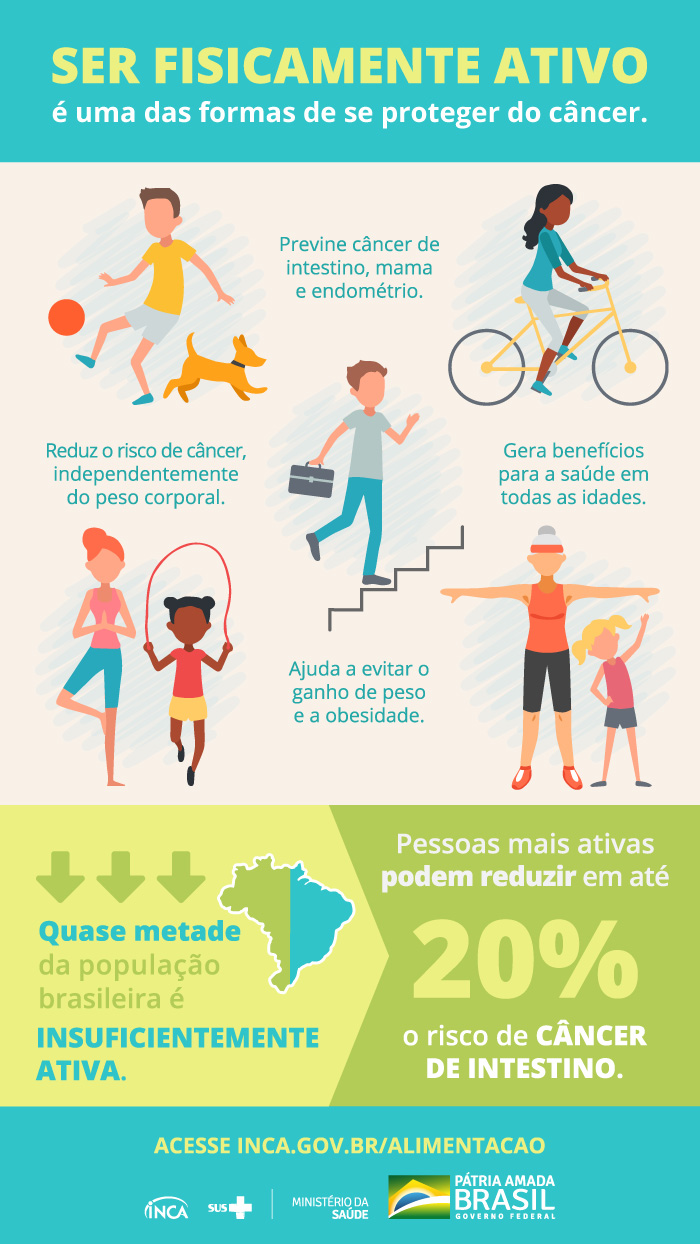
\includegraphics[width=3.58333in,height=6.36458in]{media/image34.jpeg}

\protect\hypertarget{_Hlk40547643}{}{}

ATIVIDADE física para o controle do câncer. Disponível em:
\textless{}www.inca.gov.br/en/node/3201\textgreater{}. Acesso em: 18
mar. 2023.

Qual é o tema central do infográfico?

(A) a quantidade de brasileiros que praticam esportes.

(B) a atividade física e a prevenção do câncer.

(C) os malefícios de ser uma pessoa insuficientemente ativa.

(D) os tipos de atividades físicas que previnem o câncer.

Saeb D4 - Identificar o tema central do texto.

BNCC: EF04LP20: Reconhecer a função de gráficos, diagramas e tabelas em
textos, como forma de apresentação de dados e informações.

(A) Incorreta. O infográfico não mostra as atividades que previnem o
câncer.

(B) Correta. O infográfico mostra que fazer atividade física previne o
câncer.

(C) Incorreta. Apenas foi mencionada a quantidade de brasileiros
insuficientemente ativos.

(D) Incorreta. O infográfico não mostra os tipos que previnem o câncer.

\chapter{Coesão textual}
\markboth{Módulo 10}{}

\begin{quote}
Nesta seção, os alunos vão analisar palavras utilizadas em trechos de
texto para fazer referência aos substantivos; verificar o sentido
expresso por essas palavras e observar que estabelecem ligação entre os
trecho; identificar os pronomes anafóricos e estabelecer a coesão ao
completar trechos com eles.
\end{quote}

\subsection{Conteúdo}\label{conteuxfado-9}

\begin{quote}
https://www.istockphoto.com/br/foto/bal\%C3\%A3o-de-di\%C3\%A1logo-letras-em-cortar-revista-gm518358614-89988479?phrase=palavras

\textbf{Coesão }

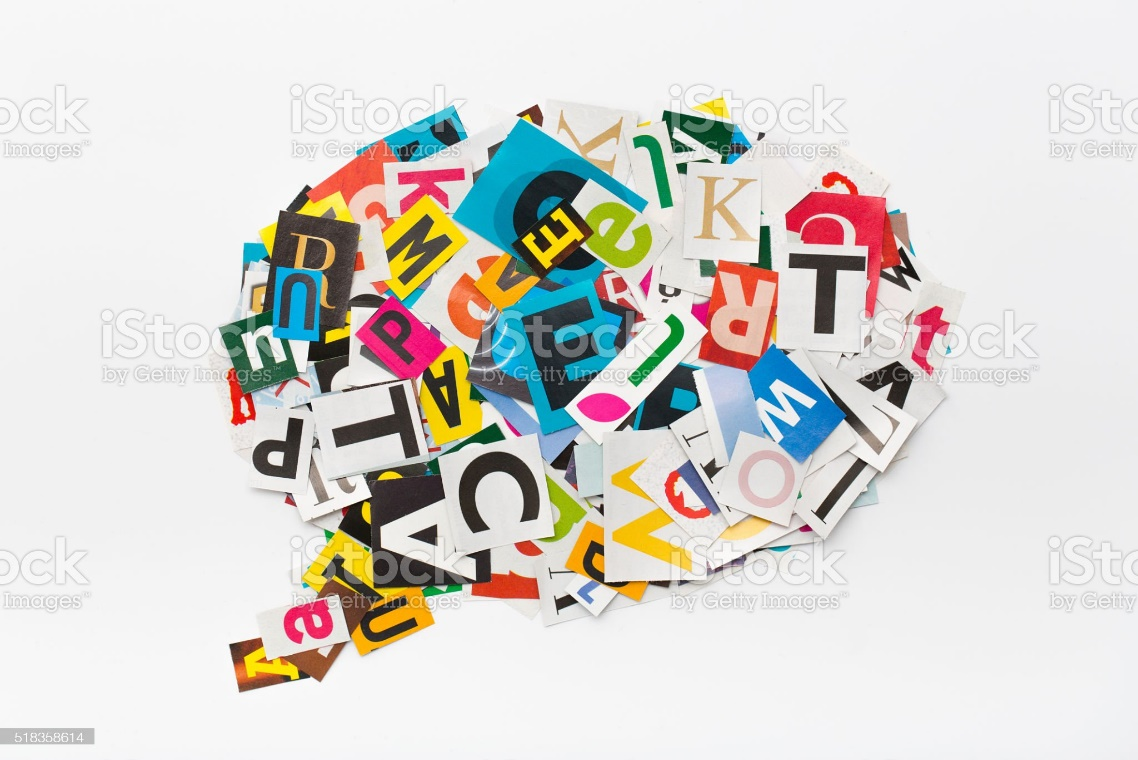
\includegraphics[width=5.17173in,height=3.44883in]{media/image35.jpeg}

Na língua portuguesa, há palavras e expressões que podem ser usadas para
ligar as ideias e relacionar os parágrafos, dando progressão ao texto.

\textbf{Coesão} consiste na ligação entre os elementos gramaticais.
Refere-se ao modo como as frases e palavras se relacionam e são
combinadas. A coerência, por sua vez, é a formação lógica do texto, o
que dá sentido por meio de uma linguagem e sequência adequadas. Sem
coesão, o texto fica sem qualquer conexão entre as partes. E sem
coerência, ele confunde o leitor. Um texto coeso e coerente assegura que
a sua produção textual cumpra a sua finalidade: comunicar algo,
convencer o leitor ou impactar de algum modo.

Por meio da coesão referencial, cria-se um sistema de relações entre as
palavras e expressões dentro de um texto, fazendo com que o leitor
reconheça os termos aos quais se referem. O termo que indica a entidade
ou situação a que o falante se refere é chamado de referente.

Coesão por referência: há palavras cuja função é fazer referência, como
os pronomes e os sinônimos:

Pronomes pessoais: eu, tu, ele, nós, vós, eles..., pronomes possessivos:
meu, teu, seu, nosso..., pronomes demonstrativos: este, esse, aquele...,
pronomes indefinidos: algum, nenhum, todo..., pronomes relativos: que, o
qual, onde...
\end{quote}

\colorsec{Atividades}

\num{1}

\begin{quote}
Leia a narrativa a seguir. Sugere-se propor inicialmente uma leitura
silenciosa. Após a leitura, retomar os aspectos que chamaram a atenção
de cada aluno. Pode-se fazer, em seguida, uma leitura compartilhada,
parágrafo a parágrafo, conversando sobre as palavras desconhecidas e as
impressões relacionadas ao texto.

https://www.istockphoto.com/br/vetor/ugly-duckling-bullying-concept-vector-cartoon-ilustra\%C3\%A7\%C3\%A3o-gm1372690734-441739165?utm\_source=pixabay\&utm\_medium=affiliate\&utm\_campaign=SRP\_illustration\_sponsored\&utm\_content=https\%3A\%2F\%2Fpixabay.com\%2Fpt\%2Fillustrations\%2Fsearch\%2Fpatinho\%2520feio\%2F\&utm\_term=patinho+feio

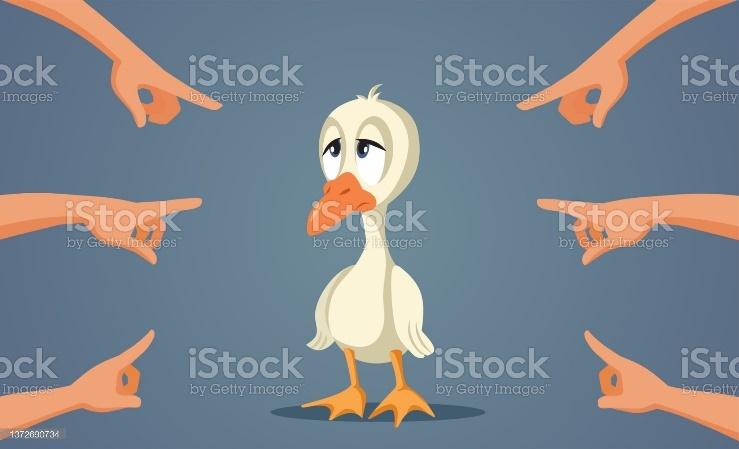
\includegraphics[width=3.35140in,height=2.03748in]{media/image36.jpeg}
\end{quote}

\textbf{O patinho feio}

Em uma bonita manhã de outono, a pata Sofia construiu seu ninho de
gravetos perto do lago. Então passou a chocar. E, depois de trinta e
três dias, cinco de seis ovos se quebraram, e os filhotinhos nasceram
--- todos belos e saudáveis.

Sorrindo, a bicharada foi visitar a mamãe e os bebês:

--- Que lindos patinhos, tão amarelinhos, já aprendendo a nadar. Sejam
bem-vindos!

Mas ainda havia um ovo, que não se abria.

--- Será que não vingará? --- os animais se perguntavam.

Preocupada e esperançosa, Sofia continuou a chocar. Enfim a casca
trincou, e nasceu uma avezinha bem diferente, que não tinha a mesma cor
e graciosidade de seus irmãos. A família achava isso estranho:

--- Quá-quá-quá!

--- Aquele patinho é cinzento!

--- Patinho desajeitado!

--- Patinho feio!

O pobrezinho era sempre excluído, sentindo-se triste e solitário. De
tanto sofrer, resolveu fugir.

Nadou durante todo o dia, em busca de um lar que o acolhesse. Já
anoitecendo, o patinho chegou a uma lagoa cheia de marrecos. Ele se
aproximou e tentou se agrupar. Novamente zombaram dele:

--- Você não pertence à nossa família, pato feio, que não sabe
mergulhar!

Rejeitado, o patinho partiu. Não só nadou, como andou muito. Quando
quase se abeirava de um rio, viu um bando de gansos flutuando sobre as
águas.

--- Eles são cinzas e se parecem comigo. Achei a minha família!

Mas os gansos o expulsaram com ruídos estridentes:

--- Não aceitamos estranhos em nosso lar!

No entanto, o patinho desprezado nunca desistia... Enquanto procurava,
ia crescendo e se emplumando. Certo dia, encontrou uma grande lagoa,
onde viviam aves de pescoços longos e sinuosos, de plumas alvas, com
elegância inigualável.

Essas aves foram dóceis com o recém-chegado. Então, ele resolveu ficar
todo o inverno, sendo bem cuidado e amado.

No início da primavera, em uma manhã perfumada pelas cerejeiras, o pato
acordou com um grande alvoroço:

--- Que linda plumagem! Quanta beleza!

Sem acreditar nos elogios, ele olhou para o reflexo na água e se deu
conta de que pertencia àquela família. Na verdade, o patinho feio era um
cisne - o mais bonito de todos!

\textbf{ANDERSEN, Hans Christian.} O patinho feio. Disponível em:
https://alfabetizacao.mec.gov.br/images/conta-pra-mim/livros/versao\_digital/o\_patinho\_feio\_versao\_digital.pdf.
Acesso em: 18 mar. 2023.

a) Sobre o que trata o texto? Sobre um patinho que acreditava ser feio
até descobrir que era um belo cisne.
\_\_\_\_\_\_\_\_\_\_\_\_\_\_\_\_\_\_\_\_\_\_\_\_\_\_\_\_\_\_\_\_\_\_\_\_\_\_\_\_\_\_\_\_\_\_\_\_\_\_\_\_\_\_\_\_\_\_\_\_\_\_\_\_

\_\_\_\_\_\_\_\_\_\_\_\_\_\_\_\_\_\_\_\_\_\_\_\_\_\_\_\_\_\_\_\_\_\_\_\_\_\_\_\_\_\_\_\_\_\_\_\_\_\_\_\_\_\_\_\_\_\_\_\_\_\_\_\_

\_\_\_\_\_\_\_\_\_\_\_\_\_\_\_\_\_\_\_\_\_\_\_\_\_\_\_\_\_\_\_\_\_\_\_\_\_\_\_\_\_\_\_\_\_\_\_\_\_\_\_\_\_\_\_\_\_\_\_\_\_\_\_\_

b) Qual era a cor do último patinho a nascer? Cinzento.

\_\_\_\_\_\_\_\_\_\_\_\_\_\_\_\_\_\_\_\_\_\_\_\_\_\_\_\_\_\_\_\_\_\_\_\_\_\_\_\_\_\_\_\_\_\_\_\_\_\_\_\_\_\_\_\_\_\_\_\_\_\_\_\_

c) O fim da história relata uma descoberta do patinho. Que descoberta
foi essa? O patinho feio descobriu que era um lindo cisne.

\_\_\_\_\_\_\_\_\_\_\_\_\_\_\_\_\_\_\_\_\_\_\_\_\_\_\_\_\_\_\_\_\_\_\_\_\_\_\_\_\_\_\_\_\_\_\_\_\_\_\_\_\_\_\_\_\_\_\_\_\_\_\_\_

\protect\hypertarget{_Hlk130128820}{}{}\_\_\_\_\_\_\_\_\_\_\_\_\_\_\_\_\_\_\_\_\_\_\_\_\_\_\_\_\_\_\_\_\_\_\_\_\_\_\_\_\_\_\_\_\_\_\_\_\_\_\_\_\_\_\_\_\_\_\_\_\_\_\_\_

\_\_\_\_\_\_\_\_\_\_\_\_\_\_\_\_\_\_\_\_\_\_\_\_\_\_\_\_\_\_\_\_\_\_\_\_\_\_\_\_\_\_\_\_\_\_\_\_\_\_\_\_\_\_\_\_\_\_\_\_\_\_\_\_

\num{2}

Releia o trecho a seguir:

\begin{longtable}[]{@{}l@{}}
\toprule
\begin{minipage}[t]{0.97\columnwidth}\raggedright\strut
~ ~

Nadou durante todo o dia, em busca de um lar que o acolhesse. Já
anoitecendo, o patinho chegou a uma lagoa cheia de marrecos. \emph{Ele}
se aproximou e tentou se agrupar.\strut
\end{minipage}\tabularnewline
\bottomrule
\end{longtable}

a) Sublinhe a palavra usada para fazer referência ao patinho feio.

b) Por que essa palavra foi usada? Para substituir o nome patinho, de
modo a evitar a repetição.

\_\_\_\_\_\_\_\_\_\_\_\_\_\_\_\_\_\_\_\_\_\_\_\_\_\_\_\_\_\_\_\_\_\_\_\_\_\_\_\_\_\_\_\_\_\_\_\_\_\_\_\_\_\_\_\_\_\_\_\_\_\_\_\_

\_\_\_\_\_\_\_\_\_\_\_\_\_\_\_\_\_\_\_\_\_\_\_\_\_\_\_\_\_\_\_\_\_\_\_\_\_\_\_\_\_\_\_\_\_\_\_\_\_\_\_\_\_\_\_\_\_\_\_\_\_\_\_\_

\begin{longtable}[]{@{}l@{}}
\toprule
Nadou durante todo o dia, em busca de um lar que o
acolhesse\tabularnewline
\bottomrule
\end{longtable}

\num{3}

A palavra \textbf{o} aparece duas vezes nesta frase, com funções
diferentes.

a) Qual dessas palavras tem a função de determinar o substantivo
\textbf{dia}? O primeiro \textbf{o}.

\_\_\_\_\_\_\_\_\_\_\_\_\_\_\_\_\_\_\_\_\_\_\_\_\_\_\_\_\_\_\_\_\_\_\_\_\_\_\_\_\_\_\_\_\_\_\_\_\_\_\_\_\_\_\_\_\_\_\_\_\_\_\_\_

\_\_\_\_\_\_\_\_\_\_\_\_\_\_\_\_\_\_\_\_\_\_\_\_\_\_\_\_\_\_\_\_\_\_\_\_\_\_\_\_\_\_\_\_\_\_\_\_\_\_\_\_\_\_\_\_\_\_\_\_\_\_\_\_

b) Qual delas foi usada para substituir a palavra patinho? O segundo
\textbf{o}.

\_\_\_\_\_\_\_\_\_\_\_\_\_\_\_\_\_\_\_\_\_\_\_\_\_\_\_\_\_\_\_\_\_\_\_\_\_\_\_\_\_\_\_\_\_\_\_\_\_\_\_\_\_\_\_\_\_\_\_\_\_\_\_\_

\_\_\_\_\_\_\_\_\_\_\_\_\_\_\_\_\_\_\_\_\_\_\_\_\_\_\_\_\_\_\_\_\_\_\_\_\_\_\_\_\_\_\_\_\_\_\_\_\_\_\_\_\_\_\_\_\_\_\_\_\_\_\_\_

\num{4}

Quando existe muita repetição em um texto, ele fica com pouca qualidade.
Leia o texto a seguir e observe.

\begin{longtable}[]{@{}l@{}}
\toprule
O \textbf{Patinho Feio}, na verdade, transformou-se em um cisne
belíssimo. O \textbf{Patinho Feio} ficou muito feliz com essa nova
condição. Os amigos do \textbf{Patinho Feio} fizeram uma grande festa
para homenagear o \textbf{Patinho Feio}. \textbf{O Patinho Feio e seus
amigos} se divertiram muito!\tabularnewline
\bottomrule
\end{longtable}

a) Reescreva o trecho e elimine as repetições que não são necessárias,
mantendo a clareza do texto. Sugestão de resposta: O Patinho Feio, na
verdade, transformou-se em um cisne belíssimo. Ele ficou muito feliz com
essa nova condição. Os amigos dele fizeram uma grande festa para
homenageá-lo. Eles se divertiram muito!

\_\_\_\_\_\_\_\_\_\_\_\_\_\_\_\_\_\_\_\_\_\_\_\_\_\_\_\_\_\_\_\_\_\_\_\_\_\_\_\_\_\_\_\_\_\_\_\_\_\_\_\_\_\_\_\_\_\_\_\_\_\_\_\_

\_\_\_\_\_\_\_\_\_\_\_\_\_\_\_\_\_\_\_\_\_\_\_\_\_\_\_\_\_\_\_\_\_\_\_\_\_\_\_\_\_\_\_\_\_\_\_\_\_\_\_\_\_\_\_\_\_\_\_\_\_\_\_\_

\_\_\_\_\_\_\_\_\_\_\_\_\_\_\_\_\_\_\_\_\_\_\_\_\_\_\_\_\_\_\_\_\_\_\_\_\_\_\_\_\_\_\_\_\_\_\_\_\_\_\_\_\_\_\_\_\_\_\_\_\_\_\_\_

\_\_\_\_\_\_\_\_\_\_\_\_\_\_\_\_\_\_\_\_\_\_\_\_\_\_\_\_\_\_\_\_\_\_\_\_\_\_\_\_\_\_\_\_\_\_\_\_\_\_\_\_\_\_\_\_\_\_\_\_\_\_\_\_

\_\_\_\_\_\_\_\_\_\_\_\_\_\_\_\_\_\_\_\_\_\_\_\_\_\_\_\_\_\_\_\_\_\_\_\_\_\_\_\_\_\_\_\_\_\_\_\_\_\_\_\_\_\_\_\_\_\_\_\_\_\_\_\_

\_\_\_\_\_\_\_\_\_\_\_\_\_\_\_\_\_\_\_\_\_\_\_\_\_\_\_\_\_\_\_\_\_\_\_\_\_\_\_\_\_\_\_\_\_\_\_\_\_\_\_\_\_\_\_\_\_\_\_\_\_\_\_\_

b) Que alterações no texto você fez evitar as repetições? Foram usados
pronomes.

\_\_\_\_\_\_\_\_\_\_\_\_\_\_\_\_\_\_\_\_\_\_\_\_\_\_\_\_\_\_\_\_\_\_\_\_\_\_\_\_\_\_\_\_\_\_\_\_\_\_\_\_\_\_\_\_\_\_\_\_\_\_\_\_

\_\_\_\_\_\_\_\_\_\_\_\_\_\_\_\_\_\_\_\_\_\_\_\_\_\_\_\_\_\_\_\_\_\_\_\_\_\_\_\_\_\_\_\_\_\_\_\_\_\_\_\_\_\_\_\_\_\_\_\_\_\_\_\_

\num{5}

Leia o trecho a seguir e responda: Que pronome pode ser usado no trecho
a seguir para evitar a repetição?

\begin{longtable}[]{@{}l@{}}
\toprule
Eu, minha mãe e meu irmão assistimos ao filme O Patinho Feio na casa da
minha madrinha. \textbf{Eu, minha mãe e meu irmão} adoramos passar esse
tempo juntos.\tabularnewline
\bottomrule
\end{longtable}

\_\_\_\_\_\_\_\_\_\_Nós\_\_\_\_\_\_\_\_\_\_\_\_\_\_\_\_\_\_\_\_\_\_\_\_\_\_\_\_\_\_\_\_\_\_\_\_\_\_\_\_\_\_\_\_\_\_\_\_\_\_\_\_\_\_

\colorsec{Treino}

\num{1}

(Fácil) Leia a charadinha a seguir.

\begin{longtable}[]{@{}l@{}}
\toprule
\begin{minipage}[t]{0.97\columnwidth}\raggedright\strut
\begin{quote}
Você sabe por que a água foi presa?

Porque ela matou a sede.
\end{quote}\strut
\end{minipage}\tabularnewline
\bottomrule
\end{longtable}

\begin{quote}
A palavra ``ela'' se refere a

(A) ``presa''.

(B) ``sede''.

(C) ``água''.

(D) ``matou''.

Saeb D2 - Inferir uma afirmação implícita num texto.

BNCC Não há correspondência.

(A) Incorreta. A palavra ``ela'' não pode retomar ``presa''.

(B) Incorreta. A palavra ``ela'' não pode retomar ``sede''.

(C) Correta. O pronome ``ela'' está substituindo a palavra ``água'',

(D) Incorreta. Pronomes retomam substantivos, e não verbos.
\end{quote}

\num{2}

\begin{quote}
(Médio) Leia o trecho de uma carta do leitor sobre uma reportagem
publicada na Revista Planeta.

A reportagem ``Voluntários sem fronteira'' (edição nº 470) me emocionou
do início ao fim devido à riqueza de detalhes e imagens de Moçambique.
Tenho 16 anos e pretendo ser médica. Agora, mais do que nunca, sei que é
essa a profissão que quero para minha vida, {[}...{]} seguir exemplos de
pessoas como os médicos citados na reportagem. Esses profissionais
sacrificam sua vida para ajudar ao próximo e não buscam reconhecimento
ou algo parecido, e sim a valorização da vida de cidadãos que não
possuem ninguém por eles, mas, mesmo assim, ``transmitem a alegria de
viver''. {[}...{]}

REVISTA PLANETA. Cartas. Disponível em:
www.revistaplaneta.com.br/cartas-29/. Acesso em: 18 mar. 2023.

No trecho ``não possuem ninguém por eles'', a palavra ``eles'' se refere
aos

(A) ``médicos''.

(B) ``cidadãos''.

(C) ``profissionais''.

(D) ``detalhes''.''.

Saeb D9 - Realizar inferências e antecipações em relação ao conteúdo e à
intencionalidade a partir de indicadores como tipo de texto e
características gráficas.

BNCC: Não há correspondência.

(A) Incorreta. O pronome ``eles'' não retoma os ``médicos''.

(B) Correta. O pronome ``eles'' retoma os ``cidadãos que não possuem
ninguém''.

(C) Incorreta. O pronome não retoma os ``profissionais''.

(D) Incorreta. O pronome não se refere aos ``detalhes''.
\end{quote}

\num{3}

\begin{quote}
(Difícil) Leia a piadinha a seguir.

- Uma criança vai pela rua com seu avô e encontra um caramelo no chão.
Vai pegá-lo, e seu avô lhe diz: 'não se pega nada do chão'.

Mais adiante a criança encontra uma moeda de um~real e seu avô lhe diz:
'não se pega nada do chão'.~

Seguem caminhando e seu avô tropeça e cai no chão, e pede ajuda à
criança. E ela lhe diz: 'vovô, não se pega nada do chão'.

Disponível em:
https://br.guiainfantil.com/piadas-infantis/144-piadas-de-crianca-para-crianca.html.
Acesso em: 18 mar. 2023.

No trecho ``Vai pegá-lo, e seu avô lhe diz: 'não se pega nada do
chão'.'', ``-lo'' está sendo usado no lugar da palavra

(A) ``criança''.

(B) ``chão''.

(C) ``caramelo''.

(D) ``avô''.

Saeb D2 - Inferir uma afirmação implícita num texto.

BNCC Não há correspondência.

(A) Incorreta. O pronome não está retomando ``criança''.

(B) Incorreta. O pronome não está retomando ``chão''.

(C) Correta. ``lo'' está substituindo ``caramelo''.

(D) Incorreta. O pronome não pode retomar um substantivo.
\end{quote}

\chapter{Simulado 1}
\markboth{Simulado 1}{}

\num{1}

\begin{quote}
Leia o trecho da notícia.

\textbf{Lei proíbe casamento a menores de 16 anos}

Você sabia que o Brasil, em números absolutos, é o quarto país onde mais
ocorrem casamentos infantis? E que 36\% das mulheres daqui se casam
antes de completarem os 18 anos? Isso é o que aponta uma pesquisa do
Banco Mundial, divulgada em 2015. Mas a perspectiva é que essa realidade
mude. Isso porque, em março de 2019, foi aprovada a Lei 13.811/19, que
proíbe o casamento para menores de 16 anos. Isso significa que agora, de
acordo com o texto, ``não será permitido, em qualquer caso, o casamento
de quem não atingiu a idade núbil'', no caso, 16 anos.

PLENARINHO. Lei proíbe casamento a menores de 16 anos. Disponível em:

\url{https://plenarinho.leg.br/index.php/2019/03/lei-proibe-casamento-menores-de-16-anos}.
Acesso em: 19 mar. 2023.

As características que dão credibilidade ao texto informativo são

(A) números e dados apresentados com base em pesquisas de confiança e
referências do local em que a pesquisa foi publicada.

(B) opiniões pessoais, números e dados apresentados com base em
pesquisas de opinião realizadas com leitores.

(C) citações de especialistas, números e dados apresentados com base em
pesquisas de confiança, além de linguagem clara e subjetiva.

(D) linguagem clara e objetiva, opiniões pessoais, números e dados
apresentados com base em pesquisas de confiança.

Saeb D1 - Localizar informações num texto.

BNCC EF35LP03: Identificar a ideia central do texto, demonstrando
compreensão global.

(A) Correta. No trecho, frases como ``36\% das mulheres daqui se casam
antes de completarem os 18 anos {[}...{]} aponta uma pesquisa do Banco
Mundial, divulgada em 2015'' apresentam números e dados com base em
pesquisas de confiança e referências do local em que a pesquisa foi
publicada, características que conferem credibilidade ao texto
informativo.

(B) Incorreta. Opiniões pessoais e pesquisas de opinião realizadas com
leitores não dão credibilidade ao texto informativo, sendo ausentes no
trecho em questão.

(C) Incorreta. Linguagem subjetiva não confere credibilidade ao texto
informativo e está ausente no trecho, e o texto não apresenta citações
de especialistas.

(D) Incorreta. Opiniões pessoais não dão credibilidade ao texto
informativo e inexistem no trecho citado.
\end{quote}

\num{2}

A reportagem ``Seres humanos cresceram 8,6 centímetros nos últimos cem
anos'' apresenta os resultados de um mapeamento sobre altura.

\textbf{Seres humanos cresceram 8,6 centímetros nos últimos cem anos}

Segundo uma pesquisa realizada pela revista E-Life, os homens mais altos
do mundo são os holandeses (com uma média de 1,83m) e as mulheres da
Letônia (1,70). Os mais baixinhos são do Timor Leste (1,60m) e as
mulheres da Guatemala (1,50m). O estudo mapeou a tendência de
crescimento em quase 200 países desde 1914.

Os pesquisadores afirmam que as mudanças nos padrões de crescimento
aconteceram,

principalmente, por influências climáticas. Porém, a genética e as
condições de saúde,

saneamento e nutrição também têm sua contribuição nestas alterações.

BRASILEIROS cresceram 8,6 centímetros nos últimos cem anos. Disponível
em:

www.ebc.com.br/infantil/voce-sabia/2016/07/brasileiros-cresceram-86-centimetros-nos-ultimos-

cem-anos. Acesso em: 19 mar. 2023.

Segundo a reportagem, a média de altura dos homens do Timor Leste é

\begin{quote}
(A) menor que a das mulheres da Letônia.

(B) menor que a das mulheres da Guatemala.

(C) maior que a dos homens da Holanda.

(D) igual a das mulheres da Letônia.

Saeb D2 - Inferir uma afirmação implícita num texto.

BNCC EF35LP04 - Inferir informações implícitas nos textos lidos.

(A) Correta. A média de altura dos homens do Timor Leste (1,60 m) é
menor que a média de altura das mulheres da Letônia (1,7 0m).

(B) Incorreta. A média de altura das mulheres da Guatemala é 1,50 m, e a
dos homens do Timor Leste é 1,60 m.

(C) Incorreta. A média de altura dos homens da Holanda é 1,83m, e a dos
homens do Timor Leste é 1,60m.

(D) Incorreta. A média de altura das mulheres da Letônia é 1,70 m, e a
dos homens do Timor Leste é 1,60 m.
\end{quote}

\num{3}

\begin{quote}
Leia um trecho do poema ``O ramo verde'', de Adelina.

O ramo verde

{[}\ldots{}{]}

Foram à tarde a passeio

no jardim os dois; Sofia

colhia rosas; em meio

disse ao irmão: --- que alegria!

Vou dar à mamãe um \textbf{ramo}

das minhas amadas flores! {[}\ldots{}{]}

VIEIRA, Adelina Lopes. O ramo verde. Disponível em:

\href{http://www.dominiopublico.gov.br/download/texto/wk000077.pdf}{www.dominiopublico.gov.br/download/texto/wk000077.pdf}.
Acesso em: 19 mar. 2023.

A palavra destacada no texto pode ser substituída, sem perda de sentido,
por:

(A) ramalhete.

(B) arbusto.

(C) grama.

(D) espinho.

Saeb D5 - Inferir o sentido de uma palavra ou expressão a partir do
contexto imediato.

BNCC EF35LP05 - Inferir o sentido de palavras ou expressões
desconhecidas em textos, com base no contexto da frase ou do texto.

(A) Correta. A palavra ``ramo'' pode ser substituída por ``ramalhete'',
que seria um punhado de flores.

(B) Incorreta. Não é possível entender que a palavra ``ramo'' significa
``arbusto'',

(C) Incorreta. Não é possível entender, pela leitura do trecho, que o
significado da palavra ``ramo'' é ``grama''.

(D) Incorreta. Não é possível compreender, pela leitura do trecho, que o
significado da palavra ``ramo'' seja ``espinho'',.
\end{quote}

\num{4}

\begin{quote}
O poema ``Dom Quixote'' mostra os irmãos Paulo e Mário unindo forças
para atingir um objetivo em comum.

\textbf{Dom Quixote}

Paulo tinha seis anos incompletos;

tinha só quatro o louro e gentil Mário.

Foram à biblioteca, sorrateiros,

e ficaram instantes, mudos, quietos,

a espreitar se alguém vinha; então, ligeiros

como o vento, correram para o armário,

que encerrava os volumes cobiçados:

eram dois grandes livros encarnados,

cheios de formosíssimas gravuras,

mas pesados, meu Deus!

Os pequeninos

porfiavam, cansados, vermelhitos,

por tirá-los da estante. Que torturas!

{[}...{]}

vamos ver à vontade o D. Quixote,

sem os ralhos ouvir, impertinentes,

da avó, que adormeceu. Oh! que ventura!

VIEIRA, Adelina Lopes. Dom Quixote. Disponível em:
www.dominiopublico.gov.br/download/texto/wk000074.pdf. Acesso em: 19
mar. 2023.

cobiçados: desejados

porfiavam: competiam

ralhos: censuras

A intenção dos irmãos era

(A) pegar dois livros da estante sem serem vistos.

(B) conseguir entrar na biblioteca sem que a avó os visse.

(C) brincar na biblioteca sem que fossem vistos.

(D) brincar na biblioteca à vontade, sem as interrupções da avó.

Saeb D1 - Localizar informações num texto.

BNCC EF15LP03 - Localizar informações explícitas em textos.

(A) Correta. Os irmãos querem pegar escondidos dois livros da estante da
biblioteca.

(B) Incorreta. Eles já estavam na biblioteca, a intenção era conseguir
pegar os livros.

(C) Incorreta. Eles não queriam brincar.

(D) Incorreta. Os irmãos não queriam brincar.
\end{quote}

\chapter{Simulado 2}
\markboth{Simulado 2}{}

\num{1}

\begin{quote}
Leia a fábula para responder à questão.

\textbf{Os viajantes e o urso}

Dois homens viajavam juntos quando, de repente, surgiu um urso de dentro
da floresta e parou diante deles, urrando. um dos homens tratou de subir
na árvore mais próxima e agarrar-se aos ramos. o outro, vendo que não
tinha tempo para esconder-se, deitou-se no chão, esticado, fingindo de
morto {[}\ldots{}{]}.

\textbf{Na hora do perigo é que se conhece os amigos.}

OS VIAJANTES e o urso. Disponível em:
www.dominiopublico.gov.br/download/texto/me000589.pdf. Acesso em: 19
mar. 2023.

Na leitura da fábula, pode-se compreender que o homem que subiu na
árvore

(A) abandonou o amigo no perigo, em vez de ajudá-lo.

(B) pensou rápido em como ele e seu amigo podiam se proteger.

(C) ajudou seu amigo, pois mostrou uma forma de se esconder.

(D) aconselhou o amigo a se fingir de morto para se esconder.

Saeb D4 - Identificar o tema central do texto.

BNCC EF35LP29: Identificar, em narrativas, cenário, personagem central,
conflito gerador, resolução e o ponto de vista com base no qual
histórias são narradas, diferenciando narrativas em primeira e terceira
pessoas.

(A) Correta. O texto caracteriza o homem que subiu na árvore como um
homem não confiável, já que esse abandonou seu amigo durante uma
situação de perigo.

(B) Incorreta. O homem pensou apenas em si mesmo, já que subiu a árvore
sem ajudar o seu amigo.

(C) Incorreta. O homem não ajudou seu amigo, apenas se escondeu, sem
tentar ajudar o amigo.

(D) Incorreta. O texto não apresenta a informação de que o primeiro
homem avisou o amigo sobre uma das estratégias de se proteger do urso.
\end{quote}

\num{2}

\begin{quote}
Leia o trecho de uma carta do leitor coletiva.

Olá, CHC! Somo alunos do 5º ano. Lemos durante toda a semana na nossa
roda de leitura curiosidades e histórias da revista CHC. Lemos o texto
Por que o cérebro nunca deixa de aprender? e achamos muito legal.
Gostamos da parte que fala que o cérebro de uma criança armazena
informações muito mais rapidamente que o de um adulto. Por isso, vamos
continuar lendo as matérias publicadas na revista. Assim vamos aprender
muito mais, não acha?

Alunos do 5º ano D. Escola Estadual José Ariano Rodrigues. Lins/SP.

Claro que sim!!! Vocês são demais! Escrevam sempre!

CIÊNCIA HOJE DAS CRIANÇAS. Neurônios em movimento. Disponível em:

http://chc.org.br/artigo/fala-aqui/. Acesso em: 19 mar. 2023.

Pela leitura da carta do leitor, entende-se que o seu tema central é

(A) a discussão sobre o texto ``Por que o cérebro nunca deixa de
aprender?'', mostrando o gosto dos alunos por ele.

(B) a pergunta para a revista se eles concordam que ler mais permite que
se aprenda mais também.

(C) a roda de leitura que as crianças fazem na escola para discutir
sobre os textos da revista.

(D) a frequência com que as crianças leem a revista, sendo que, por
isso, elas aprenderão muito mais.

Saeb D4 - Identificar o tema central do texto.

BNCC EF04LP10: Ler e compreender, com autonomia, cartas pessoais de
reclamação, dentre outros gêneros do campo da vida cotidiana, de acordo
com as convenções do gênero carta e considerando a situação comunicativa
e o tema/assunto/finalidade do texto.

(A) Correta. O tema central é a discussão sobre o texto que os alunos
leram na revista ``Por que o cérebro nunca deixa de aprender?''.

(B) Incorreta. Esse é um assunto da carta, e não o seu tema.

(C) Incorreta. Esse não é o tema da carta, pois não é discutida essa
roda, mas sim o texto que eles leram da revista e como eles gostaram
dele.

(D) Incorreta. Essa frequência não é o tema da carta.
\end{quote}

\num{3}

\begin{quote}
Leia um trecho do conto tradicional ``João e Maria'', duas crianças
muito pobres.

\textbf{João e Maria}

Às margens de uma extensa mata existia, há muito tempo, uma cabana
pobre, feita de

troncos de árvore, na qual morava um lenhador com sua segunda esposa e
seus dois

filhinhos, nascidos do primeiro casamento. O garoto chamava-se João e a
menina, Maria.

IRMÃOS GRIMM. ``João e Maria''. Disponível em:

www.dominiopublico.gov.br/download/texto/me000589.pdfAcesso em: 19 mar.
2023.

No trecho, os artigos

(A) ``um'' e ``uma'' são utilizados para se referir a seres que não
estão vivos.

(B) ``o'' e ``a'' são utilizados para se referir às personagens
principais.

(C) femininos são utilizados para se referir a seres que não estão
vivos.

(D) masculinos são utilizados para todas as personagens da história.

Saeb D12-Estabelecer relação entre partes de um texto a partir de
mecanismos de concordância verbal e nominal.

BNCC EF04LP07 - Identificar em textos e usar na produção textual a
concordância entre artigo, substantivo e adjetivo (concordância no grupo
nominal).

(A) Incorreta. O uso de ``um'' para se referir ao lenhador torna essa
alternativa inválida.

(B) Correta. O texto refere-se às personagens principais João e Maria
por artigos definidos ``o'' e ``a'', diferente de ``uma extensa mata'',
``uma cabana pobre'' e ``um

lenhador'', referidos por artigos indefinidos.

(C) Incorreta. A utilização de ``a'' para caracterizar a menina, Maria,
torna essa alternativa inválida

(D) Incorreta. Os artigos masculinos são usados para caracterizarem os
personagens masculinos.

..
\end{quote}

\num{4}

\begin{quote}
Quando não se sabe o significado de uma palavra, muitas vezes, é
possível inferi-lo a partir da análise do contexto em que ela está
inserida.

\textbf{Dos 4 aos 6 anos, crianças têm um salto de desenvolvimento em
autonomia}

Quando completam 4 anos de idade as crianças já percorreram um amplo
caminho de desenvolvimento. Estão já bastante independentes e conseguem
fazer algumas atividades simples da rotina praticamente sem ajuda, como
escovar os dentes, escolher as roupas e se vestir. Nessa etapa, é muito
importante incentivar essas conquistas e apoiar sua crescente autonomia.
{[}...{]}

Ao longo dessa etapa, também haverá muitos ganhos \textbf{cognitivos}. A
capacidade de raciocínio aumenta e possibilita que a criança faça
relações mais complexas. Com 6 anos, muitas já conseguem levar em
consideração regras de diferentes situações sociais e diferenciar com
clareza acontecimentos reais daqueles que são faz-de-conta.

DOS 4 AOS 6 ANOS, crianças têm um salto de desenvolvimento em autonomia.
Disponível em:
www.ebc.com.br/infantil/para-pais/2016/10/dos-4-aos-6-anos-criancas-tem-um-salto-de-desenvolvimento-em-autonomia.
Acesso em: 19 mar. 2023.

Fazendo uma análise da palavra destacada no trecho e com base em seu
contexto em seu significado é relativo

(A) ao ganho de conhecimento.

(B) ao desenvolvimento da fala.

(C) aos movimentos corporais.

(D) às regras de convívio.

Saeb D5 - Inferir o sentido de uma palavra ou expressão a partir do
contexto imediato.

BNCC EF35LP05 - Inferir o sentido de palavras ou expressões
desconhecidas em textos, com base no contexto da frase ou do texto.

(A) Correta. Pela análise do contexto, pode-se inferir que seu
significado é relativo ao ganho de conhecimento.

(B) Incorreta. É relativo ao ganho de conhecimento, e não ao
desenvolvimento da fala.

(C) Incorreta. Não há menção aos movimentos corporais.

(D) Incorreta. Não há menção às regras de convívio.
\end{quote}

\chapter{Simulado 3}
\markboth{Simulado 3}{}

\num{1}

\begin{quote}
As instruções de jogos são textos que apresentam o passo a passo de como
realizar o jogo. Se alterarmos algo, as informações e os objetivos
mudam, assim como a forma de jogar. É preciso ler as regras e descobrir
como se joga e, depois, jogar.

Qual é o elemento fundamental nas instruções de jogos?

(A) Modo de preparar.

(B) Penalizar o perdedor.

(C) Definir um vencedor.

(D) Desenhos das regras definidas.

Saeb D3 - Estabelecer relação entre informações num texto ou entre
diferentes textos.

BNCC EF04LP09: Ler e compreender, com autonomia, boletos, faturas e
carnês, dentre outros gêneros do campo da vida cotidiana, de acordo com
as convenções do gênero (campos, itens elencados, medidas de consumo,
código de barras) e considerando a situação comunicativa e a finalidade
do texto.

(A) Incorreta. Não existe ``modo de preparo'' em instruções de jogos,
mas em receitas.

(B) Incorreta. Os jogos não preveem punições aos perdedores.

(C) Correta. É importante para os jogos saber como estabelecer um
vencedor.

(D) Incorreta. Alguns textos instrucionais trazem desenhos, mas não há
obrigatoriedade nesse gênero.
\end{quote}

\num{2}

\begin{quote}
Leia o infográfico a seguir.

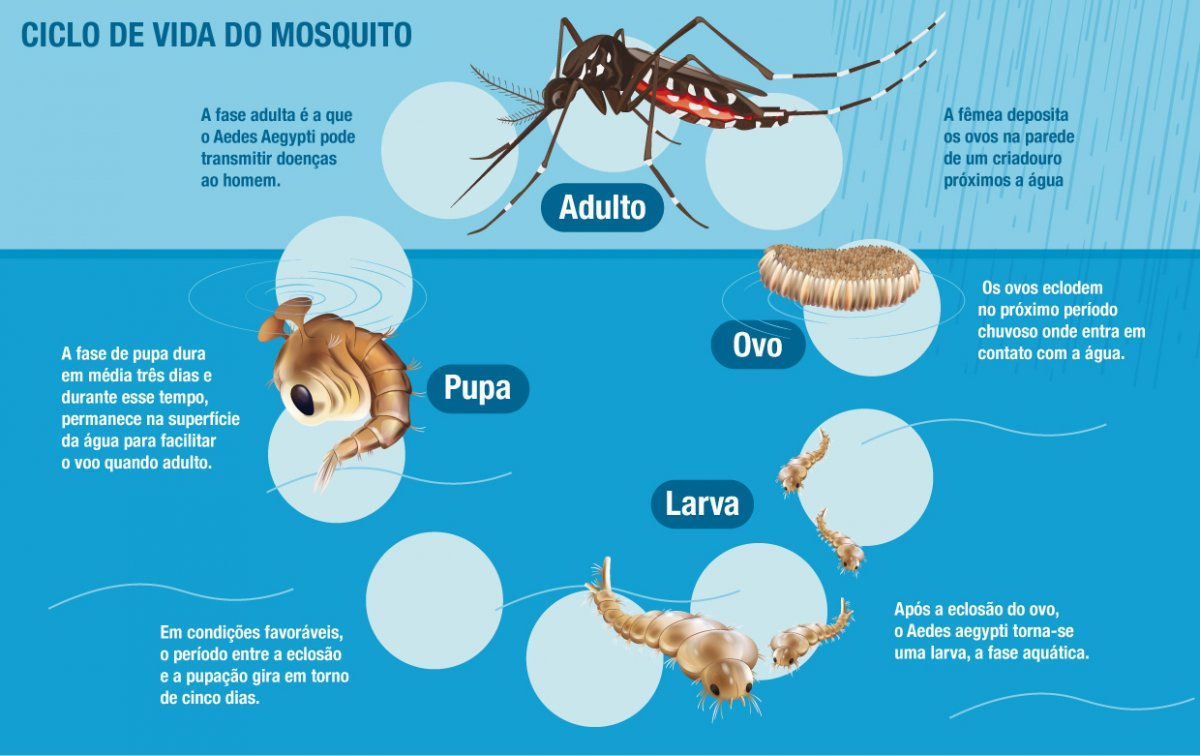
\includegraphics[width=5.90556in,height=3.72118in]{media/image37.jpeg}

PREFEITURA de Santos. Controlar mosquito ajuda a evitar três doenças -
confira infográfico. Disponível em:
\textless{}www.santos.sp.gov.br/?q=content/controlar-mosquito-ajuda-a-evitar-tres-doencas-confira-infografico\textgreater{}.
Acesso em: 19 mar. 2023.

\protect\hypertarget{_Hlk128465624}{}{}O que o infográfico está
demonstrando?

(A) As fases do mosquito \emph{Aedes aegypti}, desde o ovo até a vida
adulta.

(B) O tempo de vida do mosquito na fase adulta, que costuma durar cinco
dias.

(C) O momento que o mosquito começa a transmitir doenças, ainda como
larva.

(D) Os locais, longe de água, em que os ovos são depositados.

Saeb D4 - Identificar o tema central do texto.

BNCC EF04LP20: Reconhecer a função de gráficos, diagramas e tabelas em
textos, como forma de apresentação de dados e informações.

(A) Correta. O infográfico mostra as fases do mosquito, desde o momento
em que os ovos são depositados em criadouros próximos a água até a fase
adulta, quando já pode transmitir as doenças.

(B) Incorreta. o infográfico não cita o tempo de vida do mosquito na
fase adulta, mas o período entre a eclosão e a fase de pupa, que é de
cinco dias.

(C) Incorreta. o mosquito somente transmite doenças quando atinge a fase
adulta. (D) Incorreta. os ovos dos mosquitos são depositados próximos à
água, pois precisam estar em contato com ela no momento em que eclodem.
\end{quote}

\num{3}

\begin{quote}
Leia o infográfico a seguir.

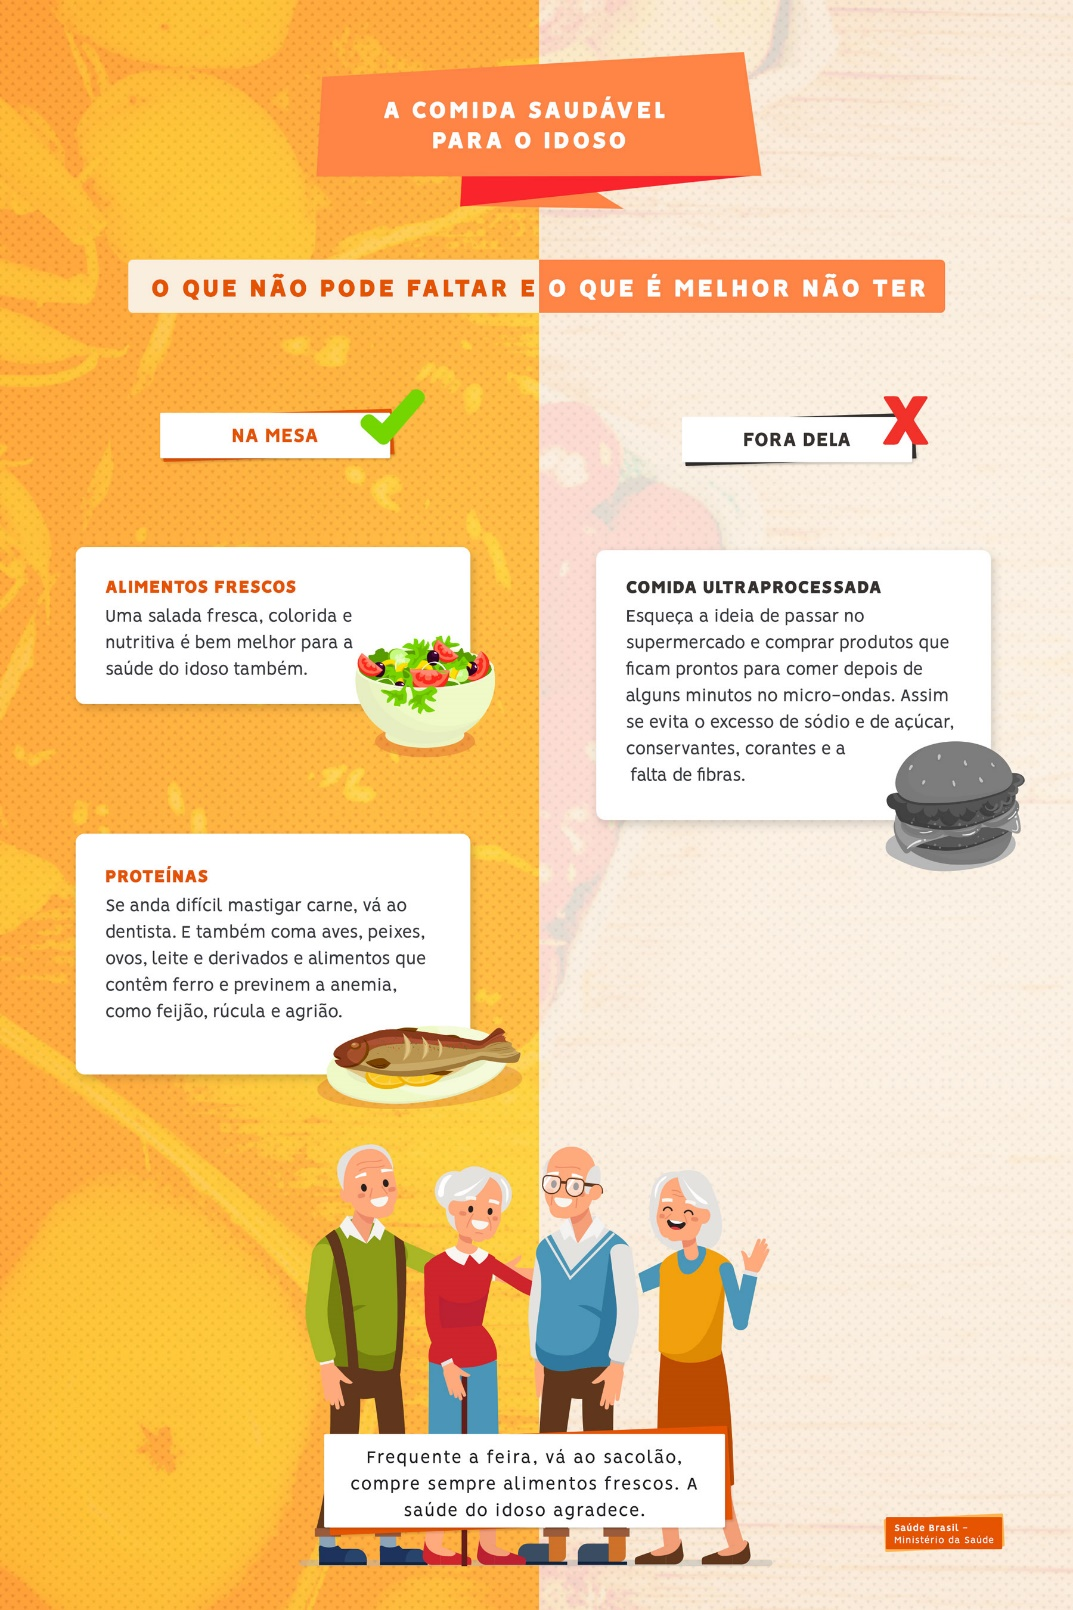
\includegraphics[width=4.87500in,height=7.31250in]{media/image38.jpeg}

CONHEÇA os fatores que influenciam a alimentação de pessoas com mais de
60 anos. Saúde Brasil, 7 nov. 2017. Disponível em:
\textless{}http://saudebrasil.saude.gov.br/eu-quero-me-alimentar-melhor/conheca-os-fatores-que-influenciam-a-alimentacao-de-pessoas-com-mais-de-60-anos\textgreater{}.
Acesso em: 19 mar. 2023.

Qual é o tema central do infográfico?

(A) As proteínas, que estão presentes em alimentos que contém muito
sódio.

(B) Os tipos de alimentos frescos que são bons para o consumo da
população.

(C) As doenças causadas pelo consumo de alimentos ultraprocessados.

(D)Os alimentos saudáveis e os não saudáveis para os idosos.

Saeb D4 - Identificar o tema central do texto.

BNCC EF35LP03 - Identificar a ideia central do texto, demonstrando
compreensão global.

(A) Incorreta. as proteínas estão presentes em alimentos saudáveis.

(B) Incorreta. o infográfico trata sobre a alimentação dos idosos, não
da população em geral.

(C) Incorreta. O infográfico não expõe as doenças causadas pelo consumo
de alimentos ultraprocessados.

(D) Correta. O infográfico mostra quais são os alimentos saudáveis e os
não saudáveis para serem consumidos por idosos.
\end{quote}

\chapter{Simulado 4}
\markboth{Simulado 4}{}

\num{1}

\begin{quote}
Leia um trecho do conto a seguir.

\textbf{O asno, o boi e o lavrador}

Um lavrador muito rico tinha várias casas no campo onde criava muitos
animais. Vivia em uma delas com a mulher e seus filhos. Ele possuía,
como Salomão, o dom de entender a língua em que falavam os animais,
embora não lhe fosse permitido traduzir o que ouvia às outras pessoas,
sob pena de perder a vida.

Tinha no mesmo curral um boi e um asno e certo dia, enquanto observava
as brincadeiras de seus filhos, ouviu o boi dizer ao asno:

- Não posso deixar de invejar tua sorte, ao ver o muito que descansas e
o pouco que trabalhas. Há um empregado que cuida de ti, te dá boa cevada
para comeres e água cristalina para beberes; e se não fossem as poucas
vezes que levas nosso dono nas curtas viagens que faz, passarias a vida
de pernas para o ar. Já a mim, tratam de modo diferente, sendo minha
situação tão desgraçada quanto é agradável a tua. Mal começa o dia, me
prendem a uma carreta, trabalho até não ter mais forças, e o lavrador,
além disso, me espanca sem parar, dando-me depois para comer algumas
favas secas. Vês que tenho razão de invejar tua sorte.

O ASNO, o boi e o lavrador. In: \emph{As mil e uma noites}: contos
árabes. Rio de Janeiro: Revan, set. 2010. 5. ed. p. 15-16.

O boi tem inveja do asno porque acha que ele

(A) entende facilmente a língua falada pelo dono deles.

(B) trabalha muito mais que ele, pois sempre acompanha o dono nas
viagens

(C) tem uma vida melhor que a dele, por não precisar trabalhar tanto.

(D) é muito mais forte do que ele por se alimentar de boa cevada.

Saeb D2 - Inferir uma afirmação implícita num texto.

BNCC EF35LP26: Ler e compreender, com certa autonomia, narrativas
ficcionais que apresentem cenários e personagens, observando os
elementos da estrutura narrativa: enredo, tempo, espaço, personagens,
narrador e a construção do discurso indireto e discurso direto.

(A) Incorreta. Quem tem o dom de entender a língua dos animais é o
lavrador, não o asno.

(B) Incorreta. O boi acredita trabalhar muito mais do que o asno.

(C) Correta. O boi inveja o asno, pois acredita que o animal não
trabalha tanto e, por isso, tem uma vida melhor que a dele.

(D) Incorreta. O boi não cita a força do asno.
\end{quote}

\num{2}

\begin{quote}
Leia o trecho do conto ``As mil e uma noites''.

{[}\ldots{}{]} Finalmente chegaram a uma região montanhosa, que era
exatamente o lugar onde o falso tio desejava por em prática o plano que
o fizera vir de um ponto extremo da África.

- Já chegamos -- disse ele a Aladin. -- E aqui poderás ver coisas
maravilhosas nunca vistas por nenhum mortal. Agora, junta algumas ervas
secas para acendermos uma fogueira.

Assim que as ervas começaram a queimar, o mágico derramou sobre elas
gotas de um perfume que trazia consigo, fazendo subir da fogueira uma
fumaça espessa, enquanto pronunciava palavras estranhas que Aladin não
compreendia. Nesse momento, a terra estremeceu e se abriu diante dos
dois, deixando ver uma pedra quadrada de mais ou menos 60 centímetros de
lado e 30 centímetros de espessura, tendo ao centro uma argola de metal
que servia para levantá-la. Aladin, assustado com o que acontecia,
tentou fugir, mas foi detido pelo mágico, que o atingiu com um soco no
rosto, tão forte que o derrubou. Aladin, chorando, falou:

- Tio, que fiz eu para me baterdes deste modo?

- Tenho minhas razões. Sou teu tio e faço as vezes de teu pai, de modo
que tens de me obedecer. Mas, meu caro sobrinho, se fizerdes exatamente
o que eu mando serás muito bem recompensado.

Essas palavras aliviara um pouco o temor e o ressentimento de Aladin.

\protect\hypertarget{_Hlk36965909}{}{}A HISTÓRIA de Aladin e a lâmpada
maravilhosa\emph{.} In: \emph{As mil e uma noites}: contos árabes. Rio
de Janeiro: Revan, set. 2010. 5. ed. p. 144.

De acordo com o trecho, o mágico está

(A) mostrando-se assustado com as palavras inteligíveis pronunciadas
pelo sobrinho.

(B) apresentando a Aladin uma região montanhosa, situada em um ponto da
África.

(C) ajudando o sobrinho Aladin, ensinando-o a fazer magias na parte
extrema da África.

(D) fingindo ser o tio de Aladin, apenas para o atrair e poder dar
início aos seus planos.

Saeb D3 - Estabelecer relação entre informações num texto ou entre
diferentes textos.

BNCC EF35LP26: Ler e compreender, com certa autonomia, narrativas
ficcionais que apresentem cenários e personagens, observando os
elementos da estrutura narrativa: enredo, tempo, espaço, personagens,
narrador e a construção do discurso indireto e discurso direto.

(A) Incorreta. Quem se mostra assustado é Aladin, e não o mágico.

(B) Incorreta. O mágico tem a intenção de levar Aladin para a esse local
e colocar em prática seus planos.

(C) Incorreta. O mágico não ensina magias ao Aladin.

(D) Correta. O mágico é, na realidade, um falso tio.
\end{quote}

\num{3}

\begin{quote}
Leia, a seguir, o trecho de uma notícia que aborda o Dia do
Cooperativismo.

\textbf{Dia do Cooperativismo é celebrado em várias cidades brasileiras}

{[}...{]} ``O cooperativismo trabalha na linha de frente do
desenvolvimento socioeconômico do país. E o Dia de Cooperar é uma forma
de expressar a força do nosso movimento, que por meio de ações
voluntárias, ajuda pessoas a transformarem suas vidas'', afirma o
presidente do Sindicato e Organização das Cooperativas do Estado do Rio
(OCB/RJ), Vinícius Mesquita.

ABDALA, Vitor. Dia do Cooperativismo é celebrado em várias cidades
brasileiras. Agência Brasil. Disponível em:
http://agenciabrasil.ebc.com.br/economia/noticia/2019-07/dia-do-

cooperativismo-e-celebrado-em-varias-cidades-brasileiras. Acesso em: 19
mar. 2023.

No trecho, o autor insere a declaração de uma pessoa com a intenção de

(A) dar credibilidade à notícia.

(B) dar destaque a aspectos importantes.

(C) fazer um complemento ao título.

(D) ilustrar o que foi relatado.

Saeb D3 - Estabelecer relação entre informações num texto ou entre
diferentes textos.

BNCC EF35LP16 - Identificar e reproduzir, em notícias, manchetes, lides
e corpo de notícias simples para público infantil e cartas de reclamação
(revista infantil), digitais ou impressos, a formatação e diagramação
específica de cada um desses gêneros, inclusive em suas versões orais.

(A) Correta. O autor insere a declaração de uma pessoa com a intenção de
dar credibilidade à notícia.

(B) Incorreta. O título tem a função de destacar os aspectos mais
importantes do fato relatado.

(C) Incorreta. A linha fina complementa as informações apresentadas no
título.

(D) Incorreta. Não há imagens ilustrando os fatos.
\end{quote}

\num{4}

\begin{quote}
Leia o trecho retirado de uma entrevista com um aluno de 7 anos de idade
sobre futebol do jornal Folha de S. Paulo.

Estudante da escola pública estadual Professor Laerte Panighel,
{[}...{]} o garoto de 7 anos se revelou {[}...{]} esperto desde a
primeira visita da reportagem ao colégio. {[}...{]}

\textbf{Por que tem muito corintiano nessa escola?}

Porque o Corinthians tá ganhando de todos os times. O Palmeiras perdeu
de 1 x 0. Então aqui o Corinthians é mais participado, {[}...{]} se o
Palmeiras ganhar vai ser todo mundo ser palmeirense.

\textbf{Ah, o time depende de se está ganhando ou não...}

É. É todo mundo assim. Menos eu. Eu sou só corintiano. Nem que perca,
nem

que ganhe.

VICTOR, Fábio. ``Não importa para que time você torce, o que importa é a
amizade'', diz Ryan, 7. Folha de S. Paulo. Disponível em:
\&lt;http://temas.folha.uol.com.br/crianca-do-dia/esporte/nao-importa-pra-que-time-voce-torce-o-que-importa-e-a-amizade-diz-ryan-7.shtml\&gt;.
Acesso em: 19

mar. 2023.

Conforme informações do texto, o aluno

(A) muda de time a cada partida, torcendo sempre para o vencedor.

(B) torce para o mesmo time que a maioria da escola, o Palmeiras.

(C) não entende por que seus colegas mudam de time o tempo todo.

(D) gosta muito do mesmo time e não muda sua torcida por nada.

Saeb D1 - Localizar informações num texto.

BNCC EF15LP03: Localizar informações explícitas em textos.

(A) Incorreta. O aluno é o único da escola que não muda de time

(B) Incorreta. Esse time é o Corinthians e não o Palmeiras.

(C) Incorreta. Ele entende o motivo de os seus amigos trocarem de time.

(D) Correta. O entrevistado, tem um único time, do qual gosta muito e
não muda sua opinião.
\end{quote}

\chapter{Referências}
\markboth{Referências}{}

\begin{quote}
BRASIL. Ministério da Educação. \textbf{Base nacional comum curricular}:
educação é a base.

BRASIL. Ministério da Educação. \textbf{Pacto nacional pela
alfabetização na idade certa}. Disponível em:
\textless{}http://www.serdigital.com.br/gerenciador/clientes/ceel/material/149.pdf\textgreater{}.
Acesso em: fev. 2023.

KAUFMAN, Ana María; RODRÍGUEZ, María Helena. \textbf{Escola, leitura e
produção de textos}. Porto Alegre: Artmed, 1995.

KOCH, Ingedore G. Villaça. \textbf{Ler e escrever}: estratégias de
produção textual. São Paulo: Contexto, 2010.

LERNER, Delia. \textbf{Ler e escrever na escola}: o real, o possível e o
necessário. Porto Alegre: Artmed, 2002.

NÓBREGA, Maria José. \textbf{Ortografia}. São Paulo: Melhoramentos,
2013.
\end{quote}

\chapter{Sites}
\markboth{Sites}{}

\begin{quote}
\textbf{Ciência Hoje das Crianças}. Disponível em:
\textless{}http://chc.org.br/\textgreater{}. Acesso em: fev. 2023.

\textbf{DOMÍNIO PÙBLICO}. Disponível em:
\url{http://www.dominiopublico.gov.br/pesquisa/PesquisaObraForm.jsp}.
Acesso em: 28 fev. 2023.

\textbf{RÁDIOS EBC}. Disponível em: https://radios.ebc.com.br/. Acesso
em: 23 fev. 2023.

\textbf{PORTAL Teatro na escola}. Disponível em:
\url{https://www.teatronaescola.com/}. Acesso em: 28 fev. 2023.
\end{quote}
